\documentclass[twoside]{book}

% Packages required by doxygen
\usepackage{fixltx2e}
\usepackage{calc}
\usepackage{doxygen}
\usepackage[export]{adjustbox} % also loads graphicx
\usepackage{graphicx}
\usepackage[utf8]{inputenc}
\usepackage{makeidx}
\usepackage{multicol}
\usepackage{multirow}
\PassOptionsToPackage{warn}{textcomp}
\usepackage{textcomp}
\usepackage[nointegrals]{wasysym}
\usepackage[table]{xcolor}

% Font selection
\usepackage[T1]{fontenc}
\usepackage[scaled=.90]{helvet}
\usepackage{courier}
\usepackage{amssymb}
\usepackage{sectsty}
\renewcommand{\familydefault}{\sfdefault}
\allsectionsfont{%
  \fontseries{bc}\selectfont%
  \color{darkgray}%
}
\renewcommand{\DoxyLabelFont}{%
  \fontseries{bc}\selectfont%
  \color{darkgray}%
}
\newcommand{\+}{\discretionary{\mbox{\scriptsize$\hookleftarrow$}}{}{}}

% Page & text layout
\usepackage{geometry}
\geometry{%
  a4paper,%
  top=2.5cm,%
  bottom=2.5cm,%
  left=2.5cm,%
  right=2.5cm%
}
\tolerance=750
\hfuzz=15pt
\hbadness=750
\setlength{\emergencystretch}{15pt}
\setlength{\parindent}{0cm}
\setlength{\parskip}{3ex plus 2ex minus 2ex}
\makeatletter
\renewcommand{\paragraph}{%
  \@startsection{paragraph}{4}{0ex}{-1.0ex}{1.0ex}{%
    \normalfont\normalsize\bfseries\SS@parafont%
  }%
}
\renewcommand{\subparagraph}{%
  \@startsection{subparagraph}{5}{0ex}{-1.0ex}{1.0ex}{%
    \normalfont\normalsize\bfseries\SS@subparafont%
  }%
}
\makeatother

% Headers & footers
\usepackage{fancyhdr}
\pagestyle{fancyplain}
\fancyhead[LE]{\fancyplain{}{\bfseries\thepage}}
\fancyhead[CE]{\fancyplain{}{}}
\fancyhead[RE]{\fancyplain{}{\bfseries\leftmark}}
\fancyhead[LO]{\fancyplain{}{\bfseries\rightmark}}
\fancyhead[CO]{\fancyplain{}{}}
\fancyhead[RO]{\fancyplain{}{\bfseries\thepage}}
\fancyfoot[LE]{\fancyplain{}{}}
\fancyfoot[CE]{\fancyplain{}{}}
\fancyfoot[RE]{\fancyplain{}{\bfseries\scriptsize Generated by Doxygen }}
\fancyfoot[LO]{\fancyplain{}{\bfseries\scriptsize Generated by Doxygen }}
\fancyfoot[CO]{\fancyplain{}{}}
\fancyfoot[RO]{\fancyplain{}{}}
\renewcommand{\footrulewidth}{0.4pt}
\renewcommand{\chaptermark}[1]{%
  \markboth{#1}{}%
}
\renewcommand{\sectionmark}[1]{%
  \markright{\thesection\ #1}%
}

% Indices & bibliography
\usepackage{natbib}
\usepackage[titles]{tocloft}
\setcounter{tocdepth}{3}
\setcounter{secnumdepth}{5}
\makeindex

% Hyperlinks (required, but should be loaded last)
\usepackage{ifpdf}
\ifpdf
  \usepackage[pdftex,pagebackref=true]{hyperref}
\else
  \usepackage[ps2pdf,pagebackref=true]{hyperref}
\fi
\hypersetup{%
  colorlinks=true,%
  linkcolor=blue,%
  citecolor=blue,%
  unicode%
}

% Custom commands
\newcommand{\clearemptydoublepage}{%
  \newpage{\pagestyle{empty}\cleardoublepage}%
}

\usepackage{caption}
\captionsetup{labelsep=space,justification=centering,font={bf},singlelinecheck=off,skip=4pt,position=top}

%===== C O N T E N T S =====

\begin{document}

% Titlepage & ToC
\hypersetup{pageanchor=false,
             bookmarksnumbered=true,
             pdfencoding=unicode
            }
\pagenumbering{alph}
\begin{titlepage}
\vspace*{7cm}
\begin{center}%
{\Large AtoD }\\
\vspace*{1cm}
{\large Generated by Doxygen 1.8.12}\\
\end{center}
\end{titlepage}
\clearemptydoublepage
\pagenumbering{roman}
\tableofcontents
\clearemptydoublepage
\pagenumbering{arabic}
\hypersetup{pageanchor=true}

%--- Begin generated contents ---
\chapter{Data description}
\label{md_atod_data__r_e_a_d_m_e}
\hypertarget{md_atod_data__r_e_a_d_m_e}{}
All the data used by app is stored in Ato\+D.\+db. All $\ast$.json files are temporary.

\subsection*{abilities\+\_\+changes.\+json}

This file defines changes in abilities descriptions.

There are similar properties which could be merged to one property, this file defines mapping from old names to the new ones.

{\bfseries I\+M\+P\+O\+R\+T\+A\+NT\+:} mappings there value equal to one of the capitalized properties\+: Ability\+Damage, Ability\+Cooldown... should be defined at the {\itshape end of file}, after everything. 
\chapter{Namespace Index}
\section{Namespace List}
Here is a list of all documented namespaces with brief descriptions\+:\begin{DoxyCompactList}
\item\contentsline{section}{\hyperlink{namespaceatod_1_1abilities}{atod.\+abilities} }{\pageref{namespaceatod_1_1abilities}}{}
\item\contentsline{section}{\hyperlink{namespaceatod_1_1db_1_1schemas}{atod.\+db.\+schemas} }{\pageref{namespaceatod_1_1db_1_1schemas}}{}
\item\contentsline{section}{\hyperlink{namespaceatod_1_1db_1_1setup}{atod.\+db.\+setup} }{\pageref{namespaceatod_1_1db_1_1setup}}{}
\item\contentsline{section}{\hyperlink{namespaceatod_1_1discovery}{atod.\+discovery} }{\pageref{namespaceatod_1_1discovery}}{}
\item\contentsline{section}{\hyperlink{namespaceatod_1_1files}{atod.\+files} }{\pageref{namespaceatod_1_1files}}{}
\item\contentsline{section}{\hyperlink{namespaceatod_1_1interfaces}{atod.\+interfaces} }{\pageref{namespaceatod_1_1interfaces}}{}
\item\contentsline{section}{\hyperlink{namespaceatod_1_1ml_1_1abilities}{atod.\+ml.\+abilities} }{\pageref{namespaceatod_1_1ml_1_1abilities}}{}
\item\contentsline{section}{\hyperlink{namespaceatod_1_1preprocessing_1_1abilities}{atod.\+preprocessing.\+abilities} }{\pageref{namespaceatod_1_1preprocessing_1_1abilities}}{}
\item\contentsline{section}{\hyperlink{namespaceatod_1_1preprocessing_1_1dictionary}{atod.\+preprocessing.\+dictionary} }{\pageref{namespaceatod_1_1preprocessing_1_1dictionary}}{}
\item\contentsline{section}{\hyperlink{namespaceatod_1_1preprocessing_1_1json2rows}{atod.\+preprocessing.\+json2rows} }{\pageref{namespaceatod_1_1preprocessing_1_1json2rows}}{}
\item\contentsline{section}{\hyperlink{namespaceatod_1_1preprocessing_1_1txt2json}{atod.\+preprocessing.\+txt2json} }{\pageref{namespaceatod_1_1preprocessing_1_1txt2json}}{}
\end{DoxyCompactList}

\chapter{Hierarchical Index}
\section{Class Hierarchy}
This inheritance list is sorted roughly, but not completely, alphabetically\+:\begin{DoxyCompactList}
\item \contentsline{section}{atod.\+interfaces.\+Group}{\pageref{classatod_1_1interfaces_1_1_group}}{}
\begin{DoxyCompactList}
\item \contentsline{section}{atod.\+abilities.\+Abilities}{\pageref{classatod_1_1abilities_1_1_abilities}}{}
\item \contentsline{section}{atod.\+heroes.\+Heroes}{\pageref{classatod_1_1heroes_1_1_heroes}}{}
\end{DoxyCompactList}
\item \contentsline{section}{atod.\+interfaces.\+Member}{\pageref{classatod_1_1interfaces_1_1_member}}{}
\begin{DoxyCompactList}
\item \contentsline{section}{atod.\+abilities.\+Ability}{\pageref{classatod_1_1abilities_1_1_ability}}{}
\item \contentsline{section}{atod.\+heroes.\+Hero}{\pageref{classatod_1_1heroes_1_1_hero}}{}
\end{DoxyCompactList}
\item Test\+Case\begin{DoxyCompactList}
\item \contentsline{section}{atod.\+tests.\+test\+\_\+cleaninng\+\_\+abilities.\+Test\+Cleaning\+Abilities}{\pageref{classatod_1_1tests_1_1test__cleaninng__abilities_1_1_test_cleaning_abilities}}{}
\item \contentsline{section}{atod.\+tests.\+test\+\_\+dictionary.\+Test\+Dictionary}{\pageref{classatod_1_1tests_1_1test__dictionary_1_1_test_dictionary}}{}
\item \contentsline{section}{atod.\+tests.\+test\+\_\+hero.\+Test\+Hero}{\pageref{classatod_1_1tests_1_1test__hero_1_1_test_hero}}{}
\item \contentsline{section}{atod.\+tests.\+test\+\_\+hero\+\_\+model.\+My\+Test\+Case}{\pageref{classatod_1_1tests_1_1test__hero__model_1_1_my_test_case}}{}
\item \contentsline{section}{atod.\+tests.\+test\+\_\+json2vectors.\+Test\+Json2\+Vectors}{\pageref{classatod_1_1tests_1_1test__json2vectors_1_1_test_json2_vectors}}{}
\item \contentsline{section}{atod.\+tests.\+test\+\_\+settings.\+Test\+Settings}{\pageref{classatod_1_1tests_1_1test__settings_1_1_test_settings}}{}
\item \contentsline{section}{atod.\+tests.\+test\+\_\+to\+\_\+json.\+Test\+Parser}{\pageref{classatod_1_1tests_1_1test__to__json_1_1_test_parser}}{}
\item \contentsline{section}{atod.\+tests.\+test\+\_\+to\+\_\+rows.\+Test\+Utils\+DB}{\pageref{classatod_1_1tests_1_1test__to__rows_1_1_test_utils_d_b}}{}
\end{DoxyCompactList}
\item Base\begin{DoxyCompactList}
\item \contentsline{section}{atod.\+models.\+ability.\+Ability\+Model}{\pageref{classatod_1_1models_1_1ability_1_1_ability_model}}{}
\item \contentsline{section}{atod.\+models.\+hero.\+Hero\+Model}{\pageref{classatod_1_1models_1_1hero_1_1_hero_model}}{}
\item \contentsline{section}{atod.\+models.\+item.\+Item\+Model}{\pageref{classatod_1_1models_1_1item_1_1_item_model}}{}
\end{DoxyCompactList}
\item Base\begin{DoxyCompactList}
\item \contentsline{section}{atod.\+models.\+ability\+\_\+specs.\+Ability\+Specs\+Model}{\pageref{classatod_1_1models_1_1ability__specs_1_1_ability_specs_model}}{}
\item \contentsline{section}{atod.\+models.\+ability\+\_\+texts.\+Ability\+Texts\+Model}{\pageref{classatod_1_1models_1_1ability__texts_1_1_ability_texts_model}}{}
\end{DoxyCompactList}
\end{DoxyCompactList}

\chapter{Class Index}
\section{Class List}
Here are the classes, structs, unions and interfaces with brief descriptions\+:\begin{DoxyCompactList}
\item\contentsline{section}{\hyperlink{classatod_1_1abilities_1_1_abilities}{atod.\+abilities.\+Abilities} }{\pageref{classatod_1_1abilities_1_1_abilities}}{}
\item\contentsline{section}{\hyperlink{classabilities__old_1_1_abilities}{abilities\+\_\+old.\+Abilities} }{\pageref{classabilities__old_1_1_abilities}}{}
\item\contentsline{section}{\hyperlink{classatod_1_1abilities_1_1_ability}{atod.\+abilities.\+Ability} }{\pageref{classatod_1_1abilities_1_1_ability}}{}
\item\contentsline{section}{\hyperlink{classatod_1_1models_1_1ability_1_1_ability_model}{atod.\+models.\+ability.\+Ability\+Model} }{\pageref{classatod_1_1models_1_1ability_1_1_ability_model}}{}
\item\contentsline{section}{\hyperlink{classatod_1_1models_1_1ability__specs_1_1_ability_specs_model}{atod.\+models.\+ability\+\_\+specs.\+Ability\+Specs\+Model} }{\pageref{classatod_1_1models_1_1ability__specs_1_1_ability_specs_model}}{}
\item\contentsline{section}{\hyperlink{classatod_1_1models_1_1ability__texts_1_1_ability_texts_model}{atod.\+models.\+ability\+\_\+texts.\+Ability\+Texts\+Model} }{\pageref{classatod_1_1models_1_1ability__texts_1_1_ability_texts_model}}{}
\item\contentsline{section}{\hyperlink{classatod_1_1interfaces_1_1_group}{atod.\+interfaces.\+Group} }{\pageref{classatod_1_1interfaces_1_1_group}}{}
\item\contentsline{section}{\hyperlink{classhero_1_1_hero}{hero.\+Hero} }{\pageref{classhero_1_1_hero}}{}
\item\contentsline{section}{\hyperlink{classatod_1_1heroes_1_1_hero}{atod.\+heroes.\+Hero} }{\pageref{classatod_1_1heroes_1_1_hero}}{}
\item\contentsline{section}{\hyperlink{classatod_1_1heroes_1_1_heroes}{atod.\+heroes.\+Heroes} }{\pageref{classatod_1_1heroes_1_1_heroes}}{}
\item\contentsline{section}{\hyperlink{classatod_1_1models_1_1hero_1_1_hero_model}{atod.\+models.\+hero.\+Hero\+Model} }{\pageref{classatod_1_1models_1_1hero_1_1_hero_model}}{}
\item\contentsline{section}{\hyperlink{classatod_1_1models_1_1item_1_1_item_model}{atod.\+models.\+item.\+Item\+Model} }{\pageref{classatod_1_1models_1_1item_1_1_item_model}}{}
\item\contentsline{section}{\hyperlink{classleague_1_1_league}{league.\+League} }{\pageref{classleague_1_1_league}}{}
\item\contentsline{section}{\hyperlink{classmatch_1_1_match}{match.\+Match} }{\pageref{classmatch_1_1_match}}{}
\item\contentsline{section}{\hyperlink{classatod_1_1interfaces_1_1_member}{atod.\+interfaces.\+Member} }{\pageref{classatod_1_1interfaces_1_1_member}}{}
\item\contentsline{section}{\hyperlink{classatod_1_1tests_1_1test__hero__model_1_1_my_test_case}{atod.\+tests.\+test\+\_\+hero\+\_\+model.\+My\+Test\+Case} }{\pageref{classatod_1_1tests_1_1test__hero__model_1_1_my_test_case}}{}
\item\contentsline{section}{\hyperlink{classpick_1_1_pick}{pick.\+Pick} }{\pageref{classpick_1_1_pick}}{}
\item\contentsline{section}{\hyperlink{classplayer_1_1_player}{player.\+Player} }{\pageref{classplayer_1_1_player}}{}
\item\contentsline{section}{\hyperlink{classabilities__old_1_1_singleton}{abilities\+\_\+old.\+Singleton} }{\pageref{classabilities__old_1_1_singleton}}{}
\item\contentsline{section}{\hyperlink{classteam_1_1_team}{team.\+Team} }{\pageref{classteam_1_1_team}}{}
\item\contentsline{section}{\hyperlink{classtest__abilities_1_1_test_abilities}{test\+\_\+abilities.\+Test\+Abilities} }{\pageref{classtest__abilities_1_1_test_abilities}}{}
\item\contentsline{section}{\hyperlink{classatod_1_1tests_1_1test__cleaninng__abilities_1_1_test_cleaning_abilities}{atod.\+tests.\+test\+\_\+cleaninng\+\_\+abilities.\+Test\+Cleaning\+Abilities} }{\pageref{classatod_1_1tests_1_1test__cleaninng__abilities_1_1_test_cleaning_abilities}}{}
\item\contentsline{section}{\hyperlink{classatod_1_1tests_1_1test__dictionary_1_1_test_dictionary}{atod.\+tests.\+test\+\_\+dictionary.\+Test\+Dictionary} }{\pageref{classatod_1_1tests_1_1test__dictionary_1_1_test_dictionary}}{}
\item\contentsline{section}{\hyperlink{classatod_1_1tests_1_1test__hero_1_1_test_hero}{atod.\+tests.\+test\+\_\+hero.\+Test\+Hero} }{\pageref{classatod_1_1tests_1_1test__hero_1_1_test_hero}}{}
\item\contentsline{section}{\hyperlink{classatod_1_1tests_1_1test__json2vectors_1_1_test_json2_vectors}{atod.\+tests.\+test\+\_\+json2vectors.\+Test\+Json2\+Vectors} }{\pageref{classatod_1_1tests_1_1test__json2vectors_1_1_test_json2_vectors}}{}
\item\contentsline{section}{\hyperlink{classatod_1_1tests_1_1test__to__json_1_1_test_parser}{atod.\+tests.\+test\+\_\+to\+\_\+json.\+Test\+Parser} }{\pageref{classatod_1_1tests_1_1test__to__json_1_1_test_parser}}{}
\item\contentsline{section}{\hyperlink{classatod_1_1tests_1_1test__settings_1_1_test_settings}{atod.\+tests.\+test\+\_\+settings.\+Test\+Settings} }{\pageref{classatod_1_1tests_1_1test__settings_1_1_test_settings}}{}
\item\contentsline{section}{\hyperlink{classtest__abilities_1_1_test_tools_abilities}{test\+\_\+abilities.\+Test\+Tools\+Abilities} }{\pageref{classtest__abilities_1_1_test_tools_abilities}}{}
\item\contentsline{section}{\hyperlink{classatod_1_1tests_1_1test__to__rows_1_1_test_utils_d_b}{atod.\+tests.\+test\+\_\+to\+\_\+rows.\+Test\+Utils\+DB} }{\pageref{classatod_1_1tests_1_1test__to__rows_1_1_test_utils_d_b}}{}
\end{DoxyCompactList}

\chapter{Namespace Documentation}
\hypertarget{namespaceatod_1_1abilities}{}\section{atod.\+abilities Namespace Reference}
\label{namespaceatod_1_1abilities}\index{atod.\+abilities@{atod.\+abilities}}
\subsection*{Classes}
\begin{DoxyCompactItemize}
\item 
class \hyperlink{classatod_1_1abilities_1_1_abilities}{Abilities}
\item 
class \hyperlink{classatod_1_1abilities_1_1_ability}{Ability}
\end{DoxyCompactItemize}


\subsection{Detailed Description}
\begin{DoxyVerb}This module describes single hero ability.\end{DoxyVerb}
 
\hypertarget{namespaceatod_1_1db_1_1schemas}{}\section{atod.\+db.\+schemas Namespace Reference}
\label{namespaceatod_1_1db_1_1schemas}\index{atod.\+db.\+schemas@{atod.\+db.\+schemas}}
\subsection*{Variables}
\begin{DoxyCompactItemize}
\item 
{\bfseries level}\hypertarget{namespaceatod_1_1db_1_1schemas_a4a7ea01e71903882d0dd27d6090d429c}{}\label{namespaceatod_1_1db_1_1schemas_a4a7ea01e71903882d0dd27d6090d429c}

\item 
dictionary {\bfseries field\+\_\+format}
\item 
dictionary {\bfseries type\+\_\+to\+\_\+string}
\item 
list {\bfseries L\+A\+B\+E\+LS}
\end{DoxyCompactItemize}


\subsection{Detailed Description}
\begin{DoxyVerb}There are a lot of variables in descriptions of every subject in the
game, so db schemas are pretty complex to write in static form.
This file provides interface to all schemas through function calls.
\end{DoxyVerb}
 

\subsection{Variable Documentation}
\index{atod\+::db\+::schemas@{atod\+::db\+::schemas}!field\+\_\+format@{field\+\_\+format}}
\index{field\+\_\+format@{field\+\_\+format}!atod\+::db\+::schemas@{atod\+::db\+::schemas}}
\subsubsection[{\texorpdfstring{field\+\_\+format}{field\_format}}]{\setlength{\rightskip}{0pt plus 5cm}dictionary atod.\+db.\+schemas.\+field\+\_\+format}\hypertarget{namespaceatod_1_1db_1_1schemas_a7f12079a3333d78633ae8abf845e7627}{}\label{namespaceatod_1_1db_1_1schemas_a7f12079a3333d78633ae8abf845e7627}
{\bfseries Initial value\+:}
\begin{DoxyCode}
1 = \{
2     \textcolor{stringliteral}{'FIELD\_FLOAT'}: Float,
3     \textcolor{stringliteral}{'FIELD\_INTEGER'}: Integer,
4     \textcolor{stringliteral}{'FIELD\_STRING'}: String,
5     int: Integer,
6     str: String,
7     float: Float
8 \}
\end{DoxyCode}
\index{atod\+::db\+::schemas@{atod\+::db\+::schemas}!L\+A\+B\+E\+LS@{L\+A\+B\+E\+LS}}
\index{L\+A\+B\+E\+LS@{L\+A\+B\+E\+LS}!atod\+::db\+::schemas@{atod\+::db\+::schemas}}
\subsubsection[{\texorpdfstring{L\+A\+B\+E\+LS}{LABELS}}]{\setlength{\rightskip}{0pt plus 5cm}list atod.\+db.\+schemas.\+L\+A\+B\+E\+LS}\hypertarget{namespaceatod_1_1db_1_1schemas_a903269021db6731cb07d184db3547126}{}\label{namespaceatod_1_1db_1_1schemas_a903269021db6731cb07d184db3547126}
{\bfseries Initial value\+:}
\begin{DoxyCode}
1 = [\textcolor{stringliteral}{'stun'}, \textcolor{stringliteral}{'transformation'}, \textcolor{stringliteral}{'slow'}, \textcolor{stringliteral}{'durability'}, \textcolor{stringliteral}{'nuke'},
2           \textcolor{stringliteral}{'escape'}, \textcolor{stringliteral}{'non\_hero'}, \textcolor{stringliteral}{'attack\_bonus'}, \textcolor{stringliteral}{'heal'},
3           \textcolor{stringliteral}{'based\_on\_attr'}, \textcolor{stringliteral}{'aoe'}, \textcolor{stringliteral}{'period\_damage'}, \textcolor{stringliteral}{'attack\_debuff'},
4           \textcolor{stringliteral}{'invis'}, \textcolor{stringliteral}{'vision'}, \textcolor{stringliteral}{'silence'}, \textcolor{stringliteral}{'lifesteal'}, \textcolor{stringliteral}{'armor\_buff'},
5           \textcolor{stringliteral}{'armor\_debuff'}, \textcolor{stringliteral}{'save'}, \textcolor{stringliteral}{'move\_speed\_buff'}, \textcolor{stringliteral}{'illusions'}, \textcolor{stringliteral}{'chance'},
6           \textcolor{stringliteral}{'multiply\_heroes'}, \textcolor{stringliteral}{'global'}, \textcolor{stringliteral}{'shield'}, \textcolor{stringliteral}{'attribute\_gain'},
7           \textcolor{stringliteral}{'amplify\_magic\_dmg'}, \textcolor{stringliteral}{'summon\_unit'}, \textcolor{stringliteral}{'regen'}, \textcolor{stringliteral}{'daytime\_dependent'},
8           \textcolor{stringliteral}{'stacks'}, \textcolor{stringliteral}{'purge'}, \textcolor{stringliteral}{'in\_percents'}]
\end{DoxyCode}
\index{atod\+::db\+::schemas@{atod\+::db\+::schemas}!type\+\_\+to\+\_\+string@{type\+\_\+to\+\_\+string}}
\index{type\+\_\+to\+\_\+string@{type\+\_\+to\+\_\+string}!atod\+::db\+::schemas@{atod\+::db\+::schemas}}
\subsubsection[{\texorpdfstring{type\+\_\+to\+\_\+string}{type\_to\_string}}]{\setlength{\rightskip}{0pt plus 5cm}dictionary atod.\+db.\+schemas.\+type\+\_\+to\+\_\+string}\hypertarget{namespaceatod_1_1db_1_1schemas_aefa901273797ca2b811b16aa70d5d6db}{}\label{namespaceatod_1_1db_1_1schemas_aefa901273797ca2b811b16aa70d5d6db}
{\bfseries Initial value\+:}
\begin{DoxyCode}
1 = \{
2     int: \textcolor{stringliteral}{'FIELD\_INTEGER'},
3     str: \textcolor{stringliteral}{'FIELD\_STRING'},
4     float: \textcolor{stringliteral}{'FIELD\_FLOAT'},
5     Float: \textcolor{stringliteral}{'FIELD\_FLOAT'},
6     Integer: \textcolor{stringliteral}{'FIELD\_INTEGER'},
7     String: \textcolor{stringliteral}{'FIELD\_STRING'},
8 \}
\end{DoxyCode}

\hypertarget{namespaceatod_1_1db_1_1setup}{}\section{atod.\+db.\+setup Namespace Reference}
\label{namespaceatod_1_1db_1_1setup}\index{atod.\+db.\+setup@{atod.\+db.\+setup}}
\subsection*{Variables}
\begin{DoxyCompactItemize}
\item 
{\bfseries engine} = create\+\_\+engine(\textquotesingle{}sqlite\+:///\textquotesingle{} + settings.\+D\+B\+\_\+\+P\+A\+TH)\hypertarget{namespaceatod_1_1db_1_1setup_a5339d3ba73c5603c6683ef6097ff2f75}{}\label{namespaceatod_1_1db_1_1setup_a5339d3ba73c5603c6683ef6097ff2f75}

\item 
{\bfseries Base} = declarative\+\_\+base()\hypertarget{namespaceatod_1_1db_1_1setup_a16d34167d9d279b13228df8d9a54616b}{}\label{namespaceatod_1_1db_1_1setup_a16d34167d9d279b13228df8d9a54616b}

\item 
{\bfseries Session} = sessionmaker(bind=engine)\hypertarget{namespaceatod_1_1db_1_1setup_a5d0e717678c8672f26543f30d5c3863b}{}\label{namespaceatod_1_1db_1_1setup_a5d0e717678c8672f26543f30d5c3863b}

\item 
{\bfseries session} = Session()\hypertarget{namespaceatod_1_1db_1_1setup_ad6cd914bec0c956246066261db62ef28}{}\label{namespaceatod_1_1db_1_1setup_ad6cd914bec0c956246066261db62ef28}

\end{DoxyCompactItemize}


\subsection{Detailed Description}
\begin{DoxyVerb}Setting up database. \end{DoxyVerb}
 
\hypertarget{namespaceatod_1_1discovery}{}\section{atod.\+discovery Namespace Reference}
\label{namespaceatod_1_1discovery}\index{atod.\+discovery@{atod.\+discovery}}
\subsection*{Functions}
\begin{DoxyCompactItemize}
\item 
def {\bfseries check} ()\hypertarget{namespaceatod_1_1discovery_a30d07b0bced84b223e86785e4d3d9886}{}\label{namespaceatod_1_1discovery_a30d07b0bced84b223e86785e4d3d9886}

\item 
def {\bfseries get\+\_\+all\+\_\+types} ()\hypertarget{namespaceatod_1_1discovery_ae6f4fa5a923111a3775dfb0f52f20719}{}\label{namespaceatod_1_1discovery_ae6f4fa5a923111a3775dfb0f52f20719}

\end{DoxyCompactItemize}


\subsection{Detailed Description}
\begin{DoxyVerb}Set of functions which help to understand data and see what can be
cleaned.
In future this file would provide functions to take a look at the overall
data, for example amount of abilities, heroes...
\end{DoxyVerb}
 
\hypertarget{namespaceatod_1_1files}{}\section{atod.\+files Namespace Reference}
\label{namespaceatod_1_1files}\index{atod.\+files@{atod.\+files}}
\subsection*{Functions}
\begin{DoxyCompactItemize}
\item 
def \hyperlink{namespaceatod_1_1files_a5a7f85ae1a4a86e521d73ce0f6e58793}{get\+\_\+version\+\_\+folder} ()
\item 
def \hyperlink{namespaceatod_1_1files_ade0ac674c88cbe72e25447b6709fc8df}{get\+\_\+heroes\+\_\+file} ()
\item 
def \hyperlink{namespaceatod_1_1files_a0f81c5ba30f606e7e037daea691f9d51}{get\+\_\+abilities\+\_\+specs\+\_\+schema\+\_\+file} ()
\item 
def \hyperlink{namespaceatod_1_1files_adb46b8fb420fab3bf4b0891ebbdf4260}{get\+\_\+abilities\+\_\+file} ()
\item 
def \hyperlink{namespaceatod_1_1files_a5bb1223fd6a3c8281c54ebd3eb596413}{get\+\_\+labeled\+\_\+abilities\+\_\+file} ()
\item 
def {\bfseries get\+\_\+converter\+\_\+file} ()\hypertarget{namespaceatod_1_1files_ace196d4c5fceb721f0abcd8f8005ec71}{}\label{namespaceatod_1_1files_ace196d4c5fceb721f0abcd8f8005ec71}

\item 
def \hyperlink{namespaceatod_1_1files_a35f094d575949cc90573ad3e877575b5}{get\+\_\+schemas\+\_\+file} ()
\item 
def \hyperlink{namespaceatod_1_1files_a460070e2d4bf8fe7b26e8a318a05c741}{get\+\_\+abilities\+\_\+texts\+\_\+file} ()
\item 
def \hyperlink{namespaceatod_1_1files_a525392eac9fe7f1b8b4dc7a015e626a7}{get\+\_\+shops\+\_\+file} ()
\end{DoxyCompactItemize}


\subsection{Detailed Description}
\begin{DoxyVerb}This module provides interface to program files.

    There can be a few folders with source files, so file paths should be 
    created at the run-time, this module implements idea.
\end{DoxyVerb}
 

\subsection{Function Documentation}
\index{atod\+::files@{atod\+::files}!get\+\_\+abilities\+\_\+file@{get\+\_\+abilities\+\_\+file}}
\index{get\+\_\+abilities\+\_\+file@{get\+\_\+abilities\+\_\+file}!atod\+::files@{atod\+::files}}
\subsubsection[{\texorpdfstring{get\+\_\+abilities\+\_\+file()}{get\_abilities\_file()}}]{\setlength{\rightskip}{0pt plus 5cm}def atod.\+files.\+get\+\_\+abilities\+\_\+file (
\begin{DoxyParamCaption}
{}
\end{DoxyParamCaption}
)}\hypertarget{namespaceatod_1_1files_adb46b8fb420fab3bf4b0891ebbdf4260}{}\label{namespaceatod_1_1files_adb46b8fb420fab3bf4b0891ebbdf4260}
\begin{DoxyVerb}Returns full path to npc_heroes.txt for current version. \end{DoxyVerb}
 \index{atod\+::files@{atod\+::files}!get\+\_\+abilities\+\_\+specs\+\_\+schema\+\_\+file@{get\+\_\+abilities\+\_\+specs\+\_\+schema\+\_\+file}}
\index{get\+\_\+abilities\+\_\+specs\+\_\+schema\+\_\+file@{get\+\_\+abilities\+\_\+specs\+\_\+schema\+\_\+file}!atod\+::files@{atod\+::files}}
\subsubsection[{\texorpdfstring{get\+\_\+abilities\+\_\+specs\+\_\+schema\+\_\+file()}{get\_abilities\_specs\_schema\_file()}}]{\setlength{\rightskip}{0pt plus 5cm}def atod.\+files.\+get\+\_\+abilities\+\_\+specs\+\_\+schema\+\_\+file (
\begin{DoxyParamCaption}
{}
\end{DoxyParamCaption}
)}\hypertarget{namespaceatod_1_1files_a0f81c5ba30f606e7e037daea691f9d51}{}\label{namespaceatod_1_1files_a0f81c5ba30f606e7e037daea691f9d51}
\begin{DoxyVerb}Returns json with abilities_specs schema. \end{DoxyVerb}
 \index{atod\+::files@{atod\+::files}!get\+\_\+abilities\+\_\+texts\+\_\+file@{get\+\_\+abilities\+\_\+texts\+\_\+file}}
\index{get\+\_\+abilities\+\_\+texts\+\_\+file@{get\+\_\+abilities\+\_\+texts\+\_\+file}!atod\+::files@{atod\+::files}}
\subsubsection[{\texorpdfstring{get\+\_\+abilities\+\_\+texts\+\_\+file()}{get\_abilities\_texts\_file()}}]{\setlength{\rightskip}{0pt plus 5cm}def atod.\+files.\+get\+\_\+abilities\+\_\+texts\+\_\+file (
\begin{DoxyParamCaption}
{}
\end{DoxyParamCaption}
)}\hypertarget{namespaceatod_1_1files_a460070e2d4bf8fe7b26e8a318a05c741}{}\label{namespaceatod_1_1files_a460070e2d4bf8fe7b26e8a318a05c741}
\begin{DoxyVerb}Returns path to dota_english.txt file for current version. \end{DoxyVerb}
 \index{atod\+::files@{atod\+::files}!get\+\_\+heroes\+\_\+file@{get\+\_\+heroes\+\_\+file}}
\index{get\+\_\+heroes\+\_\+file@{get\+\_\+heroes\+\_\+file}!atod\+::files@{atod\+::files}}
\subsubsection[{\texorpdfstring{get\+\_\+heroes\+\_\+file()}{get\_heroes\_file()}}]{\setlength{\rightskip}{0pt plus 5cm}def atod.\+files.\+get\+\_\+heroes\+\_\+file (
\begin{DoxyParamCaption}
{}
\end{DoxyParamCaption}
)}\hypertarget{namespaceatod_1_1files_ade0ac674c88cbe72e25447b6709fc8df}{}\label{namespaceatod_1_1files_ade0ac674c88cbe72e25447b6709fc8df}
\begin{DoxyVerb}Returns full path to npc_heroes.txt for current version. \end{DoxyVerb}
 \index{atod\+::files@{atod\+::files}!get\+\_\+labeled\+\_\+abilities\+\_\+file@{get\+\_\+labeled\+\_\+abilities\+\_\+file}}
\index{get\+\_\+labeled\+\_\+abilities\+\_\+file@{get\+\_\+labeled\+\_\+abilities\+\_\+file}!atod\+::files@{atod\+::files}}
\subsubsection[{\texorpdfstring{get\+\_\+labeled\+\_\+abilities\+\_\+file()}{get\_labeled\_abilities\_file()}}]{\setlength{\rightskip}{0pt plus 5cm}def atod.\+files.\+get\+\_\+labeled\+\_\+abilities\+\_\+file (
\begin{DoxyParamCaption}
{}
\end{DoxyParamCaption}
)}\hypertarget{namespaceatod_1_1files_a5bb1223fd6a3c8281c54ebd3eb596413}{}\label{namespaceatod_1_1files_a5bb1223fd6a3c8281c54ebd3eb596413}
\begin{DoxyVerb}Returns full path to file for current version. \end{DoxyVerb}
 \index{atod\+::files@{atod\+::files}!get\+\_\+schemas\+\_\+file@{get\+\_\+schemas\+\_\+file}}
\index{get\+\_\+schemas\+\_\+file@{get\+\_\+schemas\+\_\+file}!atod\+::files@{atod\+::files}}
\subsubsection[{\texorpdfstring{get\+\_\+schemas\+\_\+file()}{get\_schemas\_file()}}]{\setlength{\rightskip}{0pt plus 5cm}def atod.\+files.\+get\+\_\+schemas\+\_\+file (
\begin{DoxyParamCaption}
{}
\end{DoxyParamCaption}
)}\hypertarget{namespaceatod_1_1files_a35f094d575949cc90573ad3e877575b5}{}\label{namespaceatod_1_1files_a35f094d575949cc90573ad3e877575b5}
\begin{DoxyVerb}Returns full path to items.txt for current version. \end{DoxyVerb}
 \index{atod\+::files@{atod\+::files}!get\+\_\+shops\+\_\+file@{get\+\_\+shops\+\_\+file}}
\index{get\+\_\+shops\+\_\+file@{get\+\_\+shops\+\_\+file}!atod\+::files@{atod\+::files}}
\subsubsection[{\texorpdfstring{get\+\_\+shops\+\_\+file()}{get\_shops\_file()}}]{\setlength{\rightskip}{0pt plus 5cm}def atod.\+files.\+get\+\_\+shops\+\_\+file (
\begin{DoxyParamCaption}
{}
\end{DoxyParamCaption}
)}\hypertarget{namespaceatod_1_1files_a525392eac9fe7f1b8b4dc7a015e626a7}{}\label{namespaceatod_1_1files_a525392eac9fe7f1b8b4dc7a015e626a7}
\begin{DoxyVerb}Returns path to dota_english.txt file for current version. \end{DoxyVerb}
 \index{atod\+::files@{atod\+::files}!get\+\_\+version\+\_\+folder@{get\+\_\+version\+\_\+folder}}
\index{get\+\_\+version\+\_\+folder@{get\+\_\+version\+\_\+folder}!atod\+::files@{atod\+::files}}
\subsubsection[{\texorpdfstring{get\+\_\+version\+\_\+folder()}{get\_version\_folder()}}]{\setlength{\rightskip}{0pt plus 5cm}def atod.\+files.\+get\+\_\+version\+\_\+folder (
\begin{DoxyParamCaption}
{}
\end{DoxyParamCaption}
)}\hypertarget{namespaceatod_1_1files_a5a7f85ae1a4a86e521d73ce0f6e58793}{}\label{namespaceatod_1_1files_a5a7f85ae1a4a86e521d73ce0f6e58793}
\begin{DoxyVerb}Returns path to the current version source folder. \end{DoxyVerb}
 
\hypertarget{namespaceatod_1_1interfaces}{}\section{atod.\+interfaces Namespace Reference}
\label{namespaceatod_1_1interfaces}\index{atod.\+interfaces@{atod.\+interfaces}}
\subsection*{Classes}
\begin{DoxyCompactItemize}
\item 
class \hyperlink{classatod_1_1interfaces_1_1_group}{Group}
\item 
class \hyperlink{classatod_1_1interfaces_1_1_member}{Member}
\end{DoxyCompactItemize}


\subsection{Detailed Description}
\begin{DoxyVerb}This is an interface for any class which describes group of something. 

    It can be Heroes, Abilities, Items or somethings else. 
\end{DoxyVerb}
 
\hypertarget{namespaceatod_1_1ml_1_1abilities}{}\section{atod.\+ml.\+abilities Namespace Reference}
\label{namespaceatod_1_1ml_1_1abilities}\index{atod.\+ml.\+abilities@{atod.\+ml.\+abilities}}
\subsection*{Functions}
\begin{DoxyCompactItemize}
\item 
def \hyperlink{namespaceatod_1_1ml_1_1abilities_a79422e57b75f32749f2020b374ad8d68}{encode\+\_\+effects} (data, rows, columns)
\item 
def {\bfseries fill\+\_\+numeric} (data, rows, columns)\hypertarget{namespaceatod_1_1ml_1_1abilities_af0422b3fb812d61b24ca24939d6527c1}{}\label{namespaceatod_1_1ml_1_1abilities_af0422b3fb812d61b24ca24939d6527c1}

\item 
def \hyperlink{namespaceatod_1_1ml_1_1abilities_a2e2cb7ebca7d8e18b9cfb0113a8f5da0}{create\+\_\+categorical} (data, rows, columns)
\item 
def \hyperlink{namespaceatod_1_1ml_1_1abilities_ace5515a17627d9dfe112c4035e21ff12}{label} (abilities)
\item 
def \hyperlink{namespaceatod_1_1ml_1_1abilities_a70c5ff37b227cf181eea9ffb1da5013e}{create\+\_\+which\+\_\+ability} (abilities)
\item 
def {\bfseries add\+\_\+labels} ()\hypertarget{namespaceatod_1_1ml_1_1abilities_a312168bb6d76a1cd919116e614fdba67}{}\label{namespaceatod_1_1ml_1_1abilities_a312168bb6d76a1cd919116e614fdba67}

\end{DoxyCompactItemize}


\subsection{Detailed Description}
\begin{DoxyVerb}Set of functions to work with npc_abilities.json\end{DoxyVerb}
 

\subsection{Function Documentation}
\index{atod\+::ml\+::abilities@{atod\+::ml\+::abilities}!create\+\_\+categorical@{create\+\_\+categorical}}
\index{create\+\_\+categorical@{create\+\_\+categorical}!atod\+::ml\+::abilities@{atod\+::ml\+::abilities}}
\subsubsection[{\texorpdfstring{create\+\_\+categorical(data, rows, columns)}{create\_categorical(data, rows, columns)}}]{\setlength{\rightskip}{0pt plus 5cm}def atod.\+ml.\+abilities.\+create\+\_\+categorical (
\begin{DoxyParamCaption}
\item[{}]{data, }
\item[{}]{rows, }
\item[{}]{columns}
\end{DoxyParamCaption}
)}\hypertarget{namespaceatod_1_1ml_1_1abilities_a2e2cb7ebca7d8e18b9cfb0113a8f5da0}{}\label{namespaceatod_1_1ml_1_1abilities_a2e2cb7ebca7d8e18b9cfb0113a8f5da0}
\begin{DoxyVerb}Creates part from categorical variables in binary vectors DataFrame. \end{DoxyVerb}
 \index{atod\+::ml\+::abilities@{atod\+::ml\+::abilities}!create\+\_\+which\+\_\+ability@{create\+\_\+which\+\_\+ability}}
\index{create\+\_\+which\+\_\+ability@{create\+\_\+which\+\_\+ability}!atod\+::ml\+::abilities@{atod\+::ml\+::abilities}}
\subsubsection[{\texorpdfstring{create\+\_\+which\+\_\+ability(abilities)}{create\_which\_ability(abilities)}}]{\setlength{\rightskip}{0pt plus 5cm}def atod.\+ml.\+abilities.\+create\+\_\+which\+\_\+ability (
\begin{DoxyParamCaption}
\item[{}]{abilities}
\end{DoxyParamCaption}
)}\hypertarget{namespaceatod_1_1ml_1_1abilities_a70c5ff37b227cf181eea9ffb1da5013e}{}\label{namespaceatod_1_1ml_1_1abilities_a70c5ff37b227cf181eea9ffb1da5013e}
\begin{DoxyVerb}Creates mapping from effect to abilities where it occurs. \end{DoxyVerb}
 \index{atod\+::ml\+::abilities@{atod\+::ml\+::abilities}!encode\+\_\+effects@{encode\+\_\+effects}}
\index{encode\+\_\+effects@{encode\+\_\+effects}!atod\+::ml\+::abilities@{atod\+::ml\+::abilities}}
\subsubsection[{\texorpdfstring{encode\+\_\+effects(data, rows, columns)}{encode\_effects(data, rows, columns)}}]{\setlength{\rightskip}{0pt plus 5cm}def atod.\+ml.\+abilities.\+encode\+\_\+effects (
\begin{DoxyParamCaption}
\item[{}]{data, }
\item[{}]{rows, }
\item[{}]{columns}
\end{DoxyParamCaption}
)}\hypertarget{namespaceatod_1_1ml_1_1abilities_a79422e57b75f32749f2020b374ad8d68}{}\label{namespaceatod_1_1ml_1_1abilities_a79422e57b75f32749f2020b374ad8d68}
\begin{DoxyVerb}Creates part from numeric variables in binary vectors DataFrame. \end{DoxyVerb}
 \index{atod\+::ml\+::abilities@{atod\+::ml\+::abilities}!label@{label}}
\index{label@{label}!atod\+::ml\+::abilities@{atod\+::ml\+::abilities}}
\subsubsection[{\texorpdfstring{label(abilities)}{label(abilities)}}]{\setlength{\rightskip}{0pt plus 5cm}def atod.\+ml.\+abilities.\+label (
\begin{DoxyParamCaption}
\item[{}]{abilities}
\end{DoxyParamCaption}
)}\hypertarget{namespaceatod_1_1ml_1_1abilities_ace5515a17627d9dfe112c4035e21ff12}{}\label{namespaceatod_1_1ml_1_1abilities_ace5515a17627d9dfe112c4035e21ff12}
\begin{DoxyVerb}Just testing.\end{DoxyVerb}
 
\hypertarget{namespaceatod_1_1preprocessing_1_1abilities}{}\section{atod.\+preprocessing.\+abilities Namespace Reference}
\label{namespaceatod_1_1preprocessing_1_1abilities}\index{atod.\+preprocessing.\+abilities@{atod.\+preprocessing.\+abilities}}
\subsection*{Functions}
\begin{DoxyCompactItemize}
\item 
def {\bfseries is\+\_\+number} (num)\hypertarget{namespaceatod_1_1preprocessing_1_1abilities_a93c8652df351168068d544d74cdaddf7}{}\label{namespaceatod_1_1preprocessing_1_1abilities_a93c8652df351168068d544d74cdaddf7}

\item 
def \hyperlink{namespaceatod_1_1preprocessing_1_1abilities_aa54fc7fcd063953eb37da1690f27e4d0}{get\+\_\+cleaned\+\_\+abilities} (data=None, lists\+\_\+to\+\_\+mean=False)
\end{DoxyCompactItemize}
\subsection*{Variables}
\begin{DoxyCompactItemize}
\item 
{\bfseries level}\hypertarget{namespaceatod_1_1preprocessing_1_1abilities_a00d22e91260dc1cde5aec1374b3bd7ac}{}\label{namespaceatod_1_1preprocessing_1_1abilities_a00d22e91260dc1cde5aec1374b3bd7ac}

\end{DoxyCompactItemize}


\subsection{Detailed Description}
\begin{DoxyVerb}This script cleans npc_abilities.json file by:
    - removing skill name from description
    - replacing lists and with their avg value
    - merging rare properties to popular
\end{DoxyVerb}
 

\subsection{Function Documentation}
\index{atod\+::preprocessing\+::abilities@{atod\+::preprocessing\+::abilities}!get\+\_\+cleaned\+\_\+abilities@{get\+\_\+cleaned\+\_\+abilities}}
\index{get\+\_\+cleaned\+\_\+abilities@{get\+\_\+cleaned\+\_\+abilities}!atod\+::preprocessing\+::abilities@{atod\+::preprocessing\+::abilities}}
\subsubsection[{\texorpdfstring{get\+\_\+cleaned\+\_\+abilities(data=\+None, lists\+\_\+to\+\_\+mean=\+False)}{get\_cleaned\_abilities(data=None, lists\_to\_mean=False)}}]{\setlength{\rightskip}{0pt plus 5cm}def atod.\+preprocessing.\+abilities.\+get\+\_\+cleaned\+\_\+abilities (
\begin{DoxyParamCaption}
\item[{}]{data = {\ttfamily None}, }
\item[{}]{lists\+\_\+to\+\_\+mean = {\ttfamily False}}
\end{DoxyParamCaption}
)}\hypertarget{namespaceatod_1_1preprocessing_1_1abilities_aa54fc7fcd063953eb37da1690f27e4d0}{}\label{namespaceatod_1_1preprocessing_1_1abilities_aa54fc7fcd063953eb37da1690f27e4d0}
\begin{DoxyVerb}Controls cleaning process.

    Function calls other functions to change skills dictionary.
    `lists_to_mean` is needed to simplify analysis.
    
    Takes:
        lists_to_mean (bool): transform or not lists to mean
\end{DoxyVerb}
 
\hypertarget{namespaceatod_1_1preprocessing_1_1dictionary}{}\section{atod.\+preprocessing.\+dictionary Namespace Reference}
\label{namespaceatod_1_1preprocessing_1_1dictionary}\index{atod.\+preprocessing.\+dictionary@{atod.\+preprocessing.\+dictionary}}
\subsection*{Functions}
\begin{DoxyCompactItemize}
\item 
def \hyperlink{namespaceatod_1_1preprocessing_1_1dictionary_a3c6e8d51b650b95f738d00f738fe8fd3}{all\+\_\+keys} (dict\+\_\+, exclude=\mbox{[}$\,$\mbox{]}, include\+\_\+dict\+\_\+keys=True)
\item 
def \hyperlink{namespaceatod_1_1preprocessing_1_1dictionary_a98eac5a64441066bb85d0a10a06b4408}{count\+\_\+keys} (dictionary)
\item 
def \hyperlink{namespaceatod_1_1preprocessing_1_1dictionary_a95a41297fb31441a27198e41793cafdf}{extract\+\_\+effects} (effects)
\item 
def \hyperlink{namespaceatod_1_1preprocessing_1_1dictionary_a23a40a552fdf718d4b7c1e47336ae8fa}{collect\+\_\+kv} (dict\+\_\+, exclude=\mbox{[}$\,$\mbox{]})
\item 
def \hyperlink{namespaceatod_1_1preprocessing_1_1dictionary_a4d64c4ec1edc52b9c3294ca7b7551c70}{make\+\_\+flat\+\_\+dict} (dict\+\_\+, exclude=\mbox{[}$\,$\mbox{]})
\item 
def \hyperlink{namespaceatod_1_1preprocessing_1_1dictionary_a0af7e0fe23ce68a769d9748c4c3a2ecf}{find\+\_\+all\+\_\+values} (input\+\_\+dict)
\item 
def \hyperlink{namespaceatod_1_1preprocessing_1_1dictionary_a57ac0b8d348486d8389ae259b92da289}{create\+\_\+encoding} (values)
\item 
def \hyperlink{namespaceatod_1_1preprocessing_1_1dictionary_aa55d75457292bdf99b678b2a9f90ca98}{find\+\_\+keys} (dict\+\_\+, keywords=\mbox{[}$\,$\mbox{]}, mode=\textquotesingle{}any\textquotesingle{})
\item 
def \hyperlink{namespaceatod_1_1preprocessing_1_1dictionary_addec63c00cc2c844618c260f2149bc84}{find\+\_\+keys\+\_\+any} (dict\+\_\+, keywords=\mbox{[}$\,$\mbox{]})
\item 
def \hyperlink{namespaceatod_1_1preprocessing_1_1dictionary_a2da139e18e14201e9265adb8f335bd15}{get\+\_\+types} (dict\+\_\+)
\item 
def \hyperlink{namespaceatod_1_1preprocessing_1_1dictionary_a8dc0f447ccbb2ac9789f07b9b06cb50d}{get\+\_\+str\+\_\+keys} (dict\+\_\+)
\end{DoxyCompactItemize}


\subsection{Detailed Description}
\begin{DoxyVerb}Set of functions on dict needed for different parts of the program.\end{DoxyVerb}
 

\subsection{Function Documentation}
\index{atod\+::preprocessing\+::dictionary@{atod\+::preprocessing\+::dictionary}!all\+\_\+keys@{all\+\_\+keys}}
\index{all\+\_\+keys@{all\+\_\+keys}!atod\+::preprocessing\+::dictionary@{atod\+::preprocessing\+::dictionary}}
\subsubsection[{\texorpdfstring{all\+\_\+keys(dict\+\_\+, exclude=[], include\+\_\+dict\+\_\+keys=\+True)}{all\_keys(dict\_, exclude=[], include\_dict\_keys=True)}}]{\setlength{\rightskip}{0pt plus 5cm}def atod.\+preprocessing.\+dictionary.\+all\+\_\+keys (
\begin{DoxyParamCaption}
\item[{}]{dict\+\_\+, }
\item[{}]{exclude = {\ttfamily \mbox{[}\mbox{]}}, }
\item[{}]{include\+\_\+dict\+\_\+keys = {\ttfamily True}}
\end{DoxyParamCaption}
)}\hypertarget{namespaceatod_1_1preprocessing_1_1dictionary_a3c6e8d51b650b95f738d00f738fe8fd3}{}\label{namespaceatod_1_1preprocessing_1_1dictionary_a3c6e8d51b650b95f738d00f738fe8fd3}
\begin{DoxyVerb}Finds list of all the keys in given dict recursively.
 
    Notes:
        To get all different keys use: set(all_keys(your_dict))

    Yields:
        key: single key from the dictionary.
\end{DoxyVerb}
 \index{atod\+::preprocessing\+::dictionary@{atod\+::preprocessing\+::dictionary}!collect\+\_\+kv@{collect\+\_\+kv}}
\index{collect\+\_\+kv@{collect\+\_\+kv}!atod\+::preprocessing\+::dictionary@{atod\+::preprocessing\+::dictionary}}
\subsubsection[{\texorpdfstring{collect\+\_\+kv(dict\+\_\+, exclude=[])}{collect\_kv(dict\_, exclude=[])}}]{\setlength{\rightskip}{0pt plus 5cm}def atod.\+preprocessing.\+dictionary.\+collect\+\_\+kv (
\begin{DoxyParamCaption}
\item[{}]{dict\+\_\+, }
\item[{}]{exclude = {\ttfamily \mbox{[}\mbox{]}}}
\end{DoxyParamCaption}
)}\hypertarget{namespaceatod_1_1preprocessing_1_1dictionary_a23a40a552fdf718d4b7c1e47336ae8fa}{}\label{namespaceatod_1_1preprocessing_1_1dictionary_a23a40a552fdf718d4b7c1e47336ae8fa}
\begin{DoxyVerb}Finds all pairs key-value in all dictionaries inside given.

    On the next step make_flat_dict will transform result of this
    function to the flat dict.

    Args:
        dict_ (dict): to search for pairs
        exclude (list): except for this keys

    Returns:
        kv_pairs (list): 
\end{DoxyVerb}
 \index{atod\+::preprocessing\+::dictionary@{atod\+::preprocessing\+::dictionary}!count\+\_\+keys@{count\+\_\+keys}}
\index{count\+\_\+keys@{count\+\_\+keys}!atod\+::preprocessing\+::dictionary@{atod\+::preprocessing\+::dictionary}}
\subsubsection[{\texorpdfstring{count\+\_\+keys(dictionary)}{count\_keys(dictionary)}}]{\setlength{\rightskip}{0pt plus 5cm}def atod.\+preprocessing.\+dictionary.\+count\+\_\+keys (
\begin{DoxyParamCaption}
\item[{}]{dictionary}
\end{DoxyParamCaption}
)}\hypertarget{namespaceatod_1_1preprocessing_1_1dictionary_a98eac5a64441066bb85d0a10a06b4408}{}\label{namespaceatod_1_1preprocessing_1_1dictionary_a98eac5a64441066bb85d0a10a06b4408}
\begin{DoxyVerb}Counts times when keys occur in a dictionary.

    Args:
        dictionary (dict): dictionary to count

    Returns:
        key2occur (dict): key mapped to occurrences
\end{DoxyVerb}
 \index{atod\+::preprocessing\+::dictionary@{atod\+::preprocessing\+::dictionary}!create\+\_\+encoding@{create\+\_\+encoding}}
\index{create\+\_\+encoding@{create\+\_\+encoding}!atod\+::preprocessing\+::dictionary@{atod\+::preprocessing\+::dictionary}}
\subsubsection[{\texorpdfstring{create\+\_\+encoding(values)}{create\_encoding(values)}}]{\setlength{\rightskip}{0pt plus 5cm}def atod.\+preprocessing.\+dictionary.\+create\+\_\+encoding (
\begin{DoxyParamCaption}
\item[{}]{values}
\end{DoxyParamCaption}
)}\hypertarget{namespaceatod_1_1preprocessing_1_1dictionary_a57ac0b8d348486d8389ae259b92da289}{}\label{namespaceatod_1_1preprocessing_1_1dictionary_a57ac0b8d348486d8389ae259b92da289}
\begin{DoxyVerb}Maps categorical values to numbers with LabelEncoder.

    Args:
        values (dict) : result of find_all_values()

    Returns:
        encoding (dict) : {"var_name": ["value1", "value2"]}
\end{DoxyVerb}
 \index{atod\+::preprocessing\+::dictionary@{atod\+::preprocessing\+::dictionary}!extract\+\_\+effects@{extract\+\_\+effects}}
\index{extract\+\_\+effects@{extract\+\_\+effects}!atod\+::preprocessing\+::dictionary@{atod\+::preprocessing\+::dictionary}}
\subsubsection[{\texorpdfstring{extract\+\_\+effects(effects)}{extract\_effects(effects)}}]{\setlength{\rightskip}{0pt plus 5cm}def atod.\+preprocessing.\+dictionary.\+extract\+\_\+effects (
\begin{DoxyParamCaption}
\item[{}]{effects}
\end{DoxyParamCaption}
)}\hypertarget{namespaceatod_1_1preprocessing_1_1dictionary_a95a41297fb31441a27198e41793cafdf}{}\label{namespaceatod_1_1preprocessing_1_1dictionary_a95a41297fb31441a27198e41793cafdf}
\begin{DoxyVerb}Finds all the words in keys of given dictionary.\end{DoxyVerb}
 \index{atod\+::preprocessing\+::dictionary@{atod\+::preprocessing\+::dictionary}!find\+\_\+all\+\_\+values@{find\+\_\+all\+\_\+values}}
\index{find\+\_\+all\+\_\+values@{find\+\_\+all\+\_\+values}!atod\+::preprocessing\+::dictionary@{atod\+::preprocessing\+::dictionary}}
\subsubsection[{\texorpdfstring{find\+\_\+all\+\_\+values(input\+\_\+dict)}{find\_all\_values(input\_dict)}}]{\setlength{\rightskip}{0pt plus 5cm}def atod.\+preprocessing.\+dictionary.\+find\+\_\+all\+\_\+values (
\begin{DoxyParamCaption}
\item[{}]{input\+\_\+dict}
\end{DoxyParamCaption}
)}\hypertarget{namespaceatod_1_1preprocessing_1_1dictionary_a0af7e0fe23ce68a769d9748c4c3a2ecf}{}\label{namespaceatod_1_1preprocessing_1_1dictionary_a0af7e0fe23ce68a769d9748c4c3a2ecf}
\begin{DoxyVerb}Finds all possible values of categorical variables.

    Args:
        input_dict (dict) : dict to search

    Returns:
        values (dict) : {key: [value1, value2,...], }\end{DoxyVerb}
 \index{atod\+::preprocessing\+::dictionary@{atod\+::preprocessing\+::dictionary}!find\+\_\+keys@{find\+\_\+keys}}
\index{find\+\_\+keys@{find\+\_\+keys}!atod\+::preprocessing\+::dictionary@{atod\+::preprocessing\+::dictionary}}
\subsubsection[{\texorpdfstring{find\+\_\+keys(dict\+\_\+, keywords=[], mode=\textquotesingle{}any\textquotesingle{})}{find\_keys(dict\_, keywords=[], mode='any')}}]{\setlength{\rightskip}{0pt plus 5cm}def atod.\+preprocessing.\+dictionary.\+find\+\_\+keys (
\begin{DoxyParamCaption}
\item[{}]{dict\+\_\+, }
\item[{}]{keywords = {\ttfamily \mbox{[}\mbox{]}}, }
\item[{}]{mode = {\ttfamily \textquotesingle{}any\textquotesingle{}}}
\end{DoxyParamCaption}
)}\hypertarget{namespaceatod_1_1preprocessing_1_1dictionary_aa55d75457292bdf99b678b2a9f90ca98}{}\label{namespaceatod_1_1preprocessing_1_1dictionary_aa55d75457292bdf99b678b2a9f90ca98}
\begin{DoxyVerb}Returns all the hero abilities.

    Args:
        dict_ (dict): dictionary to search keywords in
        keywords (list): words to be found in skills
        mode (str): 'all' or 'any' defines which keywords
            should be found in key for him to added to result

    Returns:
        abilities_ (list): list of Ability
\end{DoxyVerb}
 \index{atod\+::preprocessing\+::dictionary@{atod\+::preprocessing\+::dictionary}!find\+\_\+keys\+\_\+any@{find\+\_\+keys\+\_\+any}}
\index{find\+\_\+keys\+\_\+any@{find\+\_\+keys\+\_\+any}!atod\+::preprocessing\+::dictionary@{atod\+::preprocessing\+::dictionary}}
\subsubsection[{\texorpdfstring{find\+\_\+keys\+\_\+any(dict\+\_\+, keywords=[])}{find\_keys\_any(dict\_, keywords=[])}}]{\setlength{\rightskip}{0pt plus 5cm}def atod.\+preprocessing.\+dictionary.\+find\+\_\+keys\+\_\+any (
\begin{DoxyParamCaption}
\item[{}]{dict\+\_\+, }
\item[{}]{keywords = {\ttfamily \mbox{[}\mbox{]}}}
\end{DoxyParamCaption}
)}\hypertarget{namespaceatod_1_1preprocessing_1_1dictionary_addec63c00cc2c844618c260f2149bc84}{}\label{namespaceatod_1_1preprocessing_1_1dictionary_addec63c00cc2c844618c260f2149bc84}
\begin{DoxyVerb}Searches for properties which contain any of keywords.

    Args:
        dict_ (dict): dict to search into
        keywords (iterable of strings): words which should be found

    Returns:
        properties (list of tuples): tuple example ('property', 1)
\end{DoxyVerb}
 \index{atod\+::preprocessing\+::dictionary@{atod\+::preprocessing\+::dictionary}!get\+\_\+str\+\_\+keys@{get\+\_\+str\+\_\+keys}}
\index{get\+\_\+str\+\_\+keys@{get\+\_\+str\+\_\+keys}!atod\+::preprocessing\+::dictionary@{atod\+::preprocessing\+::dictionary}}
\subsubsection[{\texorpdfstring{get\+\_\+str\+\_\+keys(dict\+\_\+)}{get\_str\_keys(dict\_)}}]{\setlength{\rightskip}{0pt plus 5cm}def atod.\+preprocessing.\+dictionary.\+get\+\_\+str\+\_\+keys (
\begin{DoxyParamCaption}
\item[{}]{dict\+\_\+}
\end{DoxyParamCaption}
)}\hypertarget{namespaceatod_1_1preprocessing_1_1dictionary_a8dc0f447ccbb2ac9789f07b9b06cb50d}{}\label{namespaceatod_1_1preprocessing_1_1dictionary_a8dc0f447ccbb2ac9789f07b9b06cb50d}
\begin{DoxyVerb}Returns:
        keys which contain only alphabet chars
\end{DoxyVerb}
 \index{atod\+::preprocessing\+::dictionary@{atod\+::preprocessing\+::dictionary}!get\+\_\+types@{get\+\_\+types}}
\index{get\+\_\+types@{get\+\_\+types}!atod\+::preprocessing\+::dictionary@{atod\+::preprocessing\+::dictionary}}
\subsubsection[{\texorpdfstring{get\+\_\+types(dict\+\_\+)}{get\_types(dict\_)}}]{\setlength{\rightskip}{0pt plus 5cm}def atod.\+preprocessing.\+dictionary.\+get\+\_\+types (
\begin{DoxyParamCaption}
\item[{}]{dict\+\_\+}
\end{DoxyParamCaption}
)}\hypertarget{namespaceatod_1_1preprocessing_1_1dictionary_a2da139e18e14201e9265adb8f335bd15}{}\label{namespaceatod_1_1preprocessing_1_1dictionary_a2da139e18e14201e9265adb8f335bd15}
\begin{DoxyVerb}Defines types of values in dictionary.

    If the value is a list, set or tuple, all the types would be 
    added. Dictionary would be added as dict, not types of values.

    Args:
        dict_ (dict): dictionary to define types
        
    Returns:
        types (dict): keys to list of values types
\end{DoxyVerb}
 \index{atod\+::preprocessing\+::dictionary@{atod\+::preprocessing\+::dictionary}!make\+\_\+flat\+\_\+dict@{make\+\_\+flat\+\_\+dict}}
\index{make\+\_\+flat\+\_\+dict@{make\+\_\+flat\+\_\+dict}!atod\+::preprocessing\+::dictionary@{atod\+::preprocessing\+::dictionary}}
\subsubsection[{\texorpdfstring{make\+\_\+flat\+\_\+dict(dict\+\_\+, exclude=[])}{make\_flat\_dict(dict\_, exclude=[])}}]{\setlength{\rightskip}{0pt plus 5cm}def atod.\+preprocessing.\+dictionary.\+make\+\_\+flat\+\_\+dict (
\begin{DoxyParamCaption}
\item[{}]{dict\+\_\+, }
\item[{}]{exclude = {\ttfamily \mbox{[}\mbox{]}}}
\end{DoxyParamCaption}
)}\hypertarget{namespaceatod_1_1preprocessing_1_1dictionary_a4d64c4ec1edc52b9c3294ca7b7551c70}{}\label{namespaceatod_1_1preprocessing_1_1dictionary_a4d64c4ec1edc52b9c3294ca7b7551c70}
\begin{DoxyVerb}Turns dictionary with nested dictionaries into a flat one.

    Flat means that all nested key-value pairs are stored on the top level.

    Args:
        dict_ (dict) : to make flat
        exclude (list): this keys would be skipped over

    Returns:
        flat (dict) : described in collect_kv()

    Examples:
        >>> d = {'a':1, 'b':{'c':2}}
        >>> make_flat_dict(d)
        {'a':1, 'c':2}
\end{DoxyVerb}
 
\hypertarget{namespaceatod_1_1preprocessing_1_1json2rows}{}\section{atod.\+preprocessing.\+json2rows Namespace Reference}
\label{namespaceatod_1_1preprocessing_1_1json2rows}\index{atod.\+preprocessing.\+json2rows@{atod.\+preprocessing.\+json2rows}}
\subsection*{Functions}
\begin{DoxyCompactItemize}
\item 
def \hyperlink{namespaceatod_1_1preprocessing_1_1json2rows_aca0916ae8c843be5b3b2d360eaa45a17}{heroes\+\_\+to\+\_\+rows} (heroes\+\_\+dict, schema)
\item 
def \hyperlink{namespaceatod_1_1preprocessing_1_1json2rows_a0e3cbdd5b06afe78e4369af2ad5434df}{items\+\_\+file\+\_\+to\+\_\+rows} (filename, scheme)
\item 
def \hyperlink{namespaceatod_1_1preprocessing_1_1json2rows_a41bbe156f01c4c09a663c0ad68e8f34e}{get\+\_\+types} (abilities)
\item 
def \hyperlink{namespaceatod_1_1preprocessing_1_1json2rows_af7414ebc4ac808d3e924fc5ed9b0dcf7}{write\+\_\+item\+\_\+types} ()
\item 
def \hyperlink{namespaceatod_1_1preprocessing_1_1json2rows_a13cee5b99c6b24bf2aebfd374d621d2a}{ability\+\_\+to\+\_\+row} (description, schema)
\item 
def \hyperlink{namespaceatod_1_1preprocessing_1_1json2rows_a33276be2c103ee6ca25228cee80ae123}{parse\+\_\+skill\+\_\+name} (skill)
\item 
def \hyperlink{namespaceatod_1_1preprocessing_1_1json2rows_af27be16be3e7c0d2ad8a7e6af62bec2f}{binarize\+\_\+labels} (labels, schema)
\end{DoxyCompactItemize}


\subsection{Detailed Description}
\begin{DoxyVerb}This file serves db_content.py  \end{DoxyVerb}
 

\subsection{Function Documentation}
\index{atod\+::preprocessing\+::json2rows@{atod\+::preprocessing\+::json2rows}!ability\+\_\+to\+\_\+row@{ability\+\_\+to\+\_\+row}}
\index{ability\+\_\+to\+\_\+row@{ability\+\_\+to\+\_\+row}!atod\+::preprocessing\+::json2rows@{atod\+::preprocessing\+::json2rows}}
\subsubsection[{\texorpdfstring{ability\+\_\+to\+\_\+row(description, schema)}{ability\_to\_row(description, schema)}}]{\setlength{\rightskip}{0pt plus 5cm}def atod.\+preprocessing.\+json2rows.\+ability\+\_\+to\+\_\+row (
\begin{DoxyParamCaption}
\item[{}]{description, }
\item[{}]{schema}
\end{DoxyParamCaption}
)}\hypertarget{namespaceatod_1_1preprocessing_1_1json2rows_a13cee5b99c6b24bf2aebfd374d621d2a}{}\label{namespaceatod_1_1preprocessing_1_1json2rows_a13cee5b99c6b24bf2aebfd374d621d2a}
\begin{DoxyVerb}Transforms ability description to database row.
 
    This function produce descriptions for all levels of ability from
    its description. 

    Args:
        description (dict): mapping property of ability to its values
        schema (list of strings): fields that should be extracted from
            the description
        
    Yields:
        dict: mapping of properties to its values on some level. Level is
            added to result (as 'lvl' key).
\end{DoxyVerb}
 \index{atod\+::preprocessing\+::json2rows@{atod\+::preprocessing\+::json2rows}!binarize\+\_\+labels@{binarize\+\_\+labels}}
\index{binarize\+\_\+labels@{binarize\+\_\+labels}!atod\+::preprocessing\+::json2rows@{atod\+::preprocessing\+::json2rows}}
\subsubsection[{\texorpdfstring{binarize\+\_\+labels(labels, schema)}{binarize\_labels(labels, schema)}}]{\setlength{\rightskip}{0pt plus 5cm}def atod.\+preprocessing.\+json2rows.\+binarize\+\_\+labels (
\begin{DoxyParamCaption}
\item[{}]{labels, }
\item[{}]{schema}
\end{DoxyParamCaption}
)}\hypertarget{namespaceatod_1_1preprocessing_1_1json2rows_af27be16be3e7c0d2ad8a7e6af62bec2f}{}\label{namespaceatod_1_1preprocessing_1_1json2rows_af27be16be3e7c0d2ad8a7e6af62bec2f}
\begin{DoxyVerb}Binarize abilities labels.

    Creates a dictionary which maps schema to labels, fills unmarked
    labels with 0.

    Args:
        labels (iterable): numbers of marked labels
        schema (iterable): keys in result dictionary
        
    Returns:
        binary (dict): mapping of schema to labels
\end{DoxyVerb}
 \index{atod\+::preprocessing\+::json2rows@{atod\+::preprocessing\+::json2rows}!get\+\_\+types@{get\+\_\+types}}
\index{get\+\_\+types@{get\+\_\+types}!atod\+::preprocessing\+::json2rows@{atod\+::preprocessing\+::json2rows}}
\subsubsection[{\texorpdfstring{get\+\_\+types(abilities)}{get\_types(abilities)}}]{\setlength{\rightskip}{0pt plus 5cm}def atod.\+preprocessing.\+json2rows.\+get\+\_\+types (
\begin{DoxyParamCaption}
\item[{}]{abilities}
\end{DoxyParamCaption}
)}\hypertarget{namespaceatod_1_1preprocessing_1_1json2rows_a41bbe156f01c4c09a663c0ad68e8f34e}{}\label{namespaceatod_1_1preprocessing_1_1json2rows_a41bbe156f01c4c09a663c0ad68e8f34e}
\begin{DoxyVerb}Maps AbilitySpecial to type of this field.

    Args:
        abilities (dict) - DOTAAbilities from items.json or npc_abilities

    Returns:
        fields_types (dict) - mapping of field to its type
\end{DoxyVerb}
 \index{atod\+::preprocessing\+::json2rows@{atod\+::preprocessing\+::json2rows}!heroes\+\_\+to\+\_\+rows@{heroes\+\_\+to\+\_\+rows}}
\index{heroes\+\_\+to\+\_\+rows@{heroes\+\_\+to\+\_\+rows}!atod\+::preprocessing\+::json2rows@{atod\+::preprocessing\+::json2rows}}
\subsubsection[{\texorpdfstring{heroes\+\_\+to\+\_\+rows(heroes\+\_\+dict, schema)}{heroes\_to\_rows(heroes\_dict, schema)}}]{\setlength{\rightskip}{0pt plus 5cm}def atod.\+preprocessing.\+json2rows.\+heroes\+\_\+to\+\_\+rows (
\begin{DoxyParamCaption}
\item[{}]{heroes\+\_\+dict, }
\item[{}]{schema}
\end{DoxyParamCaption}
)}\hypertarget{namespaceatod_1_1preprocessing_1_1json2rows_aca0916ae8c843be5b3b2d360eaa45a17}{}\label{namespaceatod_1_1preprocessing_1_1json2rows_aca0916ae8c843be5b3b2d360eaa45a17}
\begin{DoxyVerb}Gets the data from json files according to given db scheme.

    Idea: json file contents a lot of information that i don't need in db,
    so this function parses file to get the needed attributes.

    Args:
        heroes_dict (dict)  : parsed to dict npc_heroes.txt 
        schema (list of str): fields what should be extracted from file

    Yields:
        dict: schema elements are keys
\end{DoxyVerb}
 \index{atod\+::preprocessing\+::json2rows@{atod\+::preprocessing\+::json2rows}!items\+\_\+file\+\_\+to\+\_\+rows@{items\+\_\+file\+\_\+to\+\_\+rows}}
\index{items\+\_\+file\+\_\+to\+\_\+rows@{items\+\_\+file\+\_\+to\+\_\+rows}!atod\+::preprocessing\+::json2rows@{atod\+::preprocessing\+::json2rows}}
\subsubsection[{\texorpdfstring{items\+\_\+file\+\_\+to\+\_\+rows(filename, scheme)}{items\_file\_to\_rows(filename, scheme)}}]{\setlength{\rightskip}{0pt plus 5cm}def atod.\+preprocessing.\+json2rows.\+items\+\_\+file\+\_\+to\+\_\+rows (
\begin{DoxyParamCaption}
\item[{}]{filename, }
\item[{}]{scheme}
\end{DoxyParamCaption}
)}\hypertarget{namespaceatod_1_1preprocessing_1_1json2rows_a0e3cbdd5b06afe78e4369af2ad5434df}{}\label{namespaceatod_1_1preprocessing_1_1json2rows_a0e3cbdd5b06afe78e4369af2ad5434df}
\begin{DoxyVerb}Get rows for items table. \end{DoxyVerb}
 \index{atod\+::preprocessing\+::json2rows@{atod\+::preprocessing\+::json2rows}!parse\+\_\+skill\+\_\+name@{parse\+\_\+skill\+\_\+name}}
\index{parse\+\_\+skill\+\_\+name@{parse\+\_\+skill\+\_\+name}!atod\+::preprocessing\+::json2rows@{atod\+::preprocessing\+::json2rows}}
\subsubsection[{\texorpdfstring{parse\+\_\+skill\+\_\+name(skill)}{parse\_skill\_name(skill)}}]{\setlength{\rightskip}{0pt plus 5cm}def atod.\+preprocessing.\+json2rows.\+parse\+\_\+skill\+\_\+name (
\begin{DoxyParamCaption}
\item[{}]{skill}
\end{DoxyParamCaption}
)}\hypertarget{namespaceatod_1_1preprocessing_1_1json2rows_a33276be2c103ee6ca25228cee80ae123}{}\label{namespaceatod_1_1preprocessing_1_1json2rows_a33276be2c103ee6ca25228cee80ae123}
\begin{DoxyVerb}Splits skill name from game to hero name and skill name.

    In-game files store skills names as <hero>_<skill>, this function
    parses this representation to the names of the hero and of the skill.
    
    Notes:
        For this function to work heroes table for current version should 
        be created.
    
    Args:
        skill (str): skills names from in-game files
        
    Returns:
        parsed (hero, skill_name):
\end{DoxyVerb}
 \index{atod\+::preprocessing\+::json2rows@{atod\+::preprocessing\+::json2rows}!write\+\_\+item\+\_\+types@{write\+\_\+item\+\_\+types}}
\index{write\+\_\+item\+\_\+types@{write\+\_\+item\+\_\+types}!atod\+::preprocessing\+::json2rows@{atod\+::preprocessing\+::json2rows}}
\subsubsection[{\texorpdfstring{write\+\_\+item\+\_\+types()}{write\_item\_types()}}]{\setlength{\rightskip}{0pt plus 5cm}def atod.\+preprocessing.\+json2rows.\+write\+\_\+item\+\_\+types (
\begin{DoxyParamCaption}
{}
\end{DoxyParamCaption}
)}\hypertarget{namespaceatod_1_1preprocessing_1_1json2rows_af7414ebc4ac808d3e924fc5ed9b0dcf7}{}\label{namespaceatod_1_1preprocessing_1_1json2rows_af7414ebc4ac808d3e924fc5ed9b0dcf7}
\begin{DoxyVerb}DEPRECATED FOR NOW WITH EVERYTHONG CONNECTED TO ITEMS

    Combines get_types() and settings.items_scheme in one file.

    Returns:
        all_ (dict) = get_types() + settings.items_scheme
\end{DoxyVerb}
 
\hypertarget{namespaceatod_1_1preprocessing_1_1txt2json}{}\section{atod.\+preprocessing.\+txt2json Namespace Reference}
\label{namespaceatod_1_1preprocessing_1_1txt2json}\index{atod.\+preprocessing.\+txt2json@{atod.\+preprocessing.\+txt2json}}
\subsection*{Functions}
\begin{DoxyCompactItemize}
\item 
def \hyperlink{namespaceatod_1_1preprocessing_1_1txt2json_ace5fa94be98418412b26a5450e13ce8a}{to\+\_\+json} (input\+\_\+filename=None)
\end{DoxyCompactItemize}
\subsection*{Variables}
\begin{DoxyCompactItemize}
\item 
{\bfseries parser}
\item 
{\bfseries nargs}\hypertarget{namespaceatod_1_1preprocessing_1_1txt2json_ac7d8aa77392d8abe38d1f988ad4485fe}{}\label{namespaceatod_1_1preprocessing_1_1txt2json_ac7d8aa77392d8abe38d1f988ad4485fe}

\item 
{\bfseries help}\hypertarget{namespaceatod_1_1preprocessing_1_1txt2json_aecf9df1dc8992dd95f426c075ed156f4}{}\label{namespaceatod_1_1preprocessing_1_1txt2json_aecf9df1dc8992dd95f426c075ed156f4}

\item 
{\bfseries args} = parser.\+parse\+\_\+args()\hypertarget{namespaceatod_1_1preprocessing_1_1txt2json_aa36d79058d993f55643bd8d941fe8cea}{}\label{namespaceatod_1_1preprocessing_1_1txt2json_aa36d79058d993f55643bd8d941fe8cea}

\item 
string {\bfseries inp} = \textquotesingle{}/Users/gasabr/AtoD/atod/data/raw/dota\+\_\+english.\+txt\textquotesingle{}\hypertarget{namespaceatod_1_1preprocessing_1_1txt2json_a03357aea25a1a55c551259b872984d06}{}\label{namespaceatod_1_1preprocessing_1_1txt2json_a03357aea25a1a55c551259b872984d06}

\item 
{\bfseries input\+\_\+filename}\hypertarget{namespaceatod_1_1preprocessing_1_1txt2json_a585002d20e8799c0e5f2b944f0bfbb13}{}\label{namespaceatod_1_1preprocessing_1_1txt2json_a585002d20e8799c0e5f2b944f0bfbb13}

\end{DoxyCompactItemize}


\subsection{Detailed Description}
\begin{DoxyVerb}Set of functions to work with the Dota2 internal files.

    - to_json() converts .txt in unix dialect to json
    - parse() performs actual parsing
    - clean_value() checks data types in values and returns appropriate
    - write_on_stack() to avoid recursion when writing to a dictionary
    - clean_nt() cleans tabs and line terminators from string
\end{DoxyVerb}
 

\subsection{Function Documentation}
\index{atod\+::preprocessing\+::txt2json@{atod\+::preprocessing\+::txt2json}!to\+\_\+json@{to\+\_\+json}}
\index{to\+\_\+json@{to\+\_\+json}!atod\+::preprocessing\+::txt2json@{atod\+::preprocessing\+::txt2json}}
\subsubsection[{\texorpdfstring{to\+\_\+json(input\+\_\+filename=\+None)}{to\_json(input\_filename=None)}}]{\setlength{\rightskip}{0pt plus 5cm}def atod.\+preprocessing.\+txt2json.\+to\+\_\+json (
\begin{DoxyParamCaption}
\item[{}]{input\+\_\+filename = {\ttfamily None}}
\end{DoxyParamCaption}
)}\hypertarget{namespaceatod_1_1preprocessing_1_1txt2json_ace5fa94be98418412b26a5450e13ce8a}{}\label{namespaceatod_1_1preprocessing_1_1txt2json_ace5fa94be98418412b26a5450e13ce8a}
\begin{DoxyVerb}Wrapper for _parse() function.

    Args:
        input_filename (str) : .txt file in unix-dialect from dota folder

    Returns:
        result (dict) : dict parsed by parse()
\end{DoxyVerb}
 

\subsection{Variable Documentation}
\index{atod\+::preprocessing\+::txt2json@{atod\+::preprocessing\+::txt2json}!parser@{parser}}
\index{parser@{parser}!atod\+::preprocessing\+::txt2json@{atod\+::preprocessing\+::txt2json}}
\subsubsection[{\texorpdfstring{parser}{parser}}]{\setlength{\rightskip}{0pt plus 5cm}atod.\+preprocessing.\+txt2json.\+parser}\hypertarget{namespaceatod_1_1preprocessing_1_1txt2json_ad9db2aa36d2f77ee14cfdea7d30d7c6b}{}\label{namespaceatod_1_1preprocessing_1_1txt2json_ad9db2aa36d2f77ee14cfdea7d30d7c6b}
{\bfseries Initial value\+:}
\begin{DoxyCode}
1 = argparse.ArgumentParser(
2     description=\textcolor{stringliteral}{'Parser for Dota files in unix dialect'})
\end{DoxyCode}

\chapter{Class Documentation}
\hypertarget{classatod_1_1abilities_1_1_abilities}{}\section{atod.\+abilities.\+Abilities Class Reference}
\label{classatod_1_1abilities_1_1_abilities}\index{atod.\+abilities.\+Abilities@{atod.\+abilities.\+Abilities}}
Inheritance diagram for atod.\+abilities.\+Abilities\+:\begin{figure}[H]
\begin{center}
\leavevmode
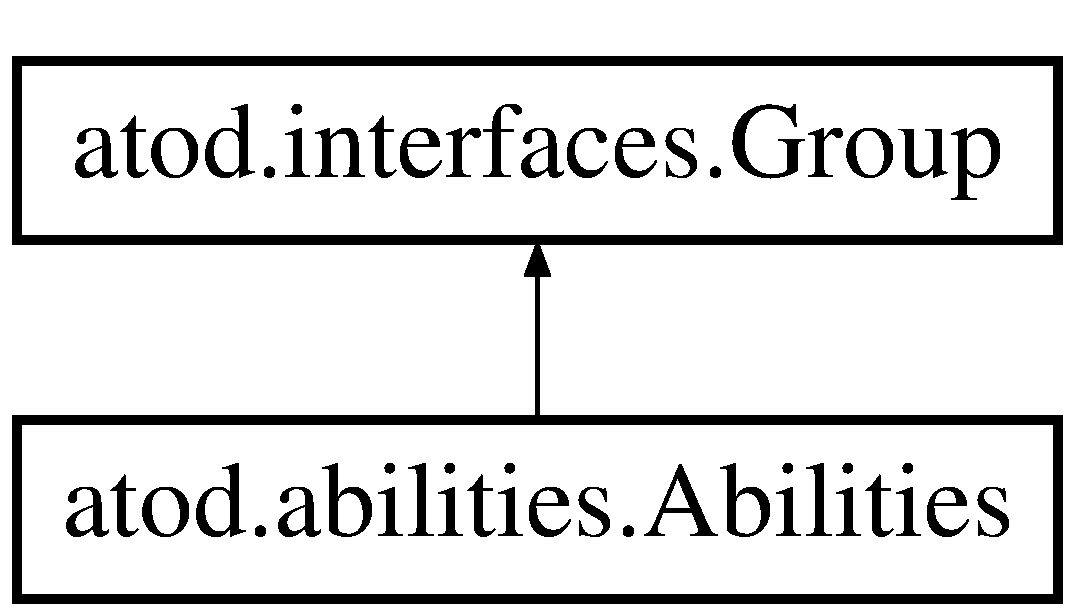
\includegraphics[height=2.000000cm]{classatod_1_1abilities_1_1_abilities}
\end{center}
\end{figure}
\subsection*{Public Member Functions}
\begin{DoxyCompactItemize}
\item 
def \hyperlink{classatod_1_1abilities_1_1_abilities_a1594c605444025644a197875b8b51faa}{from\+\_\+hero\+\_\+id} (cls, Hero\+ID)
\item 
def \hyperlink{classatod_1_1abilities_1_1_abilities_a097c69ffe687d823506a74aa18efc867}{all} (cls)
\item 
def \hyperlink{classatod_1_1abilities_1_1_abilities_aa86cdc4abf4ee615197c09dfb43300ca}{get\+\_\+list} (self)
\item 
def \hyperlink{classatod_1_1abilities_1_1_abilities_a815ad0f5d36d72298f2dffeb41d3dfc3}{get\+\_\+specs\+\_\+list} (self)
\item 
def \hyperlink{classatod_1_1abilities_1_1_abilities_a2cc0448d65e22ab6d9da0a784d0276c5}{get\+\_\+labels\+\_\+list} (self)
\item 
def \hyperlink{classatod_1_1abilities_1_1_abilities_a51f21a6496e8061f58f6de24c5e74ac5}{get\+\_\+texts} (self)
\item 
def \hyperlink{classatod_1_1abilities_1_1_abilities_a332197169464ae88a9251d36989b9876}{get\+\_\+summary} (self)
\end{DoxyCompactItemize}
\subsection*{Static Public Attributes}
\begin{DoxyCompactItemize}
\item 
{\bfseries member\+\_\+type} = \hyperlink{classatod_1_1abilities_1_1_ability}{Ability}\hypertarget{classatod_1_1abilities_1_1_abilities_ac16ab1be4985ec9cda43bddd3e34cece}{}\label{classatod_1_1abilities_1_1_abilities_ac16ab1be4985ec9cda43bddd3e34cece}

\end{DoxyCompactItemize}
\subsection*{Additional Inherited Members}


\subsection{Member Function Documentation}
\index{atod\+::abilities\+::\+Abilities@{atod\+::abilities\+::\+Abilities}!all@{all}}
\index{all@{all}!atod\+::abilities\+::\+Abilities@{atod\+::abilities\+::\+Abilities}}
\subsubsection[{\texorpdfstring{all(cls)}{all(cls)}}]{\setlength{\rightskip}{0pt plus 5cm}def atod.\+abilities.\+Abilities.\+all (
\begin{DoxyParamCaption}
\item[{}]{cls}
\end{DoxyParamCaption}
)}\hypertarget{classatod_1_1abilities_1_1_abilities_a097c69ffe687d823506a74aa18efc867}{}\label{classatod_1_1abilities_1_1_abilities_a097c69ffe687d823506a74aa18efc867}
\begin{DoxyVerb}Creates Abilities object with all heroes abilities in the game.\end{DoxyVerb}
 \index{atod\+::abilities\+::\+Abilities@{atod\+::abilities\+::\+Abilities}!from\+\_\+hero\+\_\+id@{from\+\_\+hero\+\_\+id}}
\index{from\+\_\+hero\+\_\+id@{from\+\_\+hero\+\_\+id}!atod\+::abilities\+::\+Abilities@{atod\+::abilities\+::\+Abilities}}
\subsubsection[{\texorpdfstring{from\+\_\+hero\+\_\+id(cls, Hero\+I\+D)}{from\_hero\_id(cls, HeroID)}}]{\setlength{\rightskip}{0pt plus 5cm}def atod.\+abilities.\+Abilities.\+from\+\_\+hero\+\_\+id (
\begin{DoxyParamCaption}
\item[{}]{cls, }
\item[{}]{Hero\+ID}
\end{DoxyParamCaption}
)}\hypertarget{classatod_1_1abilities_1_1_abilities_a1594c605444025644a197875b8b51faa}{}\label{classatod_1_1abilities_1_1_abilities_a1594c605444025644a197875b8b51faa}
\begin{DoxyVerb}Adds to members all abilities of the hero with `HeroID`. \end{DoxyVerb}
 \index{atod\+::abilities\+::\+Abilities@{atod\+::abilities\+::\+Abilities}!get\+\_\+labels\+\_\+list@{get\+\_\+labels\+\_\+list}}
\index{get\+\_\+labels\+\_\+list@{get\+\_\+labels\+\_\+list}!atod\+::abilities\+::\+Abilities@{atod\+::abilities\+::\+Abilities}}
\subsubsection[{\texorpdfstring{get\+\_\+labels\+\_\+list(self)}{get\_labels\_list(self)}}]{\setlength{\rightskip}{0pt plus 5cm}def atod.\+abilities.\+Abilities.\+get\+\_\+labels\+\_\+list (
\begin{DoxyParamCaption}
\item[{}]{self}
\end{DoxyParamCaption}
)}\hypertarget{classatod_1_1abilities_1_1_abilities_a2cc0448d65e22ab6d9da0a784d0276c5}{}\label{classatod_1_1abilities_1_1_abilities_a2cc0448d65e22ab6d9da0a784d0276c5}
\begin{DoxyVerb}Returns list of all member's descriptions (ONLY specs part). 

    Returns:
pd.DataFrame: shape=(len(members), len(<member description>)).
    Rows are abilities, columns - their properties.
    Labels columns names start with 'label_'.
\end{DoxyVerb}
 \index{atod\+::abilities\+::\+Abilities@{atod\+::abilities\+::\+Abilities}!get\+\_\+list@{get\+\_\+list}}
\index{get\+\_\+list@{get\+\_\+list}!atod\+::abilities\+::\+Abilities@{atod\+::abilities\+::\+Abilities}}
\subsubsection[{\texorpdfstring{get\+\_\+list(self)}{get\_list(self)}}]{\setlength{\rightskip}{0pt plus 5cm}def atod.\+abilities.\+Abilities.\+get\+\_\+list (
\begin{DoxyParamCaption}
\item[{}]{self}
\end{DoxyParamCaption}
)}\hypertarget{classatod_1_1abilities_1_1_abilities_aa86cdc4abf4ee615197c09dfb43300ca}{}\label{classatod_1_1abilities_1_1_abilities_aa86cdc4abf4ee615197c09dfb43300ca}
\begin{DoxyVerb}Returns information about members in the form: row is a member.
 
    'List' because descriptions are just concatenated with each other,
    but not summed by any means.

    Returns:
pd.DataFrame: shape=(len(self.members), 
    len(<member description>)). Rows are abilities, columns - 
    their properties. Labels columns names start with 
    'label_'.
\end{DoxyVerb}
 \index{atod\+::abilities\+::\+Abilities@{atod\+::abilities\+::\+Abilities}!get\+\_\+specs\+\_\+list@{get\+\_\+specs\+\_\+list}}
\index{get\+\_\+specs\+\_\+list@{get\+\_\+specs\+\_\+list}!atod\+::abilities\+::\+Abilities@{atod\+::abilities\+::\+Abilities}}
\subsubsection[{\texorpdfstring{get\+\_\+specs\+\_\+list(self)}{get\_specs\_list(self)}}]{\setlength{\rightskip}{0pt plus 5cm}def atod.\+abilities.\+Abilities.\+get\+\_\+specs\+\_\+list (
\begin{DoxyParamCaption}
\item[{}]{self}
\end{DoxyParamCaption}
)}\hypertarget{classatod_1_1abilities_1_1_abilities_a815ad0f5d36d72298f2dffeb41d3dfc3}{}\label{classatod_1_1abilities_1_1_abilities_a815ad0f5d36d72298f2dffeb41d3dfc3}
\begin{DoxyVerb}Returns list of all member's descriptions (ONLY specs part). 

    Returns:
pd.DataFrame: shape=(len(members), len(<member description>)).
    Rows are abilities, columns - their properties.
    Labels columns names start with 'label_'.
\end{DoxyVerb}
 \index{atod\+::abilities\+::\+Abilities@{atod\+::abilities\+::\+Abilities}!get\+\_\+summary@{get\+\_\+summary}}
\index{get\+\_\+summary@{get\+\_\+summary}!atod\+::abilities\+::\+Abilities@{atod\+::abilities\+::\+Abilities}}
\subsubsection[{\texorpdfstring{get\+\_\+summary(self)}{get\_summary(self)}}]{\setlength{\rightskip}{0pt plus 5cm}def atod.\+abilities.\+Abilities.\+get\+\_\+summary (
\begin{DoxyParamCaption}
\item[{}]{self}
\end{DoxyParamCaption}
)}\hypertarget{classatod_1_1abilities_1_1_abilities_a332197169464ae88a9251d36989b9876}{}\label{classatod_1_1abilities_1_1_abilities_a332197169464ae88a9251d36989b9876}
\begin{DoxyVerb}Sums up all labels of members (they are binary decoded).

    Returns:
pd.Series: 
\end{DoxyVerb}
 \index{atod\+::abilities\+::\+Abilities@{atod\+::abilities\+::\+Abilities}!get\+\_\+texts@{get\+\_\+texts}}
\index{get\+\_\+texts@{get\+\_\+texts}!atod\+::abilities\+::\+Abilities@{atod\+::abilities\+::\+Abilities}}
\subsubsection[{\texorpdfstring{get\+\_\+texts(self)}{get\_texts(self)}}]{\setlength{\rightskip}{0pt plus 5cm}def atod.\+abilities.\+Abilities.\+get\+\_\+texts (
\begin{DoxyParamCaption}
\item[{}]{self}
\end{DoxyParamCaption}
)}\hypertarget{classatod_1_1abilities_1_1_abilities_a51f21a6496e8061f58f6de24c5e74ac5}{}\label{classatod_1_1abilities_1_1_abilities_a51f21a6496e8061f58f6de24c5e74ac5}
\begin{DoxyVerb}Returns:
pd.DataFrame: texts of abilities in DataFrame.
\end{DoxyVerb}
 

The documentation for this class was generated from the following file\+:\begin{DoxyCompactItemize}
\item 
atod/abilities.\+py\end{DoxyCompactItemize}

\hypertarget{classabilities__old_1_1_abilities}{}\section{abilities\+\_\+old.\+Abilities Class Reference}
\label{classabilities__old_1_1_abilities}\index{abilities\+\_\+old.\+Abilities@{abilities\+\_\+old.\+Abilities}}
Inheritance diagram for abilities\+\_\+old.\+Abilities\+:\begin{figure}[H]
\begin{center}
\leavevmode
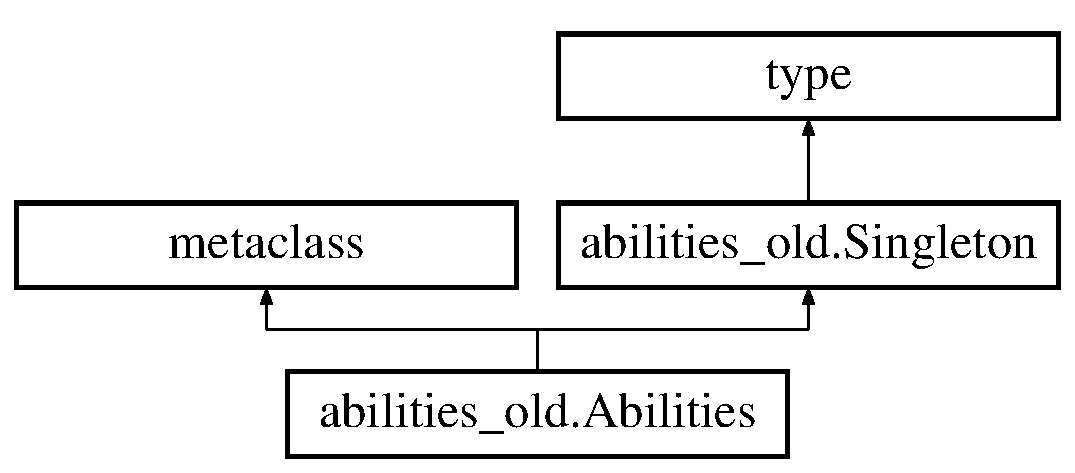
\includegraphics[height=3.000000cm]{classabilities__old_1_1_abilities}
\end{center}
\end{figure}
\subsection*{Public Member Functions}
\begin{DoxyCompactItemize}
\item 
def {\bfseries \+\_\+\+\_\+init\+\_\+\+\_\+} (self)\hypertarget{classabilities__old_1_1_abilities_a59973e3966bea9e4d94ce91e146ac53a}{}\label{classabilities__old_1_1_abilities_a59973e3966bea9e4d94ce91e146ac53a}

\item 
def {\bfseries find\+\_\+skills} (self)\hypertarget{classabilities__old_1_1_abilities_a2253e8f1ca1b7372486ba9d113a63ff3}{}\label{classabilities__old_1_1_abilities_a2253e8f1ca1b7372486ba9d113a63ff3}

\item 
def \hyperlink{classabilities__old_1_1_abilities_ac7ff3694fd993437f43fbd7879ed5474}{specials} (self)
\item 
def \hyperlink{classabilities__old_1_1_abilities_a4f7a8e97ac0c199a6a50998e4f8f2573}{raw} (self)
\item 
def {\bfseries skills\+\_\+list} (self)\hypertarget{classabilities__old_1_1_abilities_a98baf0ce9b1bad0a9e20840aa7bce02b}{}\label{classabilities__old_1_1_abilities_a98baf0ce9b1bad0a9e20840aa7bce02b}

\item 
def \hyperlink{classabilities__old_1_1_abilities_a6f4c7cce97440feefe4e5c0b655f00c6}{effects} (self)
\item 
def {\bfseries get\+\_\+properties} (self)\hypertarget{classabilities__old_1_1_abilities_a3ecc2429b98d449f4880f9cdfe202499}{}\label{classabilities__old_1_1_abilities_a3ecc2429b98d449f4880f9cdfe202499}

\item 
def \hyperlink{classabilities__old_1_1_abilities_a674c9327e5e6090a214ba86e6c817940}{encoding} (self)
\item 
def \hyperlink{classabilities__old_1_1_abilities_a4f4663563d1287a706f692935c9ee24f}{frame} (self)
\item 
def \hyperlink{classabilities__old_1_1_abilities_a372b29b8e75d50a58d1bd58eed5f2977}{clean\+\_\+frame} (self)
\item 
def \hyperlink{classabilities__old_1_1_abilities_a44f4974d12c407d669248fea33ffd363}{effects\+\_\+descriptions} (self)
\item 
def {\bfseries get\+\_\+cat\+\_\+variables} (self)\hypertarget{classabilities__old_1_1_abilities_aaa2b3db2fcb34301f01db6216bfda8fe}{}\label{classabilities__old_1_1_abilities_aaa2b3db2fcb34301f01db6216bfda8fe}

\item 
def \hyperlink{classabilities__old_1_1_abilities_aeb7d8464a0602ea1d4d609ce5768503c}{with\+\_\+property} (self, property\+\_\+)
\item 
def \hyperlink{classabilities__old_1_1_abilities_aabde6ec2cd2b12d2c4d4c80668bf33ef}{plot\+\_\+property} (self, property\+\_\+)
\item 
def \hyperlink{classabilities__old_1_1_abilities_a55c7dacd26fee941351455b7e4d6b7ee}{clustering\+\_\+by} (self, property\+\_\+)
\item 
def \hyperlink{classabilities__old_1_1_abilities_a82177be3ef5289b07d8ff7518aafcd53}{filter} (self, hero=\textquotesingle{}\textquotesingle{})
\item 
def \hyperlink{classabilities__old_1_1_abilities_adee377f2dfd5475c34dbc4f38a5b9986}{clean\+\_\+properties} (self)
\item 
def \hyperlink{classabilities__old_1_1_abilities_a076fa41cc24e0d38a60b6ac05d5bc71c}{load\+\_\+train\+\_\+test} (self)
\end{DoxyCompactItemize}
\subsection*{Public Attributes}
\begin{DoxyCompactItemize}
\item 
{\bfseries clean}\hypertarget{classabilities__old_1_1_abilities_a0a2945d4991378621525537d4d063213}{}\label{classabilities__old_1_1_abilities_a0a2945d4991378621525537d4d063213}

\item 
{\bfseries skills}\hypertarget{classabilities__old_1_1_abilities_a4ae268d5203f7c3764eb4e0416e76beb}{}\label{classabilities__old_1_1_abilities_a4ae268d5203f7c3764eb4e0416e76beb}

\item 
{\bfseries cat\+\_\+variables}\hypertarget{classabilities__old_1_1_abilities_ac50027edecd717d123c38b3743922407}{}\label{classabilities__old_1_1_abilities_ac50027edecd717d123c38b3743922407}

\item 
{\bfseries cat\+\_\+columns}\hypertarget{classabilities__old_1_1_abilities_aee9f9cc37afb798dc810928c9275a238}{}\label{classabilities__old_1_1_abilities_aee9f9cc37afb798dc810928c9275a238}

\end{DoxyCompactItemize}
\subsection*{Static Public Attributes}
\begin{DoxyCompactItemize}
\item 
list {\bfseries unused\+\_\+properties}
\end{DoxyCompactItemize}


\subsection{Detailed Description}
\begin{DoxyVerb}Singleton wrapper for npc_abilities.json.

    This class provides interface to work with abilities file.
    I'm using following definitions in the program:
        property    -- something that describes ability (e.g. cooldown)
        description -- all the properties of the ability
        skill       -- playable hero ability

    Attributes:
        _filename (str): absolute path to npc_abilities.json
        skills (dict)  : flatted skills from npc_abilities.json
\end{DoxyVerb}
 

\subsection{Member Function Documentation}
\index{abilities\+\_\+old\+::\+Abilities@{abilities\+\_\+old\+::\+Abilities}!clean\+\_\+frame@{clean\+\_\+frame}}
\index{clean\+\_\+frame@{clean\+\_\+frame}!abilities\+\_\+old\+::\+Abilities@{abilities\+\_\+old\+::\+Abilities}}
\subsubsection[{\texorpdfstring{clean\+\_\+frame(self)}{clean\_frame(self)}}]{\setlength{\rightskip}{0pt plus 5cm}def abilities\+\_\+old.\+Abilities.\+clean\+\_\+frame (
\begin{DoxyParamCaption}
\item[{}]{self}
\end{DoxyParamCaption}
)}\hypertarget{classabilities__old_1_1_abilities_a372b29b8e75d50a58d1bd58eed5f2977}{}\label{classabilities__old_1_1_abilities_a372b29b8e75d50a58d1bd58eed5f2977}
\begin{DoxyVerb}Function to call from outside of the module.

    Returns:
result_frame (pandas.DataFrame) : DataFrame of extracted vectors
\end{DoxyVerb}
 \index{abilities\+\_\+old\+::\+Abilities@{abilities\+\_\+old\+::\+Abilities}!clean\+\_\+properties@{clean\+\_\+properties}}
\index{clean\+\_\+properties@{clean\+\_\+properties}!abilities\+\_\+old\+::\+Abilities@{abilities\+\_\+old\+::\+Abilities}}
\subsubsection[{\texorpdfstring{clean\+\_\+properties(self)}{clean\_properties(self)}}]{\setlength{\rightskip}{0pt plus 5cm}def abilities\+\_\+old.\+Abilities.\+clean\+\_\+properties (
\begin{DoxyParamCaption}
\item[{}]{self}
\end{DoxyParamCaption}
)}\hypertarget{classabilities__old_1_1_abilities_adee377f2dfd5475c34dbc4f38a5b9986}{}\label{classabilities__old_1_1_abilities_adee377f2dfd5475c34dbc4f38a5b9986}
\begin{DoxyVerb}Removes parts of ability name from all the properties.

    There are a lot of skills which properties looks like this:
    <skillname>_<property>, they could be simplified to <property>.
    This function does exactly that.

    Returns:
clean (dict): cleaned skills dictionary, where every changed
    ability has special keyword `changed`.
\end{DoxyVerb}
 \index{abilities\+\_\+old\+::\+Abilities@{abilities\+\_\+old\+::\+Abilities}!clustering\+\_\+by@{clustering\+\_\+by}}
\index{clustering\+\_\+by@{clustering\+\_\+by}!abilities\+\_\+old\+::\+Abilities@{abilities\+\_\+old\+::\+Abilities}}
\subsubsection[{\texorpdfstring{clustering\+\_\+by(self, property\+\_\+)}{clustering\_by(self, property\_)}}]{\setlength{\rightskip}{0pt plus 5cm}def abilities\+\_\+old.\+Abilities.\+clustering\+\_\+by (
\begin{DoxyParamCaption}
\item[{}]{self, }
\item[{}]{property\+\_\+}
\end{DoxyParamCaption}
)}\hypertarget{classabilities__old_1_1_abilities_a55c7dacd26fee941351455b7e4d6b7ee}{}\label{classabilities__old_1_1_abilities_a55c7dacd26fee941351455b7e4d6b7ee}
\begin{DoxyVerb}Clusters abilities by given `property_`.

    Args:
property_ (str): property to cluster by

    Returns:
clusters (dict): maps skill to its cluster
\end{DoxyVerb}
 \index{abilities\+\_\+old\+::\+Abilities@{abilities\+\_\+old\+::\+Abilities}!effects@{effects}}
\index{effects@{effects}!abilities\+\_\+old\+::\+Abilities@{abilities\+\_\+old\+::\+Abilities}}
\subsubsection[{\texorpdfstring{effects(self)}{effects(self)}}]{\setlength{\rightskip}{0pt plus 5cm}def abilities\+\_\+old.\+Abilities.\+effects (
\begin{DoxyParamCaption}
\item[{}]{self}
\end{DoxyParamCaption}
)}\hypertarget{classabilities__old_1_1_abilities_a6f4c7cce97440feefe4e5c0b655f00c6}{}\label{classabilities__old_1_1_abilities_a6f4c7cce97440feefe4e5c0b655f00c6}
\begin{DoxyVerb}Returns:
(set): all words that occurs in abilities descriptions (keys)
\end{DoxyVerb}
 \index{abilities\+\_\+old\+::\+Abilities@{abilities\+\_\+old\+::\+Abilities}!effects\+\_\+descriptions@{effects\+\_\+descriptions}}
\index{effects\+\_\+descriptions@{effects\+\_\+descriptions}!abilities\+\_\+old\+::\+Abilities@{abilities\+\_\+old\+::\+Abilities}}
\subsubsection[{\texorpdfstring{effects\+\_\+descriptions(self)}{effects\_descriptions(self)}}]{\setlength{\rightskip}{0pt plus 5cm}def abilities\+\_\+old.\+Abilities.\+effects\+\_\+descriptions (
\begin{DoxyParamCaption}
\item[{}]{self}
\end{DoxyParamCaption}
)}\hypertarget{classabilities__old_1_1_abilities_a44f4974d12c407d669248fea33ffd363}{}\label{classabilities__old_1_1_abilities_a44f4974d12c407d669248fea33ffd363}
\begin{DoxyVerb}Generator of not categorical properties strings.

    Yields:
property_ (str): property where '_' replaced with ' '
\end{DoxyVerb}
 \index{abilities\+\_\+old\+::\+Abilities@{abilities\+\_\+old\+::\+Abilities}!encoding@{encoding}}
\index{encoding@{encoding}!abilities\+\_\+old\+::\+Abilities@{abilities\+\_\+old\+::\+Abilities}}
\subsubsection[{\texorpdfstring{encoding(self)}{encoding(self)}}]{\setlength{\rightskip}{0pt plus 5cm}def abilities\+\_\+old.\+Abilities.\+encoding (
\begin{DoxyParamCaption}
\item[{}]{self}
\end{DoxyParamCaption}
)}\hypertarget{classabilities__old_1_1_abilities_a674c9327e5e6090a214ba86e6c817940}{}\label{classabilities__old_1_1_abilities_a674c9327e5e6090a214ba86e6c817940}
\begin{DoxyVerb}Returns encoding of categorical features.\end{DoxyVerb}
 \index{abilities\+\_\+old\+::\+Abilities@{abilities\+\_\+old\+::\+Abilities}!filter@{filter}}
\index{filter@{filter}!abilities\+\_\+old\+::\+Abilities@{abilities\+\_\+old\+::\+Abilities}}
\subsubsection[{\texorpdfstring{filter(self, hero=\textquotesingle{}\textquotesingle{})}{filter(self, hero='')}}]{\setlength{\rightskip}{0pt plus 5cm}def abilities\+\_\+old.\+Abilities.\+filter (
\begin{DoxyParamCaption}
\item[{}]{self, }
\item[{}]{hero = {\ttfamily \textquotesingle{}\textquotesingle{}}}
\end{DoxyParamCaption}
)}\hypertarget{classabilities__old_1_1_abilities_a82177be3ef5289b07d8ff7518aafcd53}{}\label{classabilities__old_1_1_abilities_a82177be3ef5289b07d8ff7518aafcd53}
\begin{DoxyVerb}Returns all the hero abilities.

    Plan is to add more filtering options, for example cooldown,
    effects(armor, slow, damage...).

    Args:
hero (str): in game hero name
    (optional, default='')

    Returns:
abilities_ (list): list of Ability
\end{DoxyVerb}
 \index{abilities\+\_\+old\+::\+Abilities@{abilities\+\_\+old\+::\+Abilities}!frame@{frame}}
\index{frame@{frame}!abilities\+\_\+old\+::\+Abilities@{abilities\+\_\+old\+::\+Abilities}}
\subsubsection[{\texorpdfstring{frame(self)}{frame(self)}}]{\setlength{\rightskip}{0pt plus 5cm}def abilities\+\_\+old.\+Abilities.\+frame (
\begin{DoxyParamCaption}
\item[{}]{self}
\end{DoxyParamCaption}
)}\hypertarget{classabilities__old_1_1_abilities_a4f4663563d1287a706f692935c9ee24f}{}\label{classabilities__old_1_1_abilities_a4f4663563d1287a706f692935c9ee24f}
\begin{DoxyVerb}Function to call from outside of the module.

    Returns:
result_frame (pandas.DataFrame) : DataFrame of extracted vectors
\end{DoxyVerb}
 \index{abilities\+\_\+old\+::\+Abilities@{abilities\+\_\+old\+::\+Abilities}!load\+\_\+train\+\_\+test@{load\+\_\+train\+\_\+test}}
\index{load\+\_\+train\+\_\+test@{load\+\_\+train\+\_\+test}!abilities\+\_\+old\+::\+Abilities@{abilities\+\_\+old\+::\+Abilities}}
\subsubsection[{\texorpdfstring{load\+\_\+train\+\_\+test(self)}{load\_train\_test(self)}}]{\setlength{\rightskip}{0pt plus 5cm}def abilities\+\_\+old.\+Abilities.\+load\+\_\+train\+\_\+test (
\begin{DoxyParamCaption}
\item[{}]{self}
\end{DoxyParamCaption}
)}\hypertarget{classabilities__old_1_1_abilities_a076fa41cc24e0d38a60b6ac05d5bc71c}{}\label{classabilities__old_1_1_abilities_a076fa41cc24e0d38a60b6ac05d5bc71c}
\begin{DoxyVerb}Loads training and test data for classification.

    Returns:
X_train, y_train, X_test  of pd.DataFrame)
\end{DoxyVerb}
 \index{abilities\+\_\+old\+::\+Abilities@{abilities\+\_\+old\+::\+Abilities}!plot\+\_\+property@{plot\+\_\+property}}
\index{plot\+\_\+property@{plot\+\_\+property}!abilities\+\_\+old\+::\+Abilities@{abilities\+\_\+old\+::\+Abilities}}
\subsubsection[{\texorpdfstring{plot\+\_\+property(self, property\+\_\+)}{plot\_property(self, property\_)}}]{\setlength{\rightskip}{0pt plus 5cm}def abilities\+\_\+old.\+Abilities.\+plot\+\_\+property (
\begin{DoxyParamCaption}
\item[{}]{self, }
\item[{}]{property\+\_\+}
\end{DoxyParamCaption}
)}\hypertarget{classabilities__old_1_1_abilities_aabde6ec2cd2b12d2c4d4c80668bf33ef}{}\label{classabilities__old_1_1_abilities_aabde6ec2cd2b12d2c4d4c80668bf33ef}
\begin{DoxyVerb}Plots all values of given property with matplotlib.

    Args:
property_ (str): property to plot\end{DoxyVerb}
 \index{abilities\+\_\+old\+::\+Abilities@{abilities\+\_\+old\+::\+Abilities}!raw@{raw}}
\index{raw@{raw}!abilities\+\_\+old\+::\+Abilities@{abilities\+\_\+old\+::\+Abilities}}
\subsubsection[{\texorpdfstring{raw(self)}{raw(self)}}]{\setlength{\rightskip}{0pt plus 5cm}def abilities\+\_\+old.\+Abilities.\+raw (
\begin{DoxyParamCaption}
\item[{}]{self}
\end{DoxyParamCaption}
)}\hypertarget{classabilities__old_1_1_abilities_a4f7a8e97ac0c199a6a50998e4f8f2573}{}\label{classabilities__old_1_1_abilities_a4f7a8e97ac0c199a6a50998e4f8f2573}
\begin{DoxyVerb}Returns npc_abilities.txt as a dict.\end{DoxyVerb}
 \index{abilities\+\_\+old\+::\+Abilities@{abilities\+\_\+old\+::\+Abilities}!specials@{specials}}
\index{specials@{specials}!abilities\+\_\+old\+::\+Abilities@{abilities\+\_\+old\+::\+Abilities}}
\subsubsection[{\texorpdfstring{specials(self)}{specials(self)}}]{\setlength{\rightskip}{0pt plus 5cm}def abilities\+\_\+old.\+Abilities.\+specials (
\begin{DoxyParamCaption}
\item[{}]{self}
\end{DoxyParamCaption}
)}\hypertarget{classabilities__old_1_1_abilities_ac7ff3694fd993437f43fbd7879ed5474}{}\label{classabilities__old_1_1_abilities_ac7ff3694fd993437f43fbd7879ed5474}
\begin{DoxyVerb}Returns mapping ability -> AbilitySpecials without excluded.\end{DoxyVerb}
 \index{abilities\+\_\+old\+::\+Abilities@{abilities\+\_\+old\+::\+Abilities}!with\+\_\+property@{with\+\_\+property}}
\index{with\+\_\+property@{with\+\_\+property}!abilities\+\_\+old\+::\+Abilities@{abilities\+\_\+old\+::\+Abilities}}
\subsubsection[{\texorpdfstring{with\+\_\+property(self, property\+\_\+)}{with\_property(self, property\_)}}]{\setlength{\rightskip}{0pt plus 5cm}def abilities\+\_\+old.\+Abilities.\+with\+\_\+property (
\begin{DoxyParamCaption}
\item[{}]{self, }
\item[{}]{property\+\_\+}
\end{DoxyParamCaption}
)}\hypertarget{classabilities__old_1_1_abilities_aeb7d8464a0602ea1d4d609ce5768503c}{}\label{classabilities__old_1_1_abilities_aeb7d8464a0602ea1d4d609ce5768503c}
\begin{DoxyVerb}Finds properties which contain one of `keywords`.

    Args:
property_ (str): property to look in ability description keys

    Returns:
properties (dict): maps ability to its property value\end{DoxyVerb}
 

\subsection{Member Data Documentation}
\index{abilities\+\_\+old\+::\+Abilities@{abilities\+\_\+old\+::\+Abilities}!unused\+\_\+properties@{unused\+\_\+properties}}
\index{unused\+\_\+properties@{unused\+\_\+properties}!abilities\+\_\+old\+::\+Abilities@{abilities\+\_\+old\+::\+Abilities}}
\subsubsection[{\texorpdfstring{unused\+\_\+properties}{unused\_properties}}]{\setlength{\rightskip}{0pt plus 5cm}list abilities\+\_\+old.\+Abilities.\+unused\+\_\+properties\hspace{0.3cm}{\ttfamily [static]}}\hypertarget{classabilities__old_1_1_abilities_a76f031bc5ecabb1948635844ba0a3332}{}\label{classabilities__old_1_1_abilities_a76f031bc5ecabb1948635844ba0a3332}
{\bfseries Initial value\+:}
\begin{DoxyCode}
1 = [\textcolor{stringliteral}{'HasScepterUpgrade'}, \textcolor{stringliteral}{'LinkedSpecialBonus'},
2                          \textcolor{stringliteral}{'HotKeyOverride'}, \textcolor{stringliteral}{'levelkey'}, \textcolor{stringliteral}{'FightRecapLevel'},
3                          \textcolor{stringliteral}{'CalculateSpellDamageTooltip'}]
\end{DoxyCode}


The documentation for this class was generated from the following file\+:\begin{DoxyCompactItemize}
\item 
deprecated/abilities\+\_\+old.\+py\end{DoxyCompactItemize}

\hypertarget{classatod_1_1abilities_1_1_ability}{}\section{atod.\+abilities.\+Ability Class Reference}
\label{classatod_1_1abilities_1_1_ability}\index{atod.\+abilities.\+Ability@{atod.\+abilities.\+Ability}}
Inheritance diagram for atod.\+abilities.\+Ability\+:\begin{figure}[H]
\begin{center}
\leavevmode
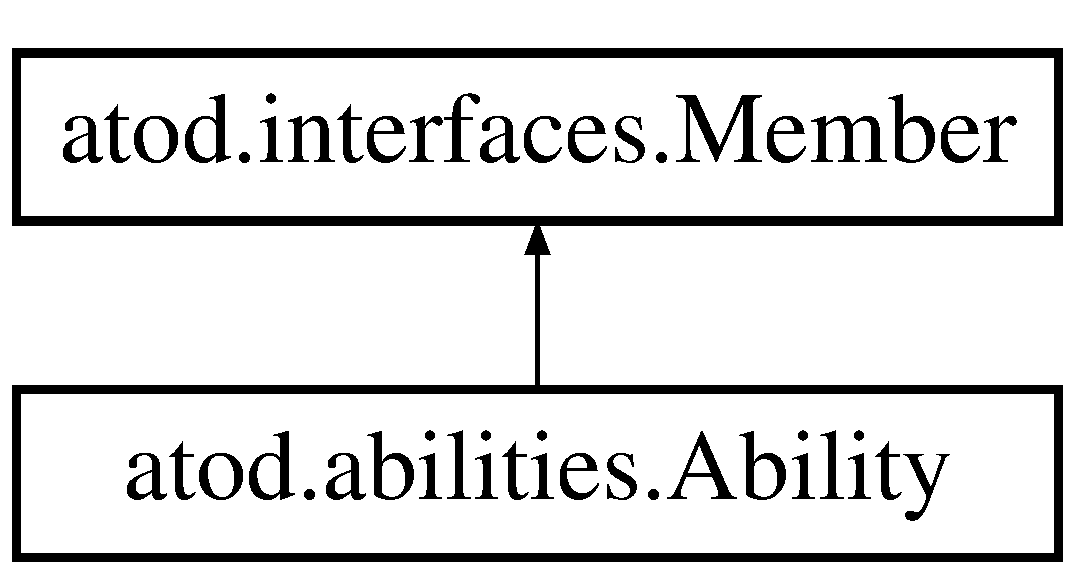
\includegraphics[height=2.000000cm]{classatod_1_1abilities_1_1_ability}
\end{center}
\end{figure}
\subsection*{Public Member Functions}
\begin{DoxyCompactItemize}
\item 
def {\bfseries \+\_\+\+\_\+init\+\_\+\+\_\+} (self, id\+\_\+, lvl=0)\hypertarget{classatod_1_1abilities_1_1_ability_a651ed69d665e42eb1bef757b4e524d7f}{}\label{classatod_1_1abilities_1_1_ability_a651ed69d665e42eb1bef757b4e524d7f}

\item 
def {\bfseries \+\_\+\+\_\+str\+\_\+\+\_\+} (self)\hypertarget{classatod_1_1abilities_1_1_ability_ae1af33d0f9e9f1773d7bf8d2e58aba3f}{}\label{classatod_1_1abilities_1_1_ability_ae1af33d0f9e9f1773d7bf8d2e58aba3f}

\item 
def {\bfseries \+\_\+\+\_\+repr\+\_\+\+\_\+} (self)\hypertarget{classatod_1_1abilities_1_1_ability_adbc62b463e3aece03e5ea5148c7866c1}{}\label{classatod_1_1abilities_1_1_ability_adbc62b463e3aece03e5ea5148c7866c1}

\item 
def \hyperlink{classatod_1_1abilities_1_1_ability_a79f3dd1154fb1862d396da4bb47eca85}{get\+\_\+description} (self)
\item 
def \hyperlink{classatod_1_1abilities_1_1_ability_a991ef8299a9817642bf457f7e8dd03b3}{get\+\_\+labels} (self)
\item 
def \hyperlink{classatod_1_1abilities_1_1_ability_af34b6c7240c2311edaffd784fb89cb4f}{get\+\_\+specs} (self)
\item 
def \hyperlink{classatod_1_1abilities_1_1_ability_a8ec6949a32f54ba31021fd710d525045}{get\+\_\+texts} (self)
\end{DoxyCompactItemize}
\subsection*{Public Attributes}
\begin{DoxyCompactItemize}
\item 
{\bfseries lvl}\hypertarget{classatod_1_1abilities_1_1_ability_ab87107b935627af4b9741545d1ce155a}{}\label{classatod_1_1abilities_1_1_ability_ab87107b935627af4b9741545d1ce155a}

\end{DoxyCompactItemize}
\subsection*{Static Public Attributes}
\begin{DoxyCompactItemize}
\item 
{\bfseries model} = Ability\+Model\hypertarget{classatod_1_1abilities_1_1_ability_ada4276561e99cca5a9b7ed604544218e}{}\label{classatod_1_1abilities_1_1_ability_ada4276561e99cca5a9b7ed604544218e}

\end{DoxyCompactItemize}


\subsection{Detailed Description}
\begin{DoxyVerb}Wrapper around Abilities data. \end{DoxyVerb}
 

\subsection{Member Function Documentation}
\index{atod\+::abilities\+::\+Ability@{atod\+::abilities\+::\+Ability}!get\+\_\+description@{get\+\_\+description}}
\index{get\+\_\+description@{get\+\_\+description}!atod\+::abilities\+::\+Ability@{atod\+::abilities\+::\+Ability}}
\subsubsection[{\texorpdfstring{get\+\_\+description(self)}{get\_description(self)}}]{\setlength{\rightskip}{0pt plus 5cm}def atod.\+abilities.\+Ability.\+get\+\_\+description (
\begin{DoxyParamCaption}
\item[{}]{self}
\end{DoxyParamCaption}
)}\hypertarget{classatod_1_1abilities_1_1_ability_a79f3dd1154fb1862d396da4bb47eca85}{}\label{classatod_1_1abilities_1_1_ability_a79f3dd1154fb1862d396da4bb47eca85}
\begin{DoxyVerb}Combines specs and labels in one description. \end{DoxyVerb}
 \index{atod\+::abilities\+::\+Ability@{atod\+::abilities\+::\+Ability}!get\+\_\+labels@{get\+\_\+labels}}
\index{get\+\_\+labels@{get\+\_\+labels}!atod\+::abilities\+::\+Ability@{atod\+::abilities\+::\+Ability}}
\subsubsection[{\texorpdfstring{get\+\_\+labels(self)}{get\_labels(self)}}]{\setlength{\rightskip}{0pt plus 5cm}def atod.\+abilities.\+Ability.\+get\+\_\+labels (
\begin{DoxyParamCaption}
\item[{}]{self}
\end{DoxyParamCaption}
)}\hypertarget{classatod_1_1abilities_1_1_ability_a991ef8299a9817642bf457f7e8dd03b3}{}\label{classatod_1_1abilities_1_1_ability_a991ef8299a9817642bf457f7e8dd03b3}
\begin{DoxyVerb}Returns labels of ability. \end{DoxyVerb}
 \index{atod\+::abilities\+::\+Ability@{atod\+::abilities\+::\+Ability}!get\+\_\+specs@{get\+\_\+specs}}
\index{get\+\_\+specs@{get\+\_\+specs}!atod\+::abilities\+::\+Ability@{atod\+::abilities\+::\+Ability}}
\subsubsection[{\texorpdfstring{get\+\_\+specs(self)}{get\_specs(self)}}]{\setlength{\rightskip}{0pt plus 5cm}def atod.\+abilities.\+Ability.\+get\+\_\+specs (
\begin{DoxyParamCaption}
\item[{}]{self}
\end{DoxyParamCaption}
)}\hypertarget{classatod_1_1abilities_1_1_ability_af34b6c7240c2311edaffd784fb89cb4f}{}\label{classatod_1_1abilities_1_1_ability_af34b6c7240c2311edaffd784fb89cb4f}
\begin{DoxyVerb}Returns specs of this ability. \end{DoxyVerb}
 \index{atod\+::abilities\+::\+Ability@{atod\+::abilities\+::\+Ability}!get\+\_\+texts@{get\+\_\+texts}}
\index{get\+\_\+texts@{get\+\_\+texts}!atod\+::abilities\+::\+Ability@{atod\+::abilities\+::\+Ability}}
\subsubsection[{\texorpdfstring{get\+\_\+texts(self)}{get\_texts(self)}}]{\setlength{\rightskip}{0pt plus 5cm}def atod.\+abilities.\+Ability.\+get\+\_\+texts (
\begin{DoxyParamCaption}
\item[{}]{self}
\end{DoxyParamCaption}
)}\hypertarget{classatod_1_1abilities_1_1_ability_a8ec6949a32f54ba31021fd710d525045}{}\label{classatod_1_1abilities_1_1_ability_a8ec6949a32f54ba31021fd710d525045}
\begin{DoxyVerb}Gets all the records in abilities_texts table for this ability.

    Returns:
pd.Series: index contain columns of abilities_texts table. 
    Can be empty, if this ability is not represented in texts
    table.
\end{DoxyVerb}
 

The documentation for this class was generated from the following file\+:\begin{DoxyCompactItemize}
\item 
atod/abilities.\+py\end{DoxyCompactItemize}

\hypertarget{classatod_1_1models_1_1ability_1_1_ability_model}{}\section{atod.\+models.\+ability.\+Ability\+Model Class Reference}
\label{classatod_1_1models_1_1ability_1_1_ability_model}\index{atod.\+models.\+ability.\+Ability\+Model@{atod.\+models.\+ability.\+Ability\+Model}}
Inheritance diagram for atod.\+models.\+ability.\+Ability\+Model\+:\begin{figure}[H]
\begin{center}
\leavevmode
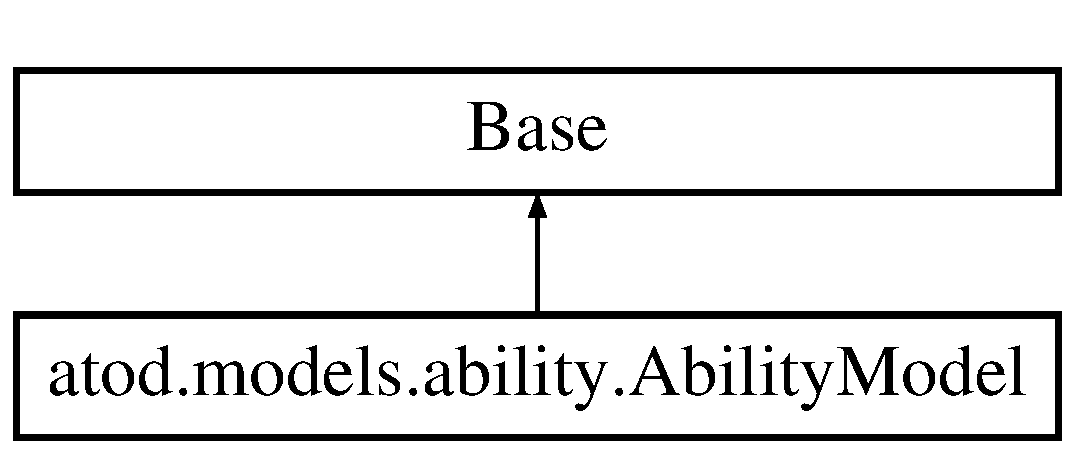
\includegraphics[height=2.000000cm]{classatod_1_1models_1_1ability_1_1_ability_model}
\end{center}
\end{figure}
\subsection*{Public Member Functions}
\begin{DoxyCompactItemize}
\item 
def {\bfseries \+\_\+\+\_\+init\+\_\+\+\_\+} (self, attrs)\hypertarget{classatod_1_1models_1_1ability_1_1_ability_model_a4c1c21db1fbba3b7d7ca49ef1f3db453}{}\label{classatod_1_1models_1_1ability_1_1_ability_model_a4c1c21db1fbba3b7d7ca49ef1f3db453}

\item 
def {\bfseries \+\_\+\+\_\+repr\+\_\+\+\_\+} (self)\hypertarget{classatod_1_1models_1_1ability_1_1_ability_model_a36437d1045c2ae3bf66f2c4190546d51}{}\label{classatod_1_1models_1_1ability_1_1_ability_model_a36437d1045c2ae3bf66f2c4190546d51}

\end{DoxyCompactItemize}
\subsection*{Public Attributes}
\begin{DoxyCompactItemize}
\item 
{\bfseries attrs}\hypertarget{classatod_1_1models_1_1ability_1_1_ability_model_ae0a27b3c720d313a5afb2e70064a718f}{}\label{classatod_1_1models_1_1ability_1_1_ability_model_ae0a27b3c720d313a5afb2e70064a718f}

\end{DoxyCompactItemize}


The documentation for this class was generated from the following file\+:\begin{DoxyCompactItemize}
\item 
atod/models/ability.\+py\end{DoxyCompactItemize}

\hypertarget{classatod_1_1models_1_1ability__specs_1_1_ability_specs_model}{}\section{atod.\+models.\+ability\+\_\+specs.\+Ability\+Specs\+Model Class Reference}
\label{classatod_1_1models_1_1ability__specs_1_1_ability_specs_model}\index{atod.\+models.\+ability\+\_\+specs.\+Ability\+Specs\+Model@{atod.\+models.\+ability\+\_\+specs.\+Ability\+Specs\+Model}}
Inheritance diagram for atod.\+models.\+ability\+\_\+specs.\+Ability\+Specs\+Model\+:\begin{figure}[H]
\begin{center}
\leavevmode
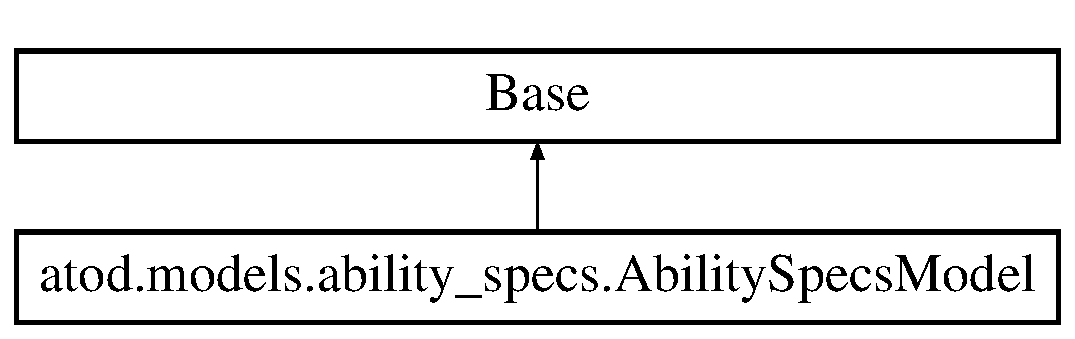
\includegraphics[height=2.000000cm]{classatod_1_1models_1_1ability__specs_1_1_ability_specs_model}
\end{center}
\end{figure}
\subsection*{Public Member Functions}
\begin{DoxyCompactItemize}
\item 
def {\bfseries \+\_\+\+\_\+init\+\_\+\+\_\+} (self, attrs)\hypertarget{classatod_1_1models_1_1ability__specs_1_1_ability_specs_model_aea44d80585948c298878ffa307569e8d}{}\label{classatod_1_1models_1_1ability__specs_1_1_ability_specs_model_aea44d80585948c298878ffa307569e8d}

\item 
def {\bfseries \+\_\+\+\_\+repr\+\_\+\+\_\+} (self)\hypertarget{classatod_1_1models_1_1ability__specs_1_1_ability_specs_model_af8b60a0f2f2b42840b6052045f629d21}{}\label{classatod_1_1models_1_1ability__specs_1_1_ability_specs_model_af8b60a0f2f2b42840b6052045f629d21}

\end{DoxyCompactItemize}
\subsection*{Public Attributes}
\begin{DoxyCompactItemize}
\item 
{\bfseries attrs}\hypertarget{classatod_1_1models_1_1ability__specs_1_1_ability_specs_model_a9fe9609e73c522edb83c871aa26fa3d9}{}\label{classatod_1_1models_1_1ability__specs_1_1_ability_specs_model_a9fe9609e73c522edb83c871aa26fa3d9}

\end{DoxyCompactItemize}


The documentation for this class was generated from the following file\+:\begin{DoxyCompactItemize}
\item 
atod/models/ability\+\_\+specs.\+py\end{DoxyCompactItemize}

\hypertarget{classatod_1_1models_1_1ability__texts_1_1_ability_texts_model}{}\section{atod.\+models.\+ability\+\_\+texts.\+Ability\+Texts\+Model Class Reference}
\label{classatod_1_1models_1_1ability__texts_1_1_ability_texts_model}\index{atod.\+models.\+ability\+\_\+texts.\+Ability\+Texts\+Model@{atod.\+models.\+ability\+\_\+texts.\+Ability\+Texts\+Model}}
Inheritance diagram for atod.\+models.\+ability\+\_\+texts.\+Ability\+Texts\+Model\+:\begin{figure}[H]
\begin{center}
\leavevmode
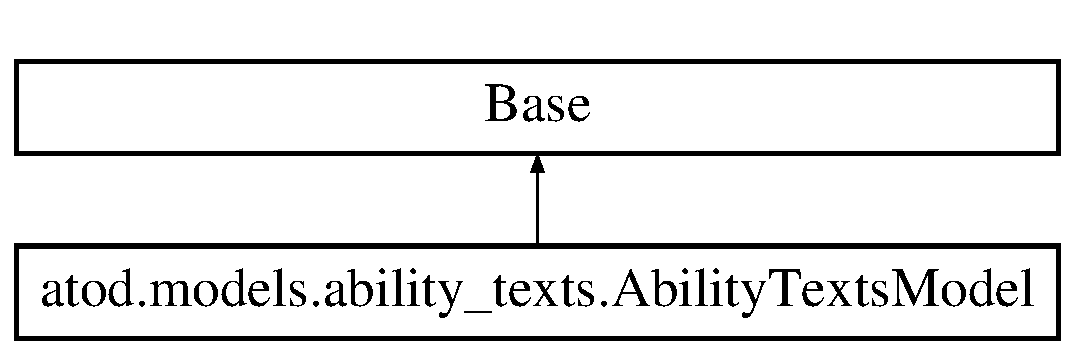
\includegraphics[height=2.000000cm]{classatod_1_1models_1_1ability__texts_1_1_ability_texts_model}
\end{center}
\end{figure}
\subsection*{Public Member Functions}
\begin{DoxyCompactItemize}
\item 
def {\bfseries \+\_\+\+\_\+init\+\_\+\+\_\+} (self, attrs)\hypertarget{classatod_1_1models_1_1ability__texts_1_1_ability_texts_model_ac7badf15d77512cbdf61481bdbdeb591}{}\label{classatod_1_1models_1_1ability__texts_1_1_ability_texts_model_ac7badf15d77512cbdf61481bdbdeb591}

\item 
def {\bfseries \+\_\+\+\_\+repr\+\_\+\+\_\+} (self)\hypertarget{classatod_1_1models_1_1ability__texts_1_1_ability_texts_model_ac10f7d190ef5dd2a23cbbfad8bf40301}{}\label{classatod_1_1models_1_1ability__texts_1_1_ability_texts_model_ac10f7d190ef5dd2a23cbbfad8bf40301}

\end{DoxyCompactItemize}
\subsection*{Public Attributes}
\begin{DoxyCompactItemize}
\item 
{\bfseries attrs}\hypertarget{classatod_1_1models_1_1ability__texts_1_1_ability_texts_model_ac6648f2410ed0592e010e167643ce1d8}{}\label{classatod_1_1models_1_1ability__texts_1_1_ability_texts_model_ac6648f2410ed0592e010e167643ce1d8}

\end{DoxyCompactItemize}
\subsection*{Static Public Attributes}
\begin{DoxyCompactItemize}
\item 
{\bfseries ID}
\item 
{\bfseries name} = Column(name=\textquotesingle{}name\textquotesingle{}, type\+\_\+=String)\hypertarget{classatod_1_1models_1_1ability__texts_1_1_ability_texts_model_a04571921f6292e0d35a24650cf4f6a11}{}\label{classatod_1_1models_1_1ability__texts_1_1_ability_texts_model_a04571921f6292e0d35a24650cf4f6a11}

\item 
{\bfseries lore} = Column(name=\textquotesingle{}lore\textquotesingle{}, type\+\_\+=String, nullable=True)\hypertarget{classatod_1_1models_1_1ability__texts_1_1_ability_texts_model_a082bdb6d4a069fbd169a20ac03471f4b}{}\label{classatod_1_1models_1_1ability__texts_1_1_ability_texts_model_a082bdb6d4a069fbd169a20ac03471f4b}

\item 
{\bfseries description} = Column(name=\textquotesingle{}description\textquotesingle{}, type\+\_\+=String)\hypertarget{classatod_1_1models_1_1ability__texts_1_1_ability_texts_model_ae1f5093bb5c78691ed472f2ed08f1375}{}\label{classatod_1_1models_1_1ability__texts_1_1_ability_texts_model_ae1f5093bb5c78691ed472f2ed08f1375}

\item 
{\bfseries notes} = Column(name=\textquotesingle{}notes\textquotesingle{}, type\+\_\+=String)\hypertarget{classatod_1_1models_1_1ability__texts_1_1_ability_texts_model_afac8692d6f07adf20ac92f3fa4f1b285}{}\label{classatod_1_1models_1_1ability__texts_1_1_ability_texts_model_afac8692d6f07adf20ac92f3fa4f1b285}

\item 
{\bfseries other} = Column(name=\textquotesingle{}other\textquotesingle{}, type\+\_\+=String, nullable=True)\hypertarget{classatod_1_1models_1_1ability__texts_1_1_ability_texts_model_ab53f1505cccef3d64e83e35919b43922}{}\label{classatod_1_1models_1_1ability__texts_1_1_ability_texts_model_ab53f1505cccef3d64e83e35919b43922}

\end{DoxyCompactItemize}


\subsection{Member Data Documentation}
\index{atod\+::models\+::ability\+\_\+texts\+::\+Ability\+Texts\+Model@{atod\+::models\+::ability\+\_\+texts\+::\+Ability\+Texts\+Model}!ID@{ID}}
\index{ID@{ID}!atod\+::models\+::ability\+\_\+texts\+::\+Ability\+Texts\+Model@{atod\+::models\+::ability\+\_\+texts\+::\+Ability\+Texts\+Model}}
\subsubsection[{\texorpdfstring{ID}{ID}}]{\setlength{\rightskip}{0pt plus 5cm}atod.\+models.\+ability\+\_\+texts.\+Ability\+Texts\+Model.\+ID\hspace{0.3cm}{\ttfamily [static]}}\hypertarget{classatod_1_1models_1_1ability__texts_1_1_ability_texts_model_a464cf4dba2a7e8fe3f9f5471622ab247}{}\label{classatod_1_1models_1_1ability__texts_1_1_ability_texts_model_a464cf4dba2a7e8fe3f9f5471622ab247}
{\bfseries Initial value\+:}
\begin{DoxyCode}
1 = Column(name=\textcolor{stringliteral}{'ID'}, type\_=Integer, primary\_key=\textcolor{keyword}{True},
2                          autoincrement=\textcolor{keyword}{False})
\end{DoxyCode}


The documentation for this class was generated from the following file\+:\begin{DoxyCompactItemize}
\item 
atod/models/ability\+\_\+texts.\+py\end{DoxyCompactItemize}

\hypertarget{classatod_1_1interfaces_1_1_group}{}\section{atod.\+interfaces.\+Group Class Reference}
\label{classatod_1_1interfaces_1_1_group}\index{atod.\+interfaces.\+Group@{atod.\+interfaces.\+Group}}
Inheritance diagram for atod.\+interfaces.\+Group\+:\begin{figure}[H]
\begin{center}
\leavevmode
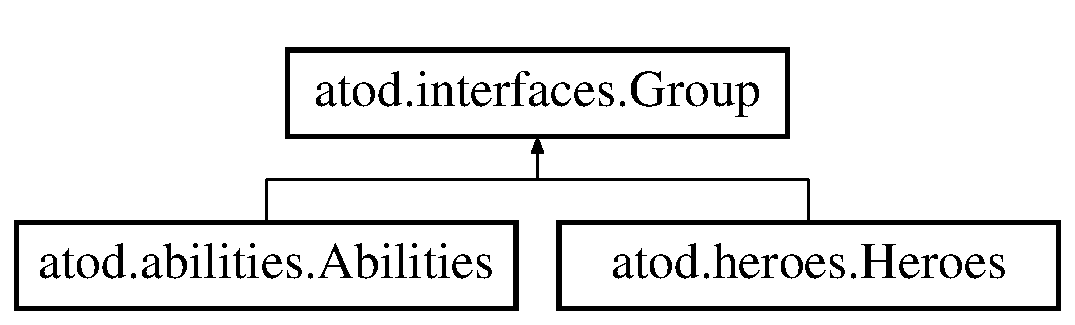
\includegraphics[height=2.000000cm]{classatod_1_1interfaces_1_1_group}
\end{center}
\end{figure}
\subsection*{Public Member Functions}
\begin{DoxyCompactItemize}
\item 
def {\bfseries \+\_\+\+\_\+init\+\_\+\+\_\+} (self, i\+\_\+members=\mbox{[}$\,$\mbox{]})\hypertarget{classatod_1_1interfaces_1_1_group_a42cd06857f6d9794d9314331c48d59bc}{}\label{classatod_1_1interfaces_1_1_group_a42cd06857f6d9794d9314331c48d59bc}

\item 
def {\bfseries add} (self, member)\hypertarget{classatod_1_1interfaces_1_1_group_a837162f848dea73b4fbb97fc43462096}{}\label{classatod_1_1interfaces_1_1_group_a837162f848dea73b4fbb97fc43462096}

\item 
def {\bfseries remove} (self, member\+\_\+name)\hypertarget{classatod_1_1interfaces_1_1_group_ac6ff24627bb35c20bdf53917db4ffccd}{}\label{classatod_1_1interfaces_1_1_group_ac6ff24627bb35c20bdf53917db4ffccd}

\item 
def \hyperlink{classatod_1_1interfaces_1_1_group_a5797ab75458b8a02fa05ba18415fc177}{compare} (self)
\item 
def \hyperlink{classatod_1_1interfaces_1_1_group_a024fa38236c8b271766bdfba3c426862}{get\+\_\+list} (self)
\item 
def \hyperlink{classatod_1_1interfaces_1_1_group_a4f8f899361148523842186e7822f6534}{get\+\_\+summary} (self)
\item 
def {\bfseries \+\_\+\+\_\+getitem\+\_\+\+\_\+} (self, item)\hypertarget{classatod_1_1interfaces_1_1_group_a79995ea461a23acd3eb633908a26aaca}{}\label{classatod_1_1interfaces_1_1_group_a79995ea461a23acd3eb633908a26aaca}

\item 
def {\bfseries \+\_\+\+\_\+len\+\_\+\+\_\+} (self)\hypertarget{classatod_1_1interfaces_1_1_group_adf5a671a4381821232ff047ed8ae19f3}{}\label{classatod_1_1interfaces_1_1_group_adf5a671a4381821232ff047ed8ae19f3}

\item 
def {\bfseries \+\_\+\+\_\+str\+\_\+\+\_\+} (self)\hypertarget{classatod_1_1interfaces_1_1_group_a85b3c25f20a5d8d355ee214ec90e911c}{}\label{classatod_1_1interfaces_1_1_group_a85b3c25f20a5d8d355ee214ec90e911c}

\end{DoxyCompactItemize}
\subsection*{Public Attributes}
\begin{DoxyCompactItemize}
\item 
{\bfseries members}\hypertarget{classatod_1_1interfaces_1_1_group_af72b66e3c59a9914f3d62d337386836a}{}\label{classatod_1_1interfaces_1_1_group_af72b66e3c59a9914f3d62d337386836a}

\end{DoxyCompactItemize}
\subsection*{Static Public Attributes}
\begin{DoxyCompactItemize}
\item 
{\bfseries member\+\_\+type} = None\hypertarget{classatod_1_1interfaces_1_1_group_a44890a5d53a0ac2bb6e033ee1ce480a3}{}\label{classatod_1_1interfaces_1_1_group_a44890a5d53a0ac2bb6e033ee1ce480a3}

\end{DoxyCompactItemize}


\subsection{Detailed Description}
\begin{DoxyVerb}Represents abstract set of members.

    Attributes:
        member_type (class): the type of member
        members (list)     : list of objects of class `member_type` 
\end{DoxyVerb}
 

\subsection{Member Function Documentation}
\index{atod\+::interfaces\+::\+Group@{atod\+::interfaces\+::\+Group}!compare@{compare}}
\index{compare@{compare}!atod\+::interfaces\+::\+Group@{atod\+::interfaces\+::\+Group}}
\subsubsection[{\texorpdfstring{compare(self)}{compare(self)}}]{\setlength{\rightskip}{0pt plus 5cm}def atod.\+interfaces.\+Group.\+compare (
\begin{DoxyParamCaption}
\item[{}]{self}
\end{DoxyParamCaption}
)}\hypertarget{classatod_1_1interfaces_1_1_group_a5797ab75458b8a02fa05ba18415fc177}{}\label{classatod_1_1interfaces_1_1_group_a5797ab75458b8a02fa05ba18415fc177}
\begin{DoxyVerb}Compare items. \end{DoxyVerb}
 \index{atod\+::interfaces\+::\+Group@{atod\+::interfaces\+::\+Group}!get\+\_\+list@{get\+\_\+list}}
\index{get\+\_\+list@{get\+\_\+list}!atod\+::interfaces\+::\+Group@{atod\+::interfaces\+::\+Group}}
\subsubsection[{\texorpdfstring{get\+\_\+list(self)}{get\_list(self)}}]{\setlength{\rightskip}{0pt plus 5cm}def atod.\+interfaces.\+Group.\+get\+\_\+list (
\begin{DoxyParamCaption}
\item[{}]{self}
\end{DoxyParamCaption}
)}\hypertarget{classatod_1_1interfaces_1_1_group_a024fa38236c8b271766bdfba3c426862}{}\label{classatod_1_1interfaces_1_1_group_a024fa38236c8b271766bdfba3c426862}
\begin{DoxyVerb}Combines all members in one data structure. \end{DoxyVerb}
 \index{atod\+::interfaces\+::\+Group@{atod\+::interfaces\+::\+Group}!get\+\_\+summary@{get\+\_\+summary}}
\index{get\+\_\+summary@{get\+\_\+summary}!atod\+::interfaces\+::\+Group@{atod\+::interfaces\+::\+Group}}
\subsubsection[{\texorpdfstring{get\+\_\+summary(self)}{get\_summary(self)}}]{\setlength{\rightskip}{0pt plus 5cm}def atod.\+interfaces.\+Group.\+get\+\_\+summary (
\begin{DoxyParamCaption}
\item[{}]{self}
\end{DoxyParamCaption}
)}\hypertarget{classatod_1_1interfaces_1_1_group_a4f8f899361148523842186e7822f6534}{}\label{classatod_1_1interfaces_1_1_group_a4f8f899361148523842186e7822f6534}
\begin{DoxyVerb}Adds properties of all the members and returns result. \end{DoxyVerb}
 

The documentation for this class was generated from the following file\+:\begin{DoxyCompactItemize}
\item 
atod/interfaces.\+py\end{DoxyCompactItemize}

\hypertarget{classhero_1_1_hero}{}\section{hero.\+Hero Class Reference}
\label{classhero_1_1_hero}\index{hero.\+Hero@{hero.\+Hero}}
Inheritance diagram for hero.\+Hero\+:\begin{figure}[H]
\begin{center}
\leavevmode
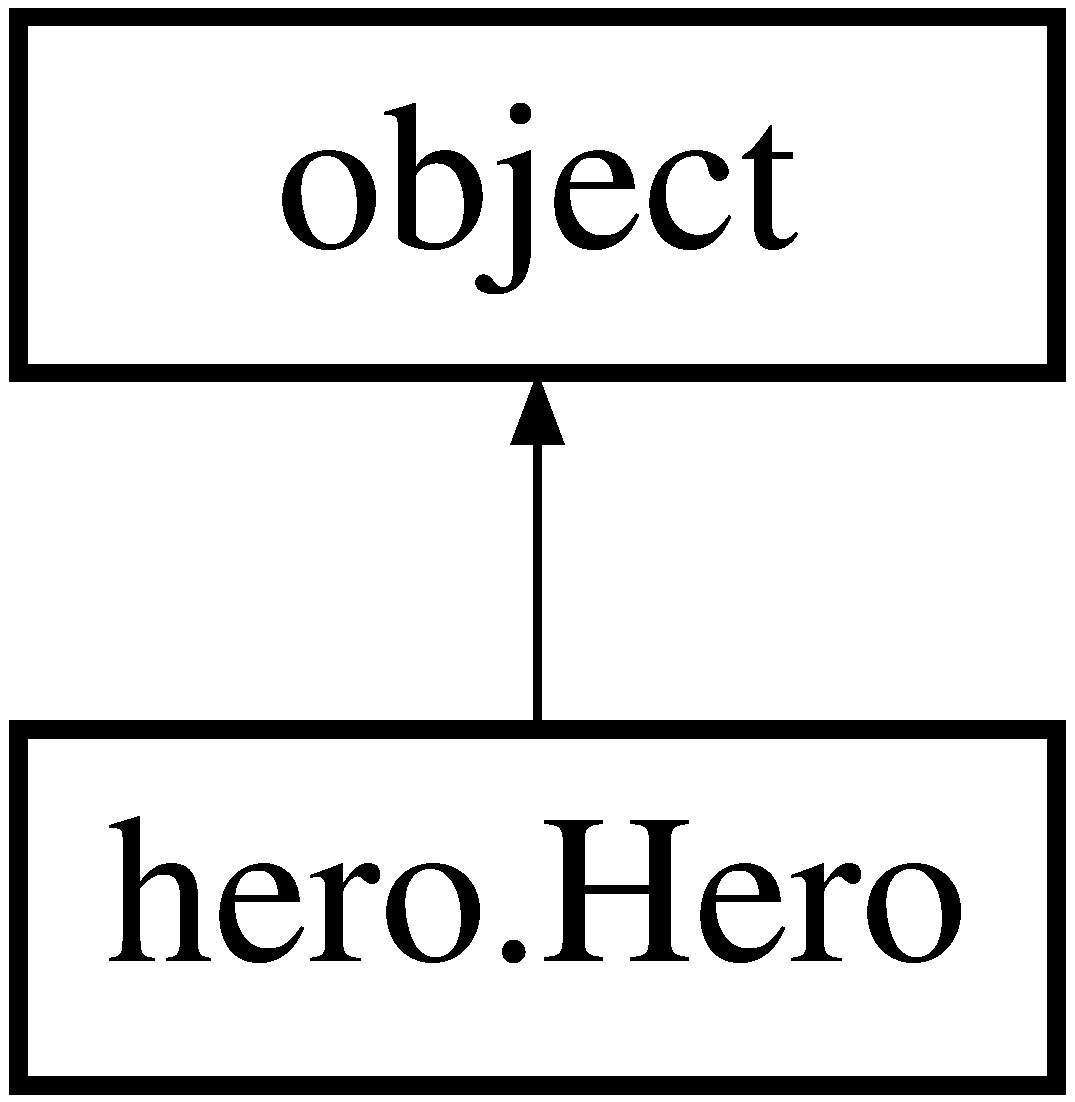
\includegraphics[height=2.000000cm]{classhero_1_1_hero}
\end{center}
\end{figure}
\subsection*{Public Member Functions}
\begin{DoxyCompactItemize}
\item 
def {\bfseries \+\_\+\+\_\+init\+\_\+\+\_\+} (self, arg)\hypertarget{classhero_1_1_hero_af248f7efb52f1b68da13533365e7808c}{}\label{classhero_1_1_hero_af248f7efb52f1b68da13533365e7808c}

\item 
def \hyperlink{classhero_1_1_hero_af015b2d88289932b884a27351f76ebda}{get\+\_\+features} (self, features\+\_\+dict)
\end{DoxyCompactItemize}
\subsection*{Public Attributes}
\begin{DoxyCompactItemize}
\item 
{\bfseries name}\hypertarget{classhero_1_1_hero_a9fd2ce620b7f00d3c51235a6ae68f6b1}{}\label{classhero_1_1_hero_a9fd2ce620b7f00d3c51235a6ae68f6b1}

\item 
{\bfseries hero\+\_\+id}\hypertarget{classhero_1_1_hero_ac6ab19abf39b947bb48d6f9c8d0327d8}{}\label{classhero_1_1_hero_ac6ab19abf39b947bb48d6f9c8d0327d8}

\item 
{\bfseries features}\hypertarget{classhero_1_1_hero_ae2955630410dde353e1776ac38ae4cc6}{}\label{classhero_1_1_hero_ae2955630410dde353e1776ac38ae4cc6}

\end{DoxyCompactItemize}


\subsection{Detailed Description}
\begin{DoxyVerb}Contain name and id, features of hero\end{DoxyVerb}
 

\subsection{Member Function Documentation}
\index{hero\+::\+Hero@{hero\+::\+Hero}!get\+\_\+features@{get\+\_\+features}}
\index{get\+\_\+features@{get\+\_\+features}!hero\+::\+Hero@{hero\+::\+Hero}}
\subsubsection[{\texorpdfstring{get\+\_\+features(self, features\+\_\+dict)}{get\_features(self, features\_dict)}}]{\setlength{\rightskip}{0pt plus 5cm}def hero.\+Hero.\+get\+\_\+features (
\begin{DoxyParamCaption}
\item[{}]{self, }
\item[{}]{features\+\_\+dict}
\end{DoxyParamCaption}
)}\hypertarget{classhero_1_1_hero_af015b2d88289932b884a27351f76ebda}{}\label{classhero_1_1_hero_af015b2d88289932b884a27351f76ebda}
\begin{DoxyVerb}Takes dict of features
Returns list of features for this hero
\end{DoxyVerb}
 

The documentation for this class was generated from the following file\+:\begin{DoxyCompactItemize}
\item 
deprecated/code/hero.\+py\end{DoxyCompactItemize}

\hypertarget{classatod_1_1heroes_1_1_hero}{}\section{atod.\+heroes.\+Hero Class Reference}
\label{classatod_1_1heroes_1_1_hero}\index{atod.\+heroes.\+Hero@{atod.\+heroes.\+Hero}}
Inheritance diagram for atod.\+heroes.\+Hero\+:\begin{figure}[H]
\begin{center}
\leavevmode
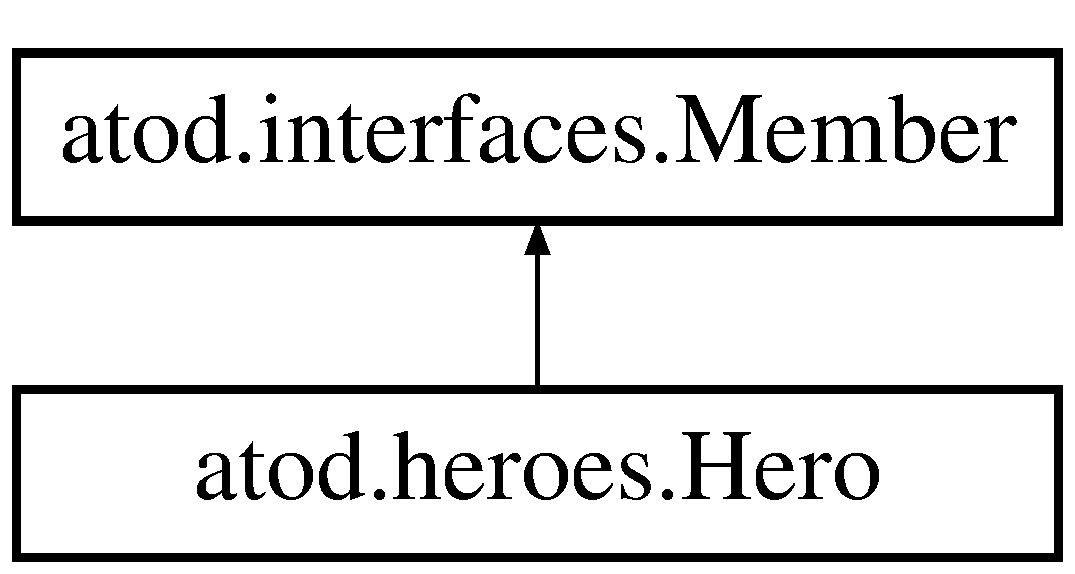
\includegraphics[height=2.000000cm]{classatod_1_1heroes_1_1_hero}
\end{center}
\end{figure}
\subsection*{Public Member Functions}
\begin{DoxyCompactItemize}
\item 
def {\bfseries \+\_\+\+\_\+init\+\_\+\+\_\+} (self, id\+\_\+, lvl=1)\hypertarget{classatod_1_1heroes_1_1_hero_a586daa470e18af152e442e70a594155b}{}\label{classatod_1_1heroes_1_1_hero_a586daa470e18af152e442e70a594155b}

\item 
def \hyperlink{classatod_1_1heroes_1_1_hero_ac2ba0862900a63e0a1f1d7a09111eb5f}{from\+\_\+name} (cls, name)
\item 
def {\bfseries get\+\_\+description} (self)\hypertarget{classatod_1_1heroes_1_1_hero_a830f17ec9fc71501b8bea6224814719f}{}\label{classatod_1_1heroes_1_1_hero_a830f17ec9fc71501b8bea6224814719f}

\item 
def {\bfseries str} (self)\hypertarget{classatod_1_1heroes_1_1_hero_ae64ab4c614f0131ffcc8d8fdfc4fc589}{}\label{classatod_1_1heroes_1_1_hero_ae64ab4c614f0131ffcc8d8fdfc4fc589}

\item 
def {\bfseries int} (self)\hypertarget{classatod_1_1heroes_1_1_hero_aacbd6a3822e3cf59cd4108c4ea38d9e1}{}\label{classatod_1_1heroes_1_1_hero_aacbd6a3822e3cf59cd4108c4ea38d9e1}

\item 
def {\bfseries agi} (self)\hypertarget{classatod_1_1heroes_1_1_hero_a267930ec44b1f9d9a389ec899775fddf}{}\label{classatod_1_1heroes_1_1_hero_a267930ec44b1f9d9a389ec899775fddf}

\item 
def {\bfseries health} (self)\hypertarget{classatod_1_1heroes_1_1_hero_a2deaa7c2b1e486817cdbfdb91903910f}{}\label{classatod_1_1heroes_1_1_hero_a2deaa7c2b1e486817cdbfdb91903910f}

\item 
def {\bfseries health\+\_\+regen} (self)\hypertarget{classatod_1_1heroes_1_1_hero_ad1ca633d554d2fe7910850049d204481}{}\label{classatod_1_1heroes_1_1_hero_ad1ca633d554d2fe7910850049d204481}

\item 
def {\bfseries mana} (self)\hypertarget{classatod_1_1heroes_1_1_hero_a9ccad513e9c5f0921b3d4fe6c3abaa85}{}\label{classatod_1_1heroes_1_1_hero_a9ccad513e9c5f0921b3d4fe6c3abaa85}

\item 
def {\bfseries mana\+\_\+regen} (self)\hypertarget{classatod_1_1heroes_1_1_hero_ad126237cdfa65a0207b960f55142f832}{}\label{classatod_1_1heroes_1_1_hero_ad126237cdfa65a0207b960f55142f832}

\item 
def {\bfseries armor} (self)\hypertarget{classatod_1_1heroes_1_1_hero_acf517ceebca484b42921ee00f98f0c49}{}\label{classatod_1_1heroes_1_1_hero_acf517ceebca484b42921ee00f98f0c49}

\item 
def {\bfseries \+\_\+\+\_\+str\+\_\+\+\_\+} (self)\hypertarget{classatod_1_1heroes_1_1_hero_a610f6f33addbb8771ffd78287f4b99af}{}\label{classatod_1_1heroes_1_1_hero_a610f6f33addbb8771ffd78287f4b99af}

\item 
def \hyperlink{classatod_1_1heroes_1_1_hero_ade8444c786bf0e7da8cbf6b8574a5f77}{get\+\_\+laning\+\_\+info} (self)
\item 
def \hyperlink{classatod_1_1heroes_1_1_hero_ac71de5b89c35ec14e61073797bfad23c}{get\+\_\+roles} (self)
\item 
def \hyperlink{classatod_1_1heroes_1_1_hero_acc769223b24b4bff2b260a6e6832b045}{get\+\_\+hero\+\_\+type} (self)
\end{DoxyCompactItemize}
\subsection*{Public Attributes}
\begin{DoxyCompactItemize}
\item 
{\bfseries in\+\_\+game\+\_\+name}\hypertarget{classatod_1_1heroes_1_1_hero_a96a8550c1b6971e88c9d0956e75ca85d}{}\label{classatod_1_1heroes_1_1_hero_a96a8550c1b6971e88c9d0956e75ca85d}

\item 
{\bfseries lvl}\hypertarget{classatod_1_1heroes_1_1_hero_a53719fc501a3b591f202e3adcdd7eaa6}{}\label{classatod_1_1heroes_1_1_hero_a53719fc501a3b591f202e3adcdd7eaa6}

\item 
{\bfseries specs}\hypertarget{classatod_1_1heroes_1_1_hero_abd6d76dcbabf512a87906417f0e59fbc}{}\label{classatod_1_1heroes_1_1_hero_abd6d76dcbabf512a87906417f0e59fbc}

\item 
{\bfseries abilities}\hypertarget{classatod_1_1heroes_1_1_hero_ae5cb5d96ba5716b131a0169b34cdf522}{}\label{classatod_1_1heroes_1_1_hero_ae5cb5d96ba5716b131a0169b34cdf522}

\end{DoxyCompactItemize}
\subsection*{Static Public Attributes}
\begin{DoxyCompactItemize}
\item 
int {\bfseries base\+\_\+health} = 200\hypertarget{classatod_1_1heroes_1_1_hero_a63d4617587f4729c7a55203b006a0690}{}\label{classatod_1_1heroes_1_1_hero_a63d4617587f4729c7a55203b006a0690}

\item 
float {\bfseries base\+\_\+health\+\_\+regen} = 0.\+25\hypertarget{classatod_1_1heroes_1_1_hero_a53c412a12d44420b4d01088e0c221ab1}{}\label{classatod_1_1heroes_1_1_hero_a53c412a12d44420b4d01088e0c221ab1}

\item 
int {\bfseries base\+\_\+mana} = 50\hypertarget{classatod_1_1heroes_1_1_hero_a62e40a1aeca72d4cf09703b70486b96f}{}\label{classatod_1_1heroes_1_1_hero_a62e40a1aeca72d4cf09703b70486b96f}

\item 
float {\bfseries base\+\_\+mana\+\_\+regen} = 0.\+01\hypertarget{classatod_1_1heroes_1_1_hero_addf105e6717aa8562ef413bd23fa1b33}{}\label{classatod_1_1heroes_1_1_hero_addf105e6717aa8562ef413bd23fa1b33}

\item 
int {\bfseries base\+\_\+damage} = 21\hypertarget{classatod_1_1heroes_1_1_hero_a2ca0e9cedc05db0dda44c0d6738b2016}{}\label{classatod_1_1heroes_1_1_hero_a2ca0e9cedc05db0dda44c0d6738b2016}

\item 
int {\bfseries base\+\_\+armor} = -\/1\hypertarget{classatod_1_1heroes_1_1_hero_ae4828f969afb8590a8df38f54fc2dc2a}{}\label{classatod_1_1heroes_1_1_hero_ae4828f969afb8590a8df38f54fc2dc2a}

\end{DoxyCompactItemize}


\subsection{Detailed Description}
\begin{DoxyVerb}Interface for HeroModel. \end{DoxyVerb}
 

\subsection{Member Function Documentation}
\index{atod\+::heroes\+::\+Hero@{atod\+::heroes\+::\+Hero}!from\+\_\+name@{from\+\_\+name}}
\index{from\+\_\+name@{from\+\_\+name}!atod\+::heroes\+::\+Hero@{atod\+::heroes\+::\+Hero}}
\subsubsection[{\texorpdfstring{from\+\_\+name(cls, name)}{from\_name(cls, name)}}]{\setlength{\rightskip}{0pt plus 5cm}def atod.\+heroes.\+Hero.\+from\+\_\+name (
\begin{DoxyParamCaption}
\item[{}]{cls, }
\item[{}]{name}
\end{DoxyParamCaption}
)}\hypertarget{classatod_1_1heroes_1_1_hero_ac2ba0862900a63e0a1f1d7a09111eb5f}{}\label{classatod_1_1heroes_1_1_hero_ac2ba0862900a63e0a1f1d7a09111eb5f}
\begin{DoxyVerb}Converts name to id with and calls init. 

    Raises:
ValueError: if `name` is not in heroes.name column
\end{DoxyVerb}
 \index{atod\+::heroes\+::\+Hero@{atod\+::heroes\+::\+Hero}!get\+\_\+hero\+\_\+type@{get\+\_\+hero\+\_\+type}}
\index{get\+\_\+hero\+\_\+type@{get\+\_\+hero\+\_\+type}!atod\+::heroes\+::\+Hero@{atod\+::heroes\+::\+Hero}}
\subsubsection[{\texorpdfstring{get\+\_\+hero\+\_\+type(self)}{get\_hero\_type(self)}}]{\setlength{\rightskip}{0pt plus 5cm}def atod.\+heroes.\+Hero.\+get\+\_\+hero\+\_\+type (
\begin{DoxyParamCaption}
\item[{}]{self}
\end{DoxyParamCaption}
)}\hypertarget{classatod_1_1heroes_1_1_hero_acc769223b24b4bff2b260a6e6832b045}{}\label{classatod_1_1heroes_1_1_hero_acc769223b24b4bff2b260a6e6832b045}
\begin{DoxyVerb}Returns:
pd.Series: laning info of this hero.

    Notes:
The latest heroes does not have this field, so Series filled
with zeroes would be returned.
\end{DoxyVerb}
 \index{atod\+::heroes\+::\+Hero@{atod\+::heroes\+::\+Hero}!get\+\_\+laning\+\_\+info@{get\+\_\+laning\+\_\+info}}
\index{get\+\_\+laning\+\_\+info@{get\+\_\+laning\+\_\+info}!atod\+::heroes\+::\+Hero@{atod\+::heroes\+::\+Hero}}
\subsubsection[{\texorpdfstring{get\+\_\+laning\+\_\+info(self)}{get\_laning\_info(self)}}]{\setlength{\rightskip}{0pt plus 5cm}def atod.\+heroes.\+Hero.\+get\+\_\+laning\+\_\+info (
\begin{DoxyParamCaption}
\item[{}]{self}
\end{DoxyParamCaption}
)}\hypertarget{classatod_1_1heroes_1_1_hero_ade8444c786bf0e7da8cbf6b8574a5f77}{}\label{classatod_1_1heroes_1_1_hero_ade8444c786bf0e7da8cbf6b8574a5f77}
\begin{DoxyVerb}Returns:
pd.Series: laning info of this hero.

    Notes:
The latest heroes does not have this field, so Series filled
with zeroes would be returned.
\end{DoxyVerb}
 \index{atod\+::heroes\+::\+Hero@{atod\+::heroes\+::\+Hero}!get\+\_\+roles@{get\+\_\+roles}}
\index{get\+\_\+roles@{get\+\_\+roles}!atod\+::heroes\+::\+Hero@{atod\+::heroes\+::\+Hero}}
\subsubsection[{\texorpdfstring{get\+\_\+roles(self)}{get\_roles(self)}}]{\setlength{\rightskip}{0pt plus 5cm}def atod.\+heroes.\+Hero.\+get\+\_\+roles (
\begin{DoxyParamCaption}
\item[{}]{self}
\end{DoxyParamCaption}
)}\hypertarget{classatod_1_1heroes_1_1_hero_ac71de5b89c35ec14e61073797bfad23c}{}\label{classatod_1_1heroes_1_1_hero_ac71de5b89c35ec14e61073797bfad23c}
\begin{DoxyVerb}Returns:
pd.Series: roles levels of this hero.

    Notes:
The latest heroes does not have this field, so Series filled
with zeroes would be returned.
\end{DoxyVerb}
 

The documentation for this class was generated from the following file\+:\begin{DoxyCompactItemize}
\item 
atod/heroes.\+py\end{DoxyCompactItemize}

\hypertarget{classatod_1_1heroes_1_1_heroes}{}\section{atod.\+heroes.\+Heroes Class Reference}
\label{classatod_1_1heroes_1_1_heroes}\index{atod.\+heroes.\+Heroes@{atod.\+heroes.\+Heroes}}
Inheritance diagram for atod.\+heroes.\+Heroes\+:\begin{figure}[H]
\begin{center}
\leavevmode
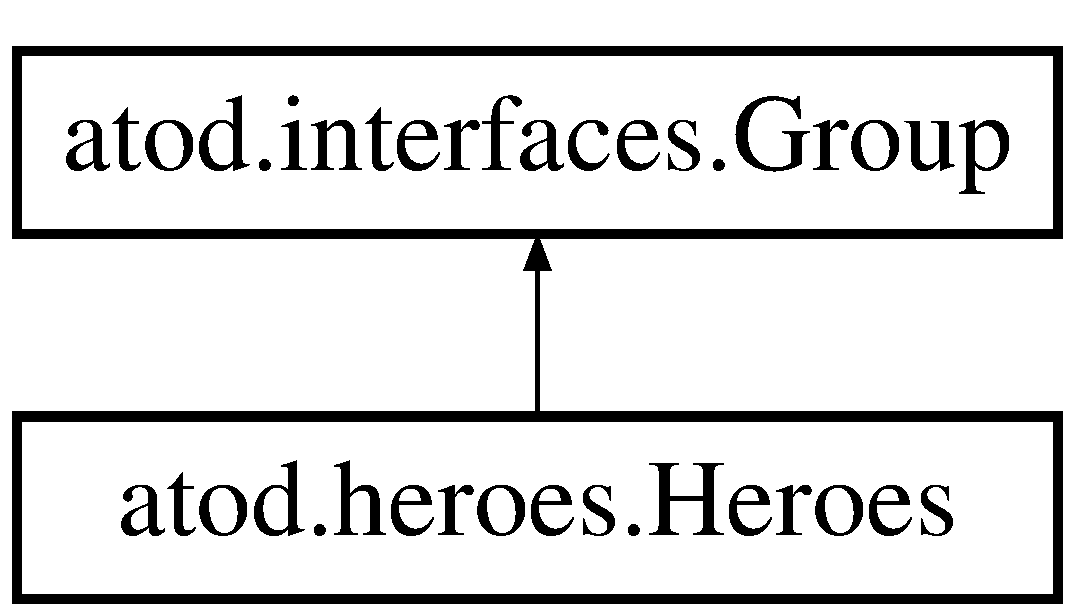
\includegraphics[height=2.000000cm]{classatod_1_1heroes_1_1_heroes}
\end{center}
\end{figure}
\subsection*{Public Member Functions}
\begin{DoxyCompactItemize}
\item 
def \hyperlink{classatod_1_1heroes_1_1_heroes_ab33167d6a3af098c9e055a83e271fc7f}{get\+\_\+summary} (self)
\item 
def \hyperlink{classatod_1_1heroes_1_1_heroes_a71cda232697372e876599e2a51df5b23}{all} (cls)
\end{DoxyCompactItemize}
\subsection*{Static Public Attributes}
\begin{DoxyCompactItemize}
\item 
{\bfseries member\+\_\+type} = \hyperlink{classatod_1_1heroes_1_1_hero}{Hero}\hypertarget{classatod_1_1heroes_1_1_heroes_a91f57a9b49cf151cb96af681f0798d19}{}\label{classatod_1_1heroes_1_1_heroes_a91f57a9b49cf151cb96af681f0798d19}

\end{DoxyCompactItemize}
\subsection*{Additional Inherited Members}


\subsection{Member Function Documentation}
\index{atod\+::heroes\+::\+Heroes@{atod\+::heroes\+::\+Heroes}!all@{all}}
\index{all@{all}!atod\+::heroes\+::\+Heroes@{atod\+::heroes\+::\+Heroes}}
\subsubsection[{\texorpdfstring{all(cls)}{all(cls)}}]{\setlength{\rightskip}{0pt plus 5cm}def atod.\+heroes.\+Heroes.\+all (
\begin{DoxyParamCaption}
\item[{}]{cls}
\end{DoxyParamCaption}
)}\hypertarget{classatod_1_1heroes_1_1_heroes_a71cda232697372e876599e2a51df5b23}{}\label{classatod_1_1heroes_1_1_heroes_a71cda232697372e876599e2a51df5b23}
\begin{DoxyVerb}Creates Abilities object with all heroes abilities in the game.\end{DoxyVerb}
 \index{atod\+::heroes\+::\+Heroes@{atod\+::heroes\+::\+Heroes}!get\+\_\+summary@{get\+\_\+summary}}
\index{get\+\_\+summary@{get\+\_\+summary}!atod\+::heroes\+::\+Heroes@{atod\+::heroes\+::\+Heroes}}
\subsubsection[{\texorpdfstring{get\+\_\+summary(self)}{get\_summary(self)}}]{\setlength{\rightskip}{0pt plus 5cm}def atod.\+heroes.\+Heroes.\+get\+\_\+summary (
\begin{DoxyParamCaption}
\item[{}]{self}
\end{DoxyParamCaption}
)}\hypertarget{classatod_1_1heroes_1_1_heroes_ab33167d6a3af098c9e055a83e271fc7f}{}\label{classatod_1_1heroes_1_1_heroes_ab33167d6a3af098c9e055a83e271fc7f}
\begin{DoxyVerb}Sums up numeric properties, encodes and sums up categorical. \end{DoxyVerb}
 

The documentation for this class was generated from the following file\+:\begin{DoxyCompactItemize}
\item 
atod/heroes.\+py\end{DoxyCompactItemize}

\hypertarget{classatod_1_1models_1_1hero_1_1_hero_model}{}\section{atod.\+models.\+hero.\+Hero\+Model Class Reference}
\label{classatod_1_1models_1_1hero_1_1_hero_model}\index{atod.\+models.\+hero.\+Hero\+Model@{atod.\+models.\+hero.\+Hero\+Model}}
Inheritance diagram for atod.\+models.\+hero.\+Hero\+Model\+:\begin{figure}[H]
\begin{center}
\leavevmode
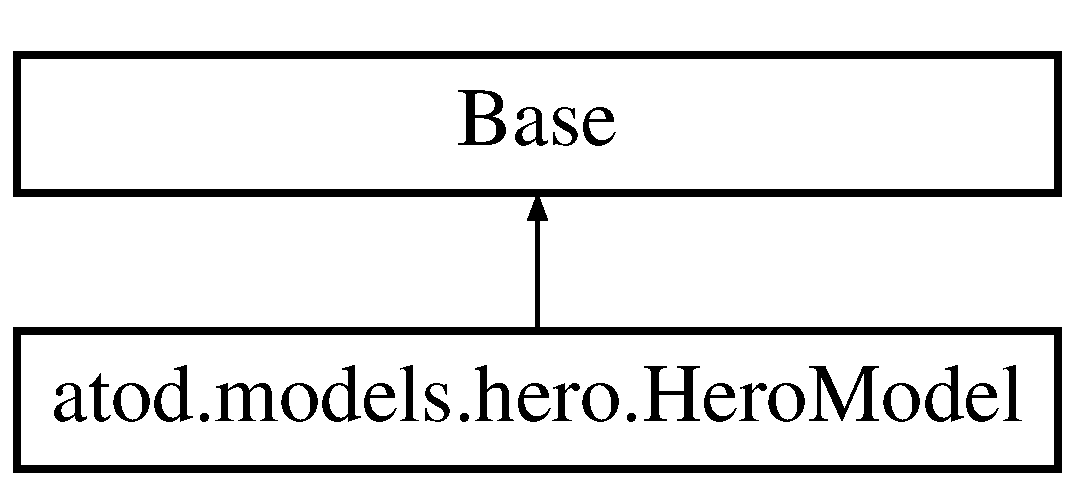
\includegraphics[height=2.000000cm]{classatod_1_1models_1_1hero_1_1_hero_model}
\end{center}
\end{figure}
\subsection*{Public Member Functions}
\begin{DoxyCompactItemize}
\item 
def {\bfseries \+\_\+\+\_\+init\+\_\+\+\_\+} (self, attrs)\hypertarget{classatod_1_1models_1_1hero_1_1_hero_model_a2dbdaab336ce65033f13e21586d3c9c2}{}\label{classatod_1_1models_1_1hero_1_1_hero_model_a2dbdaab336ce65033f13e21586d3c9c2}

\item 
def {\bfseries \+\_\+\+\_\+repr\+\_\+\+\_\+} (self)\hypertarget{classatod_1_1models_1_1hero_1_1_hero_model_ab231395fb3d47764d3924aa9f300d6e0}{}\label{classatod_1_1models_1_1hero_1_1_hero_model_ab231395fb3d47764d3924aa9f300d6e0}

\end{DoxyCompactItemize}
\subsection*{Public Attributes}
\begin{DoxyCompactItemize}
\item 
{\bfseries attrs}\hypertarget{classatod_1_1models_1_1hero_1_1_hero_model_a10c17b5904721748f3759b46ecd00ebb}{}\label{classatod_1_1models_1_1hero_1_1_hero_model_a10c17b5904721748f3759b46ecd00ebb}

\end{DoxyCompactItemize}
\subsection*{Static Public Attributes}
\begin{DoxyCompactItemize}
\item 
tuple {\bfseries heroes} = (Column($\ast$$\ast$col) for col in get\+\_\+heroes\+\_\+schema())\hypertarget{classatod_1_1models_1_1hero_1_1_hero_model_acb4b61406491bf4a3962821a75e66022}{}\label{classatod_1_1models_1_1hero_1_1_hero_model_acb4b61406491bf4a3962821a75e66022}

\end{DoxyCompactItemize}


The documentation for this class was generated from the following file\+:\begin{DoxyCompactItemize}
\item 
atod/models/hero.\+py\end{DoxyCompactItemize}

\hypertarget{classatod_1_1models_1_1item_1_1_item_model}{}\section{atod.\+models.\+item.\+Item\+Model Class Reference}
\label{classatod_1_1models_1_1item_1_1_item_model}\index{atod.\+models.\+item.\+Item\+Model@{atod.\+models.\+item.\+Item\+Model}}
Inheritance diagram for atod.\+models.\+item.\+Item\+Model\+:\begin{figure}[H]
\begin{center}
\leavevmode
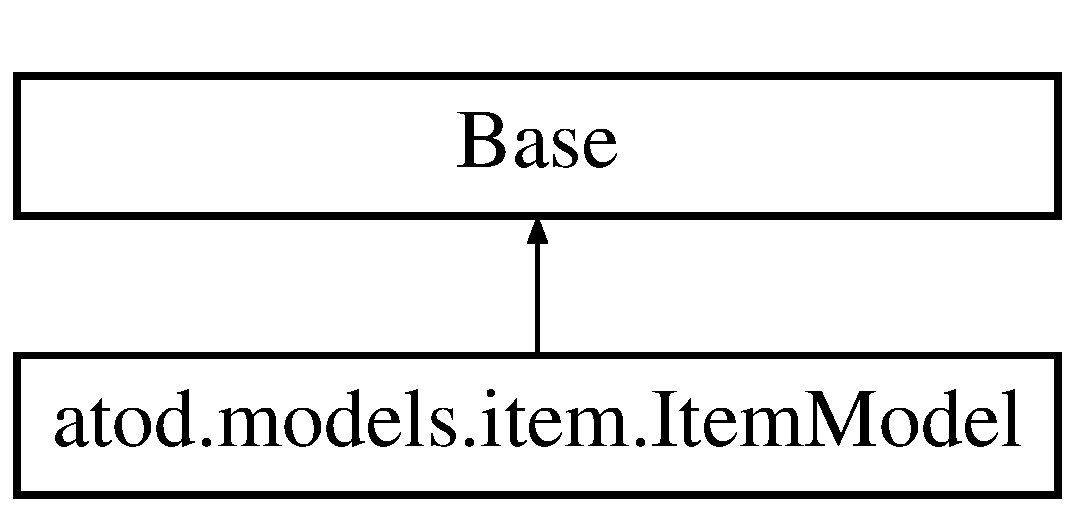
\includegraphics[height=2.000000cm]{classatod_1_1models_1_1item_1_1_item_model}
\end{center}
\end{figure}
\subsection*{Public Member Functions}
\begin{DoxyCompactItemize}
\item 
def {\bfseries \+\_\+\+\_\+init\+\_\+\+\_\+} (self, attrs)\hypertarget{classatod_1_1models_1_1item_1_1_item_model_afc641e705e3b63c23a40011bcf93c2a8}{}\label{classatod_1_1models_1_1item_1_1_item_model_afc641e705e3b63c23a40011bcf93c2a8}

\item 
def {\bfseries \+\_\+\+\_\+repr\+\_\+\+\_\+} (self)\hypertarget{classatod_1_1models_1_1item_1_1_item_model_af8fedb7b227633ef4ef5e28ef710e357}{}\label{classatod_1_1models_1_1item_1_1_item_model_af8fedb7b227633ef4ef5e28ef710e357}

\end{DoxyCompactItemize}


The documentation for this class was generated from the following file\+:\begin{DoxyCompactItemize}
\item 
atod/models/item.\+py\end{DoxyCompactItemize}

\hypertarget{classleague_1_1_league}{}\section{league.\+League Class Reference}
\label{classleague_1_1_league}\index{league.\+League@{league.\+League}}
Inheritance diagram for league.\+League\+:\begin{figure}[H]
\begin{center}
\leavevmode
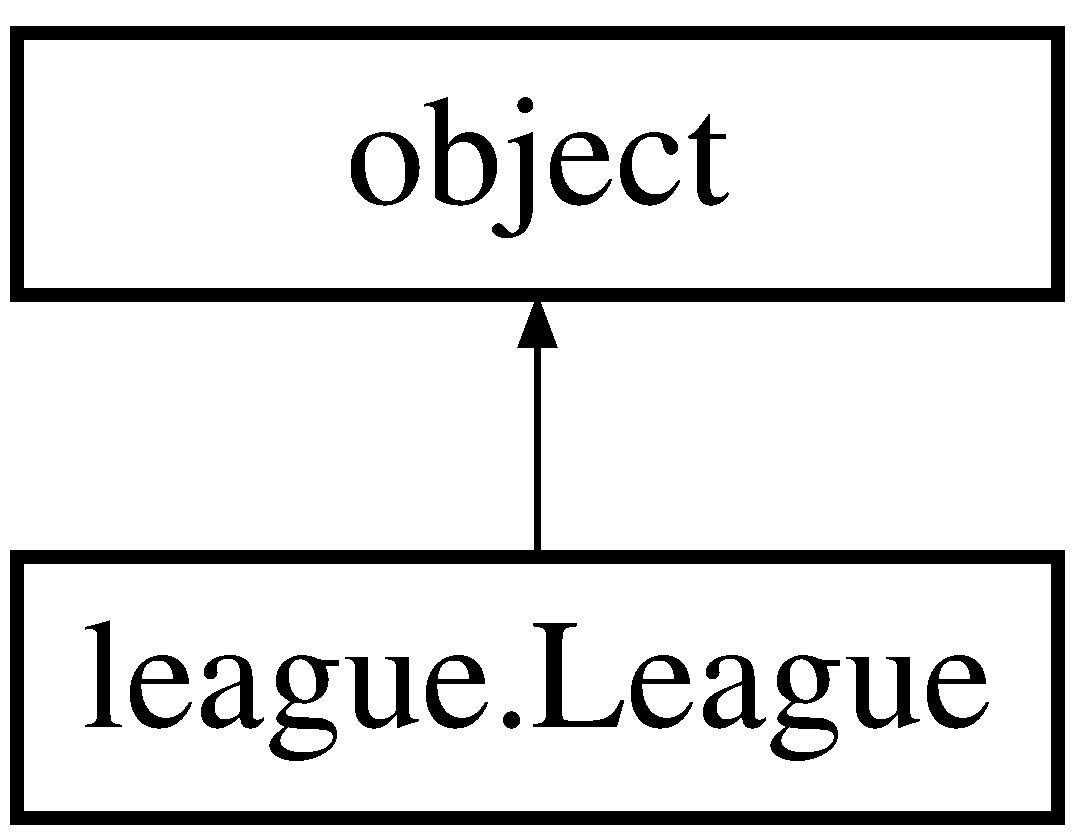
\includegraphics[height=2.000000cm]{classleague_1_1_league}
\end{center}
\end{figure}
\subsection*{Public Member Functions}
\begin{DoxyCompactItemize}
\item 
def \hyperlink{classleague_1_1_league_aad520cb765853c6173f9d8a9b9f92b65}{\+\_\+\+\_\+init\+\_\+\+\_\+} (self, league\+\_\+id)
\item 
def \hyperlink{classleague_1_1_league_acd15845f4b999982f4c454820a42d6c8}{get\+\_\+teams} (self)
\item 
def \hyperlink{classleague_1_1_league_a6a5d4954f2705402389247c274651f90}{get\+\_\+matches\+\_\+ids} (self)
\item 
def \hyperlink{classleague_1_1_league_aae35661491bbaf079af5b55ea161255b}{get\+\_\+lan\+\_\+matches\+\_\+ids} (self)
\item 
def \hyperlink{classleague_1_1_league_a8ee2c1b0200facaa7bdbcd975cd7034c}{show\+\_\+league\+\_\+info} (self)
\item 
def \hyperlink{classleague_1_1_league_a16576f2ee000b13680a0e3d85df22f57}{dump\+\_\+to\+\_\+file} (self, file\+\_\+name)
\item 
def \hyperlink{classleague_1_1_league_a1d8958ef5538a6fa0157d0c7c7f8f910}{get\+\_\+ti\+\_\+rosters} (self)
\item 
def \hyperlink{classleague_1_1_league_aa0799a0114eb19af4b8f40b505732636}{get\+\_\+rosters\+\_\+ids\+\_\+manual} ()
\item 
def {\bfseries get\+\_\+rosters\+\_\+ids\+\_\+manual} ()\hypertarget{classleague_1_1_league_aa0799a0114eb19af4b8f40b505732636}{}\label{classleague_1_1_league_aa0799a0114eb19af4b8f40b505732636}

\end{DoxyCompactItemize}
\subsection*{Public Attributes}
\begin{DoxyCompactItemize}
\item 
{\bfseries league\+\_\+id}\hypertarget{classleague_1_1_league_a0f90c5c4ca525bee48ddeb4e68024f93}{}\label{classleague_1_1_league_a0f90c5c4ca525bee48ddeb4e68024f93}

\item 
{\bfseries matches\+\_\+ids}\hypertarget{classleague_1_1_league_a4c36dc4e01574730afdb251f94d338a0}{}\label{classleague_1_1_league_a4c36dc4e01574730afdb251f94d338a0}

\item 
{\bfseries lan\+\_\+matches\+\_\+ids}\hypertarget{classleague_1_1_league_a237fd28b62a4cccbe2a7cf1e5896f4f8}{}\label{classleague_1_1_league_a237fd28b62a4cccbe2a7cf1e5896f4f8}

\item 
{\bfseries teams}\hypertarget{classleague_1_1_league_adfcb1b1a99da85c1f172724d4e4f1a2a}{}\label{classleague_1_1_league_adfcb1b1a99da85c1f172724d4e4f1a2a}

\item 
{\bfseries name}\hypertarget{classleague_1_1_league_a0b23879dba5aa1619953af45d3d9f95c}{}\label{classleague_1_1_league_a0b23879dba5aa1619953af45d3d9f95c}

\item 
{\bfseries lan\+\_\+matches}\hypertarget{classleague_1_1_league_a3c39a34ad0bdc4ec1054e92c80df37eb}{}\label{classleague_1_1_league_a3c39a34ad0bdc4ec1054e92c80df37eb}

\end{DoxyCompactItemize}


\subsection{Detailed Description}
\begin{DoxyVerb}Contains general info, lists of team's, matches's ids\end{DoxyVerb}
 

\subsection{Constructor \& Destructor Documentation}
\index{league\+::\+League@{league\+::\+League}!\+\_\+\+\_\+init\+\_\+\+\_\+@{\+\_\+\+\_\+init\+\_\+\+\_\+}}
\index{\+\_\+\+\_\+init\+\_\+\+\_\+@{\+\_\+\+\_\+init\+\_\+\+\_\+}!league\+::\+League@{league\+::\+League}}
\subsubsection[{\texorpdfstring{\+\_\+\+\_\+init\+\_\+\+\_\+(self, league\+\_\+id)}{\_\_init\_\_(self, league\_id)}}]{\setlength{\rightskip}{0pt plus 5cm}def league.\+League.\+\_\+\+\_\+init\+\_\+\+\_\+ (
\begin{DoxyParamCaption}
\item[{}]{self, }
\item[{}]{league\+\_\+id}
\end{DoxyParamCaption}
)}\hypertarget{classleague_1_1_league_aad520cb765853c6173f9d8a9b9f92b65}{}\label{classleague_1_1_league_aad520cb765853c6173f9d8a9b9f92b65}
\begin{DoxyVerb}Takes league_id
Creates object with name. To get matches etc use other functions.
\end{DoxyVerb}
 

\subsection{Member Function Documentation}
\index{league\+::\+League@{league\+::\+League}!dump\+\_\+to\+\_\+file@{dump\+\_\+to\+\_\+file}}
\index{dump\+\_\+to\+\_\+file@{dump\+\_\+to\+\_\+file}!league\+::\+League@{league\+::\+League}}
\subsubsection[{\texorpdfstring{dump\+\_\+to\+\_\+file(self, file\+\_\+name)}{dump\_to\_file(self, file\_name)}}]{\setlength{\rightskip}{0pt plus 5cm}def league.\+League.\+dump\+\_\+to\+\_\+file (
\begin{DoxyParamCaption}
\item[{}]{self, }
\item[{}]{file\+\_\+name}
\end{DoxyParamCaption}
)}\hypertarget{classleague_1_1_league_a16576f2ee000b13680a0e3d85df22f57}{}\label{classleague_1_1_league_a16576f2ee000b13680a0e3d85df22f57}
\begin{DoxyVerb}Parameters:
    file_name - str - variable from config, where to store data
\end{DoxyVerb}
 \index{league\+::\+League@{league\+::\+League}!get\+\_\+lan\+\_\+matches\+\_\+ids@{get\+\_\+lan\+\_\+matches\+\_\+ids}}
\index{get\+\_\+lan\+\_\+matches\+\_\+ids@{get\+\_\+lan\+\_\+matches\+\_\+ids}!league\+::\+League@{league\+::\+League}}
\subsubsection[{\texorpdfstring{get\+\_\+lan\+\_\+matches\+\_\+ids(self)}{get\_lan\_matches\_ids(self)}}]{\setlength{\rightskip}{0pt plus 5cm}def league.\+League.\+get\+\_\+lan\+\_\+matches\+\_\+ids (
\begin{DoxyParamCaption}
\item[{}]{self}
\end{DoxyParamCaption}
)}\hypertarget{classleague_1_1_league_aae35661491bbaf079af5b55ea161255b}{}\label{classleague_1_1_league_aae35661491bbaf079af5b55ea161255b}
\begin{DoxyVerb}won't work after august 2016, depends from month.
TODO: implement this for any tournament
\end{DoxyVerb}
 \index{league\+::\+League@{league\+::\+League}!get\+\_\+matches\+\_\+ids@{get\+\_\+matches\+\_\+ids}}
\index{get\+\_\+matches\+\_\+ids@{get\+\_\+matches\+\_\+ids}!league\+::\+League@{league\+::\+League}}
\subsubsection[{\texorpdfstring{get\+\_\+matches\+\_\+ids(self)}{get\_matches\_ids(self)}}]{\setlength{\rightskip}{0pt plus 5cm}def league.\+League.\+get\+\_\+matches\+\_\+ids (
\begin{DoxyParamCaption}
\item[{}]{self}
\end{DoxyParamCaption}
)}\hypertarget{classleague_1_1_league_a6a5d4954f2705402389247c274651f90}{}\label{classleague_1_1_league_a6a5d4954f2705402389247c274651f90}
\begin{DoxyVerb}Takes nothing.
Appends matches ids to self.matches_id from dotabuff
\end{DoxyVerb}
 \index{league\+::\+League@{league\+::\+League}!get\+\_\+rosters\+\_\+ids\+\_\+manual@{get\+\_\+rosters\+\_\+ids\+\_\+manual}}
\index{get\+\_\+rosters\+\_\+ids\+\_\+manual@{get\+\_\+rosters\+\_\+ids\+\_\+manual}!league\+::\+League@{league\+::\+League}}
\subsubsection[{\texorpdfstring{get\+\_\+rosters\+\_\+ids\+\_\+manual()}{get\_rosters\_ids\_manual()}}]{\setlength{\rightskip}{0pt plus 5cm}def league.\+League.\+get\+\_\+rosters\+\_\+ids\+\_\+manual (
\begin{DoxyParamCaption}
{}
\end{DoxyParamCaption}
)}\hypertarget{classleague_1_1_league_aa0799a0114eb19af4b8f40b505732636}{}\label{classleague_1_1_league_aa0799a0114eb19af4b8f40b505732636}
\begin{DoxyVerb}Gives opportunity to manually connect player name with account_id,
will be changed.
\end{DoxyVerb}
 \index{league\+::\+League@{league\+::\+League}!get\+\_\+teams@{get\+\_\+teams}}
\index{get\+\_\+teams@{get\+\_\+teams}!league\+::\+League@{league\+::\+League}}
\subsubsection[{\texorpdfstring{get\+\_\+teams(self)}{get\_teams(self)}}]{\setlength{\rightskip}{0pt plus 5cm}def league.\+League.\+get\+\_\+teams (
\begin{DoxyParamCaption}
\item[{}]{self}
\end{DoxyParamCaption}
)}\hypertarget{classleague_1_1_league_acd15845f4b999982f4c454820a42d6c8}{}\label{classleague_1_1_league_acd15845f4b999982f4c454820a42d6c8}
\begin{DoxyVerb}Takes self.
Adds Team class objects to league.
\end{DoxyVerb}
 \index{league\+::\+League@{league\+::\+League}!get\+\_\+ti\+\_\+rosters@{get\+\_\+ti\+\_\+rosters}}
\index{get\+\_\+ti\+\_\+rosters@{get\+\_\+ti\+\_\+rosters}!league\+::\+League@{league\+::\+League}}
\subsubsection[{\texorpdfstring{get\+\_\+ti\+\_\+rosters(self)}{get\_ti\_rosters(self)}}]{\setlength{\rightskip}{0pt plus 5cm}def league.\+League.\+get\+\_\+ti\+\_\+rosters (
\begin{DoxyParamCaption}
\item[{}]{self}
\end{DoxyParamCaption}
)}\hypertarget{classleague_1_1_league_a1d8958ef5538a6fa0157d0c7c7f8f910}{}\label{classleague_1_1_league_a1d8958ef5538a6fa0157d0c7c7f8f910}
\begin{DoxyVerb}NOTE: zai's and piliedie's names inserted in file manually.
Scrap official cite page dump to file teams rosters
\end{DoxyVerb}
 \index{league\+::\+League@{league\+::\+League}!show\+\_\+league\+\_\+info@{show\+\_\+league\+\_\+info}}
\index{show\+\_\+league\+\_\+info@{show\+\_\+league\+\_\+info}!league\+::\+League@{league\+::\+League}}
\subsubsection[{\texorpdfstring{show\+\_\+league\+\_\+info(self)}{show\_league\_info(self)}}]{\setlength{\rightskip}{0pt plus 5cm}def league.\+League.\+show\+\_\+league\+\_\+info (
\begin{DoxyParamCaption}
\item[{}]{self}
\end{DoxyParamCaption}
)}\hypertarget{classleague_1_1_league_a8ee2c1b0200facaa7bdbcd975cd7034c}{}\label{classleague_1_1_league_a8ee2c1b0200facaa7bdbcd975cd7034c}
\begin{DoxyVerb}Show name, id, amount of teams and games.
\end{DoxyVerb}
 

The documentation for this class was generated from the following file\+:\begin{DoxyCompactItemize}
\item 
deprecated/code/league.\+py\end{DoxyCompactItemize}

\hypertarget{classmatch_1_1_match}{}\section{match.\+Match Class Reference}
\label{classmatch_1_1_match}\index{match.\+Match@{match.\+Match}}
Inheritance diagram for match.\+Match\+:\begin{figure}[H]
\begin{center}
\leavevmode
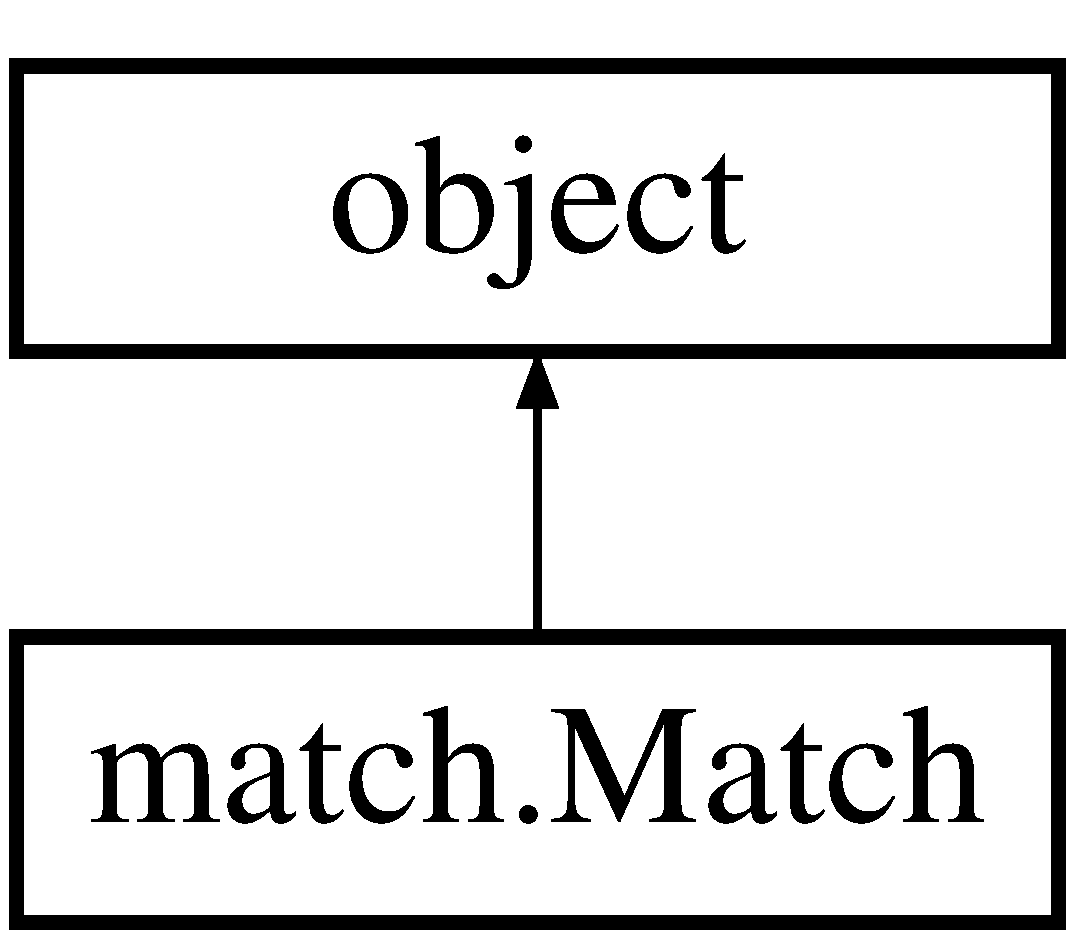
\includegraphics[height=2.000000cm]{classmatch_1_1_match}
\end{center}
\end{figure}
\subsection*{Public Member Functions}
\begin{DoxyCompactItemize}
\item 
def \hyperlink{classmatch_1_1_match_ab239e1d39b715e0f4a1e42ca04167baf}{\+\_\+\+\_\+init\+\_\+\+\_\+} (self, match\+\_\+id)
\item 
def \hyperlink{classmatch_1_1_match_a33c1e9af19bf97b7524d5e5c42d1091f}{compare\+\_\+features} (self)
\item 
def {\bfseries get\+\_\+teams\+\_\+info} (self)\hypertarget{classmatch_1_1_match_a7be5ae37fc2ddd3a049498845bbe02db}{}\label{classmatch_1_1_match_a7be5ae37fc2ddd3a049498845bbe02db}

\item 
def {\bfseries get\+\_\+teams\+\_\+features} (self)\hypertarget{classmatch_1_1_match_ab54e9ac8ac097926a253ecb60d1a8b46}{}\label{classmatch_1_1_match_ab54e9ac8ac097926a253ecb60d1a8b46}

\end{DoxyCompactItemize}
\subsection*{Public Attributes}
\begin{DoxyCompactItemize}
\item 
{\bfseries match\+\_\+id}\hypertarget{classmatch_1_1_match_ac7180a5643e6bb4655475ff7649976f1}{}\label{classmatch_1_1_match_ac7180a5643e6bb4655475ff7649976f1}

\item 
{\bfseries time}\hypertarget{classmatch_1_1_match_af1b6e0c4d181a9176b319f623d9a0b48}{}\label{classmatch_1_1_match_af1b6e0c4d181a9176b319f623d9a0b48}

\item 
{\bfseries result}\hypertarget{classmatch_1_1_match_a735edf1b04f1879827e6d81bf249fafc}{}\label{classmatch_1_1_match_a735edf1b04f1879827e6d81bf249fafc}

\item 
{\bfseries radiant}\hypertarget{classmatch_1_1_match_acb496c6dc781e9a3946a9ed02b2ec328}{}\label{classmatch_1_1_match_acb496c6dc781e9a3946a9ed02b2ec328}

\item 
{\bfseries dire}\hypertarget{classmatch_1_1_match_adc264c129d16d73ba0bb97dc5c4d4f2c}{}\label{classmatch_1_1_match_adc264c129d16d73ba0bb97dc5c4d4f2c}

\end{DoxyCompactItemize}


\subsection{Detailed Description}
\begin{DoxyVerb}docstring for Match\end{DoxyVerb}
 

\subsection{Constructor \& Destructor Documentation}
\index{match\+::\+Match@{match\+::\+Match}!\+\_\+\+\_\+init\+\_\+\+\_\+@{\+\_\+\+\_\+init\+\_\+\+\_\+}}
\index{\+\_\+\+\_\+init\+\_\+\+\_\+@{\+\_\+\+\_\+init\+\_\+\+\_\+}!match\+::\+Match@{match\+::\+Match}}
\subsubsection[{\texorpdfstring{\+\_\+\+\_\+init\+\_\+\+\_\+(self, match\+\_\+id)}{\_\_init\_\_(self, match\_id)}}]{\setlength{\rightskip}{0pt plus 5cm}def match.\+Match.\+\_\+\+\_\+init\+\_\+\+\_\+ (
\begin{DoxyParamCaption}
\item[{}]{self, }
\item[{}]{match\+\_\+id}
\end{DoxyParamCaption}
)}\hypertarget{classmatch_1_1_match_ab239e1d39b715e0f4a1e42ca04167baf}{}\label{classmatch_1_1_match_ab239e1d39b715e0f4a1e42ca04167baf}
\begin{DoxyVerb}Takes match_id
Creates Match object with:
    time - unix stamp
    result - true radiant won
    radiant, dire = Team()
\end{DoxyVerb}
 

\subsection{Member Function Documentation}
\index{match\+::\+Match@{match\+::\+Match}!compare\+\_\+features@{compare\+\_\+features}}
\index{compare\+\_\+features@{compare\+\_\+features}!match\+::\+Match@{match\+::\+Match}}
\subsubsection[{\texorpdfstring{compare\+\_\+features(self)}{compare\_features(self)}}]{\setlength{\rightskip}{0pt plus 5cm}def match.\+Match.\+compare\+\_\+features (
\begin{DoxyParamCaption}
\item[{}]{self}
\end{DoxyParamCaption}
)}\hypertarget{classmatch_1_1_match_a33c1e9af19bf97b7524d5e5c42d1091f}{}\label{classmatch_1_1_match_a33c1e9af19bf97b7524d5e5c42d1091f}
\begin{DoxyVerb}Will show you names of heroes and their features by sides
\end{DoxyVerb}
 

The documentation for this class was generated from the following file\+:\begin{DoxyCompactItemize}
\item 
deprecated/code/match.\+py\end{DoxyCompactItemize}

\hypertarget{classatod_1_1interfaces_1_1_member}{}\section{atod.\+interfaces.\+Member Class Reference}
\label{classatod_1_1interfaces_1_1_member}\index{atod.\+interfaces.\+Member@{atod.\+interfaces.\+Member}}
Inheritance diagram for atod.\+interfaces.\+Member\+:\begin{figure}[H]
\begin{center}
\leavevmode
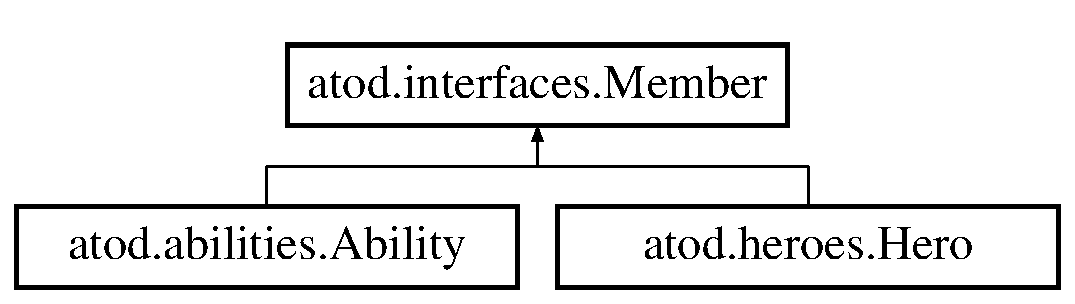
\includegraphics[height=2.000000cm]{classatod_1_1interfaces_1_1_member}
\end{center}
\end{figure}
\subsection*{Public Member Functions}
\begin{DoxyCompactItemize}
\item 
def \hyperlink{classatod_1_1interfaces_1_1_member_a7557bab11a65df8d39570804c9164d4f}{\+\_\+\+\_\+init\+\_\+\+\_\+} (self, id\+\_\+, name)
\item 
def \hyperlink{classatod_1_1interfaces_1_1_member_a00249f19c666de37fb983c717a994a49}{get\+\_\+description} (self)
\item 
def \hyperlink{classatod_1_1interfaces_1_1_member_a2b04b9db80fee2d437a8f989378d8dbd}{as\+\_\+dict} (self)
\end{DoxyCompactItemize}
\subsection*{Public Attributes}
\begin{DoxyCompactItemize}
\item 
{\bfseries id}\hypertarget{classatod_1_1interfaces_1_1_member_a14b6a3cf57d655d51c6495109ddde26b}{}\label{classatod_1_1interfaces_1_1_member_a14b6a3cf57d655d51c6495109ddde26b}

\item 
{\bfseries name}\hypertarget{classatod_1_1interfaces_1_1_member_acfbfe3c22092108af35c6961d7962e97}{}\label{classatod_1_1interfaces_1_1_member_acfbfe3c22092108af35c6961d7962e97}

\end{DoxyCompactItemize}
\subsection*{Static Public Attributes}
\begin{DoxyCompactItemize}
\item 
{\bfseries model} = None\hypertarget{classatod_1_1interfaces_1_1_member_ab2bc90f7f00167cfdc1e414eeb7b57d4}{}\label{classatod_1_1interfaces_1_1_member_ab2bc90f7f00167cfdc1e414eeb7b57d4}

\end{DoxyCompactItemize}


\subsection{Detailed Description}
\begin{DoxyVerb}The parent class for all the single elements.

    Attributes:
        model (sqlalchemy.ext.declarative.api.DeclarativeMeta): 
            SQlAlchemy based model which represents table in the db.
        id (int)  : unique identifier among other members.
        name (str): name.
\end{DoxyVerb}
 

\subsection{Constructor \& Destructor Documentation}
\index{atod\+::interfaces\+::\+Member@{atod\+::interfaces\+::\+Member}!\+\_\+\+\_\+init\+\_\+\+\_\+@{\+\_\+\+\_\+init\+\_\+\+\_\+}}
\index{\+\_\+\+\_\+init\+\_\+\+\_\+@{\+\_\+\+\_\+init\+\_\+\+\_\+}!atod\+::interfaces\+::\+Member@{atod\+::interfaces\+::\+Member}}
\subsubsection[{\texorpdfstring{\+\_\+\+\_\+init\+\_\+\+\_\+(self, id\+\_\+, name)}{\_\_init\_\_(self, id\_, name)}}]{\setlength{\rightskip}{0pt plus 5cm}def atod.\+interfaces.\+Member.\+\_\+\+\_\+init\+\_\+\+\_\+ (
\begin{DoxyParamCaption}
\item[{}]{self, }
\item[{}]{id\+\_\+, }
\item[{}]{name}
\end{DoxyParamCaption}
)}\hypertarget{classatod_1_1interfaces_1_1_member_a7557bab11a65df8d39570804c9164d4f}{}\label{classatod_1_1interfaces_1_1_member_a7557bab11a65df8d39570804c9164d4f}
\begin{DoxyVerb}Only initialise necessary attributes for any member. \end{DoxyVerb}
 

\subsection{Member Function Documentation}
\index{atod\+::interfaces\+::\+Member@{atod\+::interfaces\+::\+Member}!as\+\_\+dict@{as\+\_\+dict}}
\index{as\+\_\+dict@{as\+\_\+dict}!atod\+::interfaces\+::\+Member@{atod\+::interfaces\+::\+Member}}
\subsubsection[{\texorpdfstring{as\+\_\+dict(self)}{as\_dict(self)}}]{\setlength{\rightskip}{0pt plus 5cm}def atod.\+interfaces.\+Member.\+as\+\_\+dict (
\begin{DoxyParamCaption}
\item[{}]{self}
\end{DoxyParamCaption}
)}\hypertarget{classatod_1_1interfaces_1_1_member_a2b04b9db80fee2d437a8f989378d8dbd}{}\label{classatod_1_1interfaces_1_1_member_a2b04b9db80fee2d437a8f989378d8dbd}
\begin{DoxyVerb}Returns representation of this object as a dictionary.\end{DoxyVerb}
 \index{atod\+::interfaces\+::\+Member@{atod\+::interfaces\+::\+Member}!get\+\_\+description@{get\+\_\+description}}
\index{get\+\_\+description@{get\+\_\+description}!atod\+::interfaces\+::\+Member@{atod\+::interfaces\+::\+Member}}
\subsubsection[{\texorpdfstring{get\+\_\+description(self)}{get\_description(self)}}]{\setlength{\rightskip}{0pt plus 5cm}def atod.\+interfaces.\+Member.\+get\+\_\+description (
\begin{DoxyParamCaption}
\item[{}]{self}
\end{DoxyParamCaption}
)}\hypertarget{classatod_1_1interfaces_1_1_member_a00249f19c666de37fb983c717a994a49}{}\label{classatod_1_1interfaces_1_1_member_a00249f19c666de37fb983c717a994a49}
\begin{DoxyVerb}Returns a object as a pd.Series. 

    Returns:
vector (pandas.Series): representation of the object\end{DoxyVerb}
 

The documentation for this class was generated from the following file\+:\begin{DoxyCompactItemize}
\item 
atod/interfaces.\+py\end{DoxyCompactItemize}

\hypertarget{classatod_1_1tests_1_1test__hero__model_1_1_my_test_case}{}\section{atod.\+tests.\+test\+\_\+hero\+\_\+model.\+My\+Test\+Case Class Reference}
\label{classatod_1_1tests_1_1test__hero__model_1_1_my_test_case}\index{atod.\+tests.\+test\+\_\+hero\+\_\+model.\+My\+Test\+Case@{atod.\+tests.\+test\+\_\+hero\+\_\+model.\+My\+Test\+Case}}
Inheritance diagram for atod.\+tests.\+test\+\_\+hero\+\_\+model.\+My\+Test\+Case\+:\begin{figure}[H]
\begin{center}
\leavevmode
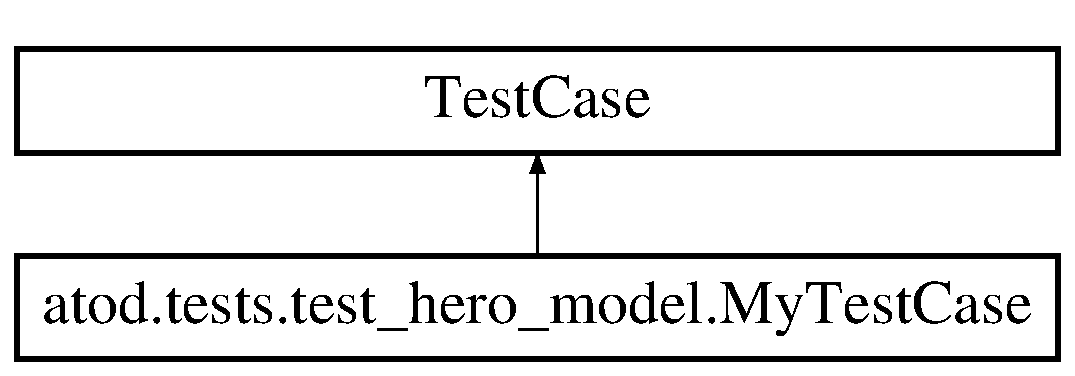
\includegraphics[height=2.000000cm]{classatod_1_1tests_1_1test__hero__model_1_1_my_test_case}
\end{center}
\end{figure}
\subsection*{Public Member Functions}
\begin{DoxyCompactItemize}
\item 
def {\bfseries test\+\_\+attributes} (self)\hypertarget{classatod_1_1tests_1_1test__hero__model_1_1_my_test_case_aa1c40260186074876e6b1879be830448}{}\label{classatod_1_1tests_1_1test__hero__model_1_1_my_test_case_aa1c40260186074876e6b1879be830448}

\end{DoxyCompactItemize}


The documentation for this class was generated from the following file\+:\begin{DoxyCompactItemize}
\item 
atod/tests/test\+\_\+hero\+\_\+model.\+py\end{DoxyCompactItemize}

\hypertarget{classpick_1_1_pick}{}\section{pick.\+Pick Class Reference}
\label{classpick_1_1_pick}\index{pick.\+Pick@{pick.\+Pick}}
Inheritance diagram for pick.\+Pick\+:\begin{figure}[H]
\begin{center}
\leavevmode
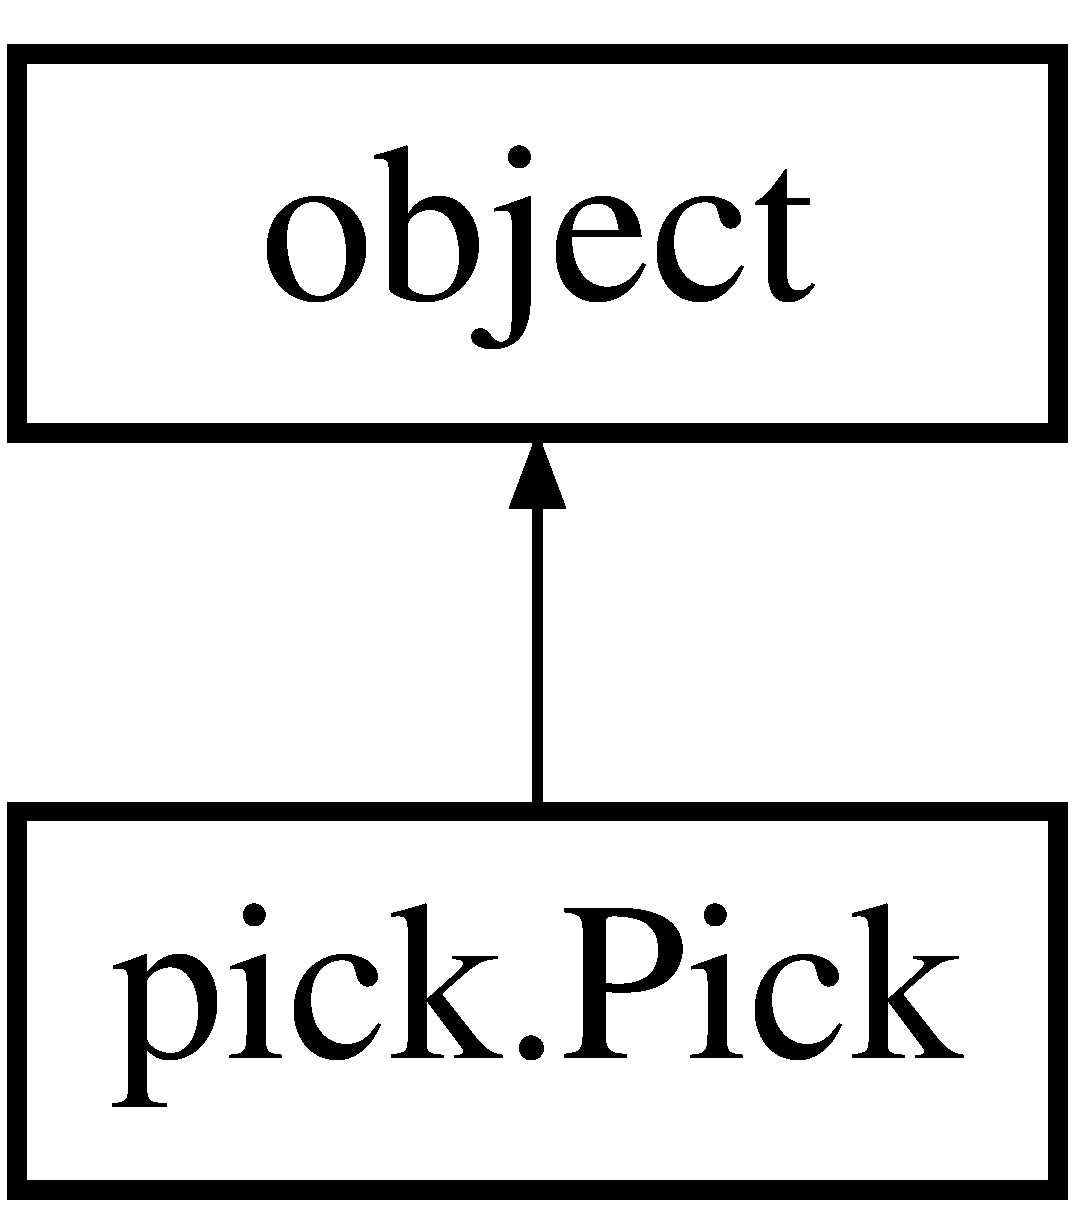
\includegraphics[height=2.000000cm]{classpick_1_1_pick}
\end{center}
\end{figure}
\subsection*{Public Member Functions}
\begin{DoxyCompactItemize}
\item 
def \hyperlink{classpick_1_1_pick_ab5dfdc4884d79ca0d9c8bdc9087d13e0}{\+\_\+\+\_\+init\+\_\+\+\_\+} (self, arg)
\item 
def {\bfseries add\+\_\+hero} (self, hero)\hypertarget{classpick_1_1_pick_a3924e68fa65169363b187cf9da662833}{}\label{classpick_1_1_pick_a3924e68fa65169363b187cf9da662833}

\item 
def \hyperlink{classpick_1_1_pick_aca17179c68e00a8ff3f6fff44a78c273}{show\+\_\+heroes} (self)
\item 
def \hyperlink{classpick_1_1_pick_aed47b3e5a260b2620c0f6b7a28f81680}{get\+\_\+features\+\_\+sum} (self)
\item 
def {\bfseries show\+\_\+features} (self)\hypertarget{classpick_1_1_pick_ade057b1384dc1df25fc68a5fe2e8b2f8}{}\label{classpick_1_1_pick_ade057b1384dc1df25fc68a5fe2e8b2f8}

\end{DoxyCompactItemize}
\subsection*{Public Attributes}
\begin{DoxyCompactItemize}
\item 
{\bfseries heroes}\hypertarget{classpick_1_1_pick_aebc6188a9c8bc4852a747d073af68a4a}{}\label{classpick_1_1_pick_aebc6188a9c8bc4852a747d073af68a4a}

\item 
{\bfseries features}\hypertarget{classpick_1_1_pick_ad8ca33d7e3d1b4ea525653254f1232b8}{}\label{classpick_1_1_pick_ad8ca33d7e3d1b4ea525653254f1232b8}

\end{DoxyCompactItemize}


\subsection{Detailed Description}
\begin{DoxyVerb}Contain list of heroes and sum of their features\end{DoxyVerb}
 

\subsection{Constructor \& Destructor Documentation}
\index{pick\+::\+Pick@{pick\+::\+Pick}!\+\_\+\+\_\+init\+\_\+\+\_\+@{\+\_\+\+\_\+init\+\_\+\+\_\+}}
\index{\+\_\+\+\_\+init\+\_\+\+\_\+@{\+\_\+\+\_\+init\+\_\+\+\_\+}!pick\+::\+Pick@{pick\+::\+Pick}}
\subsubsection[{\texorpdfstring{\+\_\+\+\_\+init\+\_\+\+\_\+(self, arg)}{\_\_init\_\_(self, arg)}}]{\setlength{\rightskip}{0pt plus 5cm}def pick.\+Pick.\+\_\+\+\_\+init\+\_\+\+\_\+ (
\begin{DoxyParamCaption}
\item[{}]{self, }
\item[{}]{arg}
\end{DoxyParamCaption}
)}\hypertarget{classpick_1_1_pick_ab5dfdc4884d79ca0d9c8bdc9087d13e0}{}\label{classpick_1_1_pick_ab5dfdc4884d79ca0d9c8bdc9087d13e0}
\begin{DoxyVerb}Takes list of id (can be empty)
\end{DoxyVerb}
 

\subsection{Member Function Documentation}
\index{pick\+::\+Pick@{pick\+::\+Pick}!get\+\_\+features\+\_\+sum@{get\+\_\+features\+\_\+sum}}
\index{get\+\_\+features\+\_\+sum@{get\+\_\+features\+\_\+sum}!pick\+::\+Pick@{pick\+::\+Pick}}
\subsubsection[{\texorpdfstring{get\+\_\+features\+\_\+sum(self)}{get\_features\_sum(self)}}]{\setlength{\rightskip}{0pt plus 5cm}def pick.\+Pick.\+get\+\_\+features\+\_\+sum (
\begin{DoxyParamCaption}
\item[{}]{self}
\end{DoxyParamCaption}
)}\hypertarget{classpick_1_1_pick_aed47b3e5a260b2620c0f6b7a28f81680}{}\label{classpick_1_1_pick_aed47b3e5a260b2620c0f6b7a28f81680}
\begin{DoxyVerb}Takes name of json file with features
Writes sum of heroes features to self.features
Returns nothing
\end{DoxyVerb}
 \index{pick\+::\+Pick@{pick\+::\+Pick}!show\+\_\+heroes@{show\+\_\+heroes}}
\index{show\+\_\+heroes@{show\+\_\+heroes}!pick\+::\+Pick@{pick\+::\+Pick}}
\subsubsection[{\texorpdfstring{show\+\_\+heroes(self)}{show\_heroes(self)}}]{\setlength{\rightskip}{0pt plus 5cm}def pick.\+Pick.\+show\+\_\+heroes (
\begin{DoxyParamCaption}
\item[{}]{self}
\end{DoxyParamCaption}
)}\hypertarget{classpick_1_1_pick_aca17179c68e00a8ff3f6fff44a78c273}{}\label{classpick_1_1_pick_aca17179c68e00a8ff3f6fff44a78c273}
\begin{DoxyVerb}Print names of heroes\end{DoxyVerb}
 

The documentation for this class was generated from the following file\+:\begin{DoxyCompactItemize}
\item 
deprecated/code/pick.\+py\end{DoxyCompactItemize}

\hypertarget{classplayer_1_1_player}{}\section{player.\+Player Class Reference}
\label{classplayer_1_1_player}\index{player.\+Player@{player.\+Player}}
Inheritance diagram for player.\+Player\+:\begin{figure}[H]
\begin{center}
\leavevmode
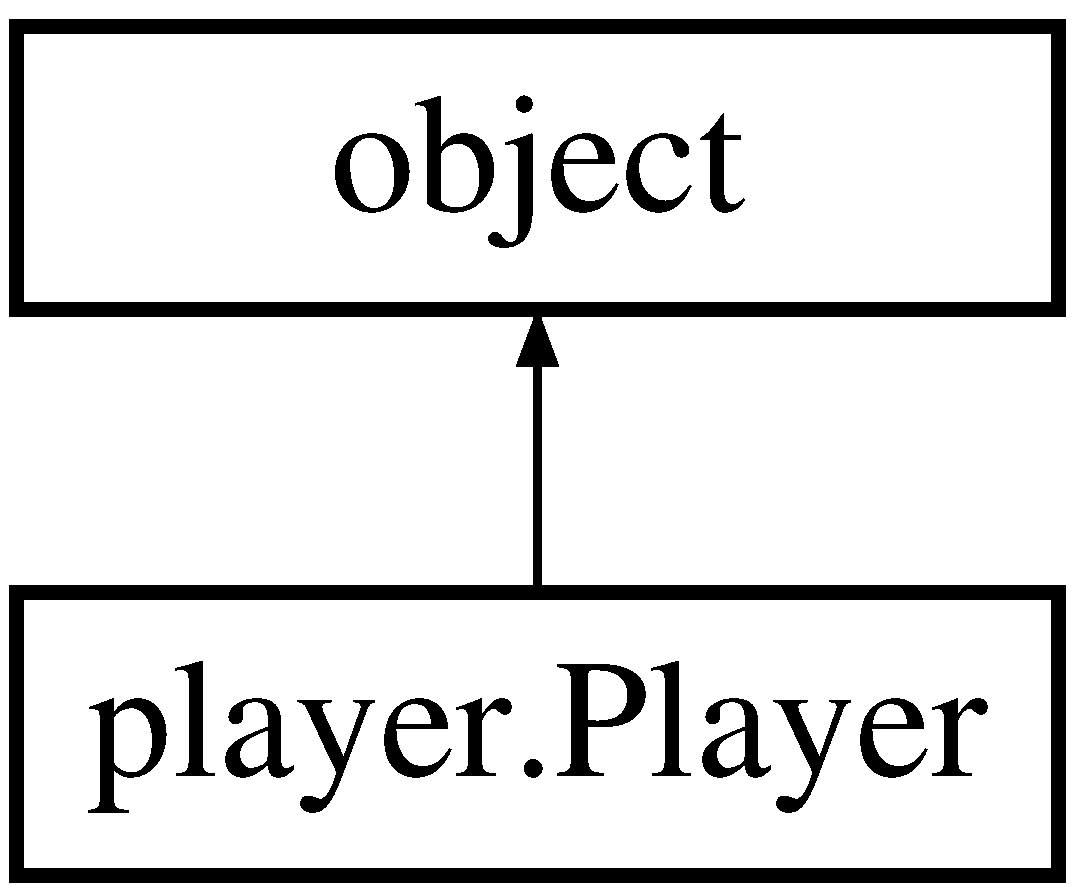
\includegraphics[height=2.000000cm]{classplayer_1_1_player}
\end{center}
\end{figure}
\subsection*{Public Member Functions}
\begin{DoxyCompactItemize}
\item 
def {\bfseries \+\_\+\+\_\+init\+\_\+\+\_\+} (self, player\+\_\+dict, features\+\_\+dict)\hypertarget{classplayer_1_1_player_a2415ed4a4b8bf46fa0ac707e54234f71}{}\label{classplayer_1_1_player_a2415ed4a4b8bf46fa0ac707e54234f71}

\item 
def \hyperlink{classplayer_1_1_player_a761d25515133bdc491119aa2e8630ecc}{show\+\_\+features} (self)
\item 
def \hyperlink{classplayer_1_1_player_a3593ddb31b6826c30ce34a1b648609d8}{set\+\_\+role} (self, acc\+\_\+id\+\_\+to\+\_\+role)
\end{DoxyCompactItemize}
\subsection*{Public Attributes}
\begin{DoxyCompactItemize}
\item 
{\bfseries account\+\_\+id}\hypertarget{classplayer_1_1_player_a0ab00a27d2cacb26530bcba6491a2ceb}{}\label{classplayer_1_1_player_a0ab00a27d2cacb26530bcba6491a2ceb}

\item 
{\bfseries hero\+\_\+id}\hypertarget{classplayer_1_1_player_a51f32411dbe933f4c542291294cfae34}{}\label{classplayer_1_1_player_a51f32411dbe933f4c542291294cfae34}

\item 
{\bfseries role}\hypertarget{classplayer_1_1_player_a8bb4462ad80ce41651e9684a7718f598}{}\label{classplayer_1_1_player_a8bb4462ad80ce41651e9684a7718f598}

\item 
{\bfseries features}\hypertarget{classplayer_1_1_player_a439d29a6102a63d9dab0db52616c8c1b}{}\label{classplayer_1_1_player_a439d29a6102a63d9dab0db52616c8c1b}

\end{DoxyCompactItemize}


\subsection{Detailed Description}
\begin{DoxyVerb}docstring for Player\end{DoxyVerb}
 

\subsection{Member Function Documentation}
\index{player\+::\+Player@{player\+::\+Player}!set\+\_\+role@{set\+\_\+role}}
\index{set\+\_\+role@{set\+\_\+role}!player\+::\+Player@{player\+::\+Player}}
\subsubsection[{\texorpdfstring{set\+\_\+role(self, acc\+\_\+id\+\_\+to\+\_\+role)}{set\_role(self, acc\_id\_to\_role)}}]{\setlength{\rightskip}{0pt plus 5cm}def player.\+Player.\+set\+\_\+role (
\begin{DoxyParamCaption}
\item[{}]{self, }
\item[{}]{acc\+\_\+id\+\_\+to\+\_\+role}
\end{DoxyParamCaption}
)}\hypertarget{classplayer_1_1_player_a3593ddb31b6826c30ce34a1b648609d8}{}\label{classplayer_1_1_player_a3593ddb31b6826c30ce34a1b648609d8}
\begin{DoxyVerb}will print account_id if hero there is no such hero in 
acc_id_to role sictionary
\end{DoxyVerb}
 \index{player\+::\+Player@{player\+::\+Player}!show\+\_\+features@{show\+\_\+features}}
\index{show\+\_\+features@{show\+\_\+features}!player\+::\+Player@{player\+::\+Player}}
\subsubsection[{\texorpdfstring{show\+\_\+features(self)}{show\_features(self)}}]{\setlength{\rightskip}{0pt plus 5cm}def player.\+Player.\+show\+\_\+features (
\begin{DoxyParamCaption}
\item[{}]{self}
\end{DoxyParamCaption}
)}\hypertarget{classplayer_1_1_player_a761d25515133bdc491119aa2e8630ecc}{}\label{classplayer_1_1_player_a761d25515133bdc491119aa2e8630ecc}
\begin{DoxyVerb}prints hero name and list of features
\end{DoxyVerb}
 

The documentation for this class was generated from the following file\+:\begin{DoxyCompactItemize}
\item 
deprecated/code/player.\+py\end{DoxyCompactItemize}

\hypertarget{classabilities__old_1_1_singleton}{}\section{abilities\+\_\+old.\+Singleton Class Reference}
\label{classabilities__old_1_1_singleton}\index{abilities\+\_\+old.\+Singleton@{abilities\+\_\+old.\+Singleton}}
Inheritance diagram for abilities\+\_\+old.\+Singleton\+:\begin{figure}[H]
\begin{center}
\leavevmode
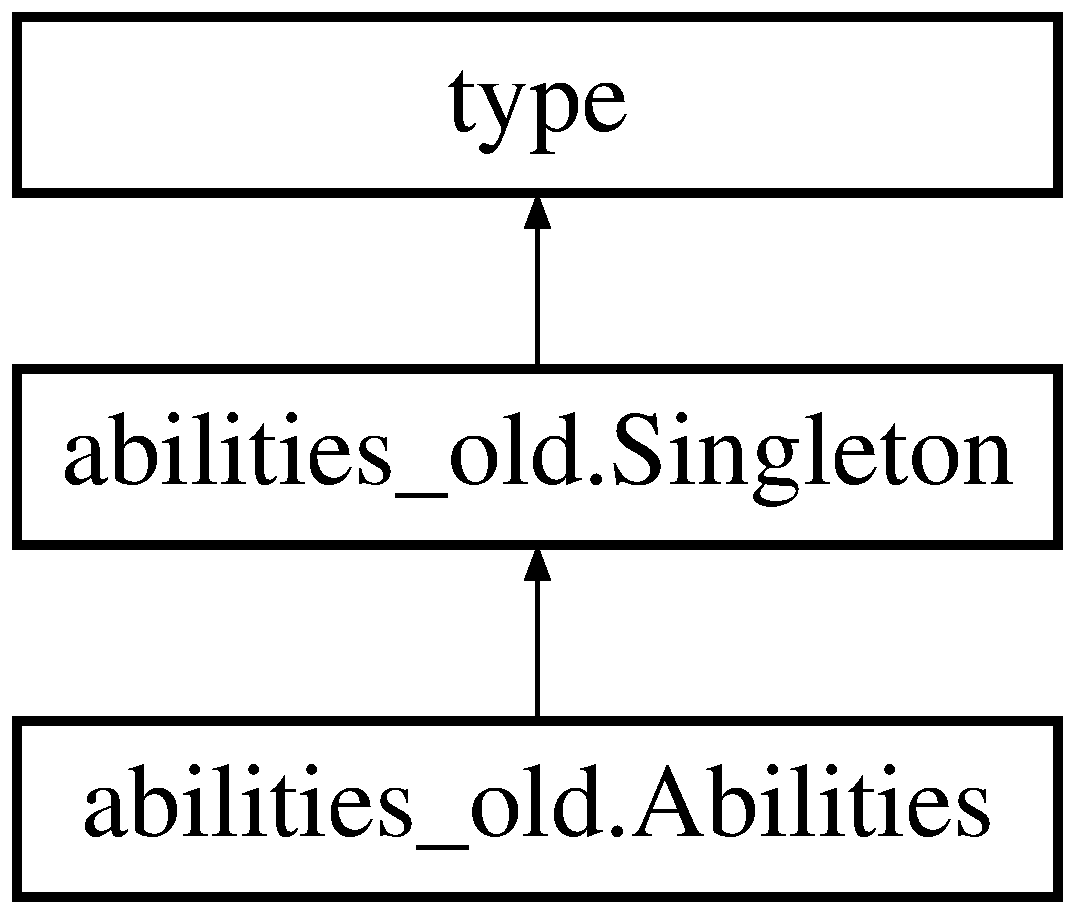
\includegraphics[height=3.000000cm]{classabilities__old_1_1_singleton}
\end{center}
\end{figure}
\subsection*{Public Member Functions}
\begin{DoxyCompactItemize}
\item 
def {\bfseries \+\_\+\+\_\+call\+\_\+\+\_\+} (cls, args, kwargs)\hypertarget{classabilities__old_1_1_singleton_a4ddd79ab5ff5c498eba711693507d60b}{}\label{classabilities__old_1_1_singleton_a4ddd79ab5ff5c498eba711693507d60b}

\end{DoxyCompactItemize}


The documentation for this class was generated from the following file\+:\begin{DoxyCompactItemize}
\item 
deprecated/abilities\+\_\+old.\+py\end{DoxyCompactItemize}

\hypertarget{classteam_1_1_team}{}\section{team.\+Team Class Reference}
\label{classteam_1_1_team}\index{team.\+Team@{team.\+Team}}
Inheritance diagram for team.\+Team\+:\begin{figure}[H]
\begin{center}
\leavevmode
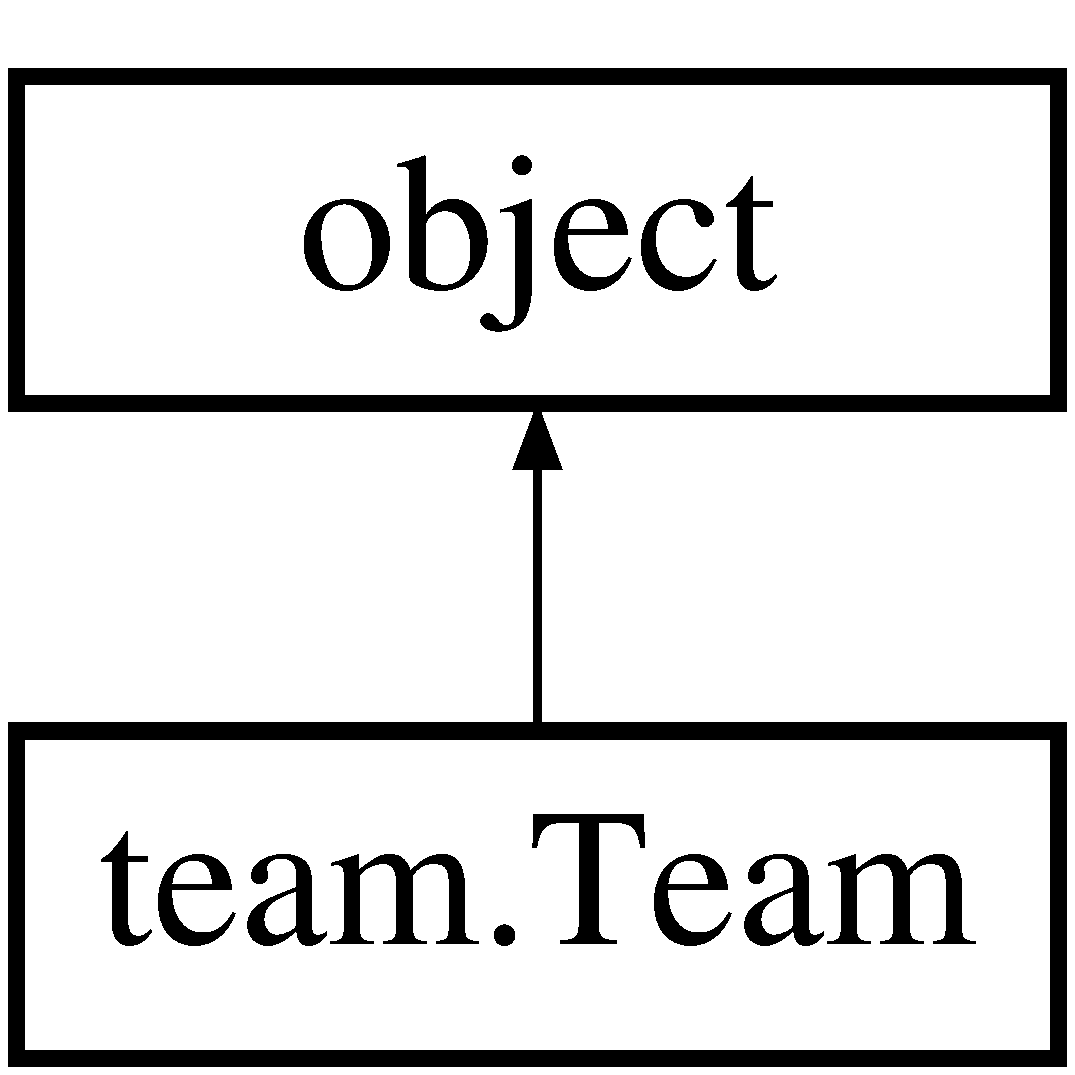
\includegraphics[height=2.000000cm]{classteam_1_1_team}
\end{center}
\end{figure}
\subsection*{Public Member Functions}
\begin{DoxyCompactItemize}
\item 
def \hyperlink{classteam_1_1_team_af834639269e343fbacc3d99e815e032f}{\+\_\+\+\_\+init\+\_\+\+\_\+} (self, team\+\_\+dict)
\item 
def \hyperlink{classteam_1_1_team_aab666e3bf7955f682b49898f251b81e4}{as\+\_\+dict} (self)
\item 
def \hyperlink{classteam_1_1_team_a74cff94194e1af6154dfdd7215423e24}{show\+\_\+features} (self)
\item 
def \hyperlink{classteam_1_1_team_af64128503d74e76b9ba76598faae292c}{sort\+\_\+players\+\_\+by\+\_\+role} (self)
\item 
def {\bfseries return\+\_\+info\+\_\+to\+\_\+db} (self)\hypertarget{classteam_1_1_team_a49df92cb20425e8e128c895c92d85662}{}\label{classteam_1_1_team_a49df92cb20425e8e128c895c92d85662}

\item 
def {\bfseries get\+\_\+features\+\_\+sum} (self)\hypertarget{classteam_1_1_team_aa8986fa35041bc005111a580b80aff8a}{}\label{classteam_1_1_team_aa8986fa35041bc005111a580b80aff8a}

\end{DoxyCompactItemize}
\subsection*{Public Attributes}
\begin{DoxyCompactItemize}
\item 
{\bfseries name}\hypertarget{classteam_1_1_team_a8288175f1c0568b3b7e8c26c24987568}{}\label{classteam_1_1_team_a8288175f1c0568b3b7e8c26c24987568}

\item 
{\bfseries team\+\_\+id}\hypertarget{classteam_1_1_team_a68db6b193a7fe2ad9325d333c89c34b5}{}\label{classteam_1_1_team_a68db6b193a7fe2ad9325d333c89c34b5}

\item 
{\bfseries heroes\+\_\+ids}\hypertarget{classteam_1_1_team_a3af8e3b765bd0c9cc64752ae3102dbf3}{}\label{classteam_1_1_team_a3af8e3b765bd0c9cc64752ae3102dbf3}

\item 
{\bfseries players}\hypertarget{classteam_1_1_team_a2596bc50a439e83e9827166468f0bbdc}{}\label{classteam_1_1_team_a2596bc50a439e83e9827166468f0bbdc}

\item 
{\bfseries features}\hypertarget{classteam_1_1_team_a651910f0947a1f3b680d66389294b8d3}{}\label{classteam_1_1_team_a651910f0947a1f3b680d66389294b8d3}

\end{DoxyCompactItemize}


\subsection{Detailed Description}
\begin{DoxyVerb}docstring for Team\end{DoxyVerb}
 

\subsection{Constructor \& Destructor Documentation}
\index{team\+::\+Team@{team\+::\+Team}!\+\_\+\+\_\+init\+\_\+\+\_\+@{\+\_\+\+\_\+init\+\_\+\+\_\+}}
\index{\+\_\+\+\_\+init\+\_\+\+\_\+@{\+\_\+\+\_\+init\+\_\+\+\_\+}!team\+::\+Team@{team\+::\+Team}}
\subsubsection[{\texorpdfstring{\+\_\+\+\_\+init\+\_\+\+\_\+(self, team\+\_\+dict)}{\_\_init\_\_(self, team\_dict)}}]{\setlength{\rightskip}{0pt plus 5cm}def team.\+Team.\+\_\+\+\_\+init\+\_\+\+\_\+ (
\begin{DoxyParamCaption}
\item[{}]{self, }
\item[{}]{team\+\_\+dict}
\end{DoxyParamCaption}
)}\hypertarget{classteam_1_1_team_af834639269e343fbacc3d99e815e032f}{}\label{classteam_1_1_team_af834639269e343fbacc3d99e815e032f}
\begin{DoxyVerb}Takes dictionary with 'name', 'team_id', 'heroes_id'
\end{DoxyVerb}
 

\subsection{Member Function Documentation}
\index{team\+::\+Team@{team\+::\+Team}!as\+\_\+dict@{as\+\_\+dict}}
\index{as\+\_\+dict@{as\+\_\+dict}!team\+::\+Team@{team\+::\+Team}}
\subsubsection[{\texorpdfstring{as\+\_\+dict(self)}{as\_dict(self)}}]{\setlength{\rightskip}{0pt plus 5cm}def team.\+Team.\+as\+\_\+dict (
\begin{DoxyParamCaption}
\item[{}]{self}
\end{DoxyParamCaption}
)}\hypertarget{classteam_1_1_team_aab666e3bf7955f682b49898f251b81e4}{}\label{classteam_1_1_team_aab666e3bf7955f682b49898f251b81e4}
\begin{DoxyVerb}I don't remember why i need this\end{DoxyVerb}
 \index{team\+::\+Team@{team\+::\+Team}!show\+\_\+features@{show\+\_\+features}}
\index{show\+\_\+features@{show\+\_\+features}!team\+::\+Team@{team\+::\+Team}}
\subsubsection[{\texorpdfstring{show\+\_\+features(self)}{show\_features(self)}}]{\setlength{\rightskip}{0pt plus 5cm}def team.\+Team.\+show\+\_\+features (
\begin{DoxyParamCaption}
\item[{}]{self}
\end{DoxyParamCaption}
)}\hypertarget{classteam_1_1_team_a74cff94194e1af6154dfdd7215423e24}{}\label{classteam_1_1_team_a74cff94194e1af6154dfdd7215423e24}
\begin{DoxyVerb}Shows every player features
\end{DoxyVerb}
 \index{team\+::\+Team@{team\+::\+Team}!sort\+\_\+players\+\_\+by\+\_\+role@{sort\+\_\+players\+\_\+by\+\_\+role}}
\index{sort\+\_\+players\+\_\+by\+\_\+role@{sort\+\_\+players\+\_\+by\+\_\+role}!team\+::\+Team@{team\+::\+Team}}
\subsubsection[{\texorpdfstring{sort\+\_\+players\+\_\+by\+\_\+role(self)}{sort\_players\_by\_role(self)}}]{\setlength{\rightskip}{0pt plus 5cm}def team.\+Team.\+sort\+\_\+players\+\_\+by\+\_\+role (
\begin{DoxyParamCaption}
\item[{}]{self}
\end{DoxyParamCaption}
)}\hypertarget{classteam_1_1_team_af64128503d74e76b9ba76598faae292c}{}\label{classteam_1_1_team_af64128503d74e76b9ba76598faae292c}
\begin{DoxyVerb}Sorts self.players by role from 1 to 5
\end{DoxyVerb}
 

The documentation for this class was generated from the following file\+:\begin{DoxyCompactItemize}
\item 
deprecated/code/team.\+py\end{DoxyCompactItemize}

\hypertarget{classtest__abilities_1_1_test_abilities}{}\section{test\+\_\+abilities.\+Test\+Abilities Class Reference}
\label{classtest__abilities_1_1_test_abilities}\index{test\+\_\+abilities.\+Test\+Abilities@{test\+\_\+abilities.\+Test\+Abilities}}
Inheritance diagram for test\+\_\+abilities.\+Test\+Abilities\+:\begin{figure}[H]
\begin{center}
\leavevmode
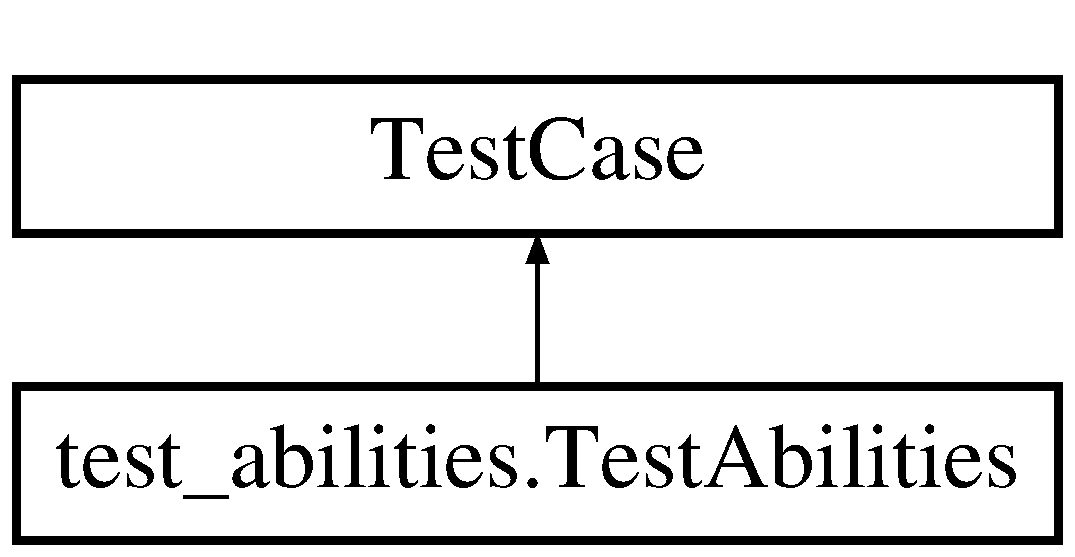
\includegraphics[height=2.000000cm]{classtest__abilities_1_1_test_abilities}
\end{center}
\end{figure}
\subsection*{Public Member Functions}
\begin{DoxyCompactItemize}
\item 
def \hyperlink{classtest__abilities_1_1_test_abilities_afbdc21fa88b58751a5373b815800f786}{test\+\_\+effects\+\_\+extraction} (self)
\item 
def \hyperlink{classtest__abilities_1_1_test_abilities_a1452657ffce85ad97f3aeec1e8dab911}{test\+\_\+frame\+\_\+shape} (self)
\end{DoxyCompactItemize}


\subsection{Member Function Documentation}
\index{test\+\_\+abilities\+::\+Test\+Abilities@{test\+\_\+abilities\+::\+Test\+Abilities}!test\+\_\+effects\+\_\+extraction@{test\+\_\+effects\+\_\+extraction}}
\index{test\+\_\+effects\+\_\+extraction@{test\+\_\+effects\+\_\+extraction}!test\+\_\+abilities\+::\+Test\+Abilities@{test\+\_\+abilities\+::\+Test\+Abilities}}
\subsubsection[{\texorpdfstring{test\+\_\+effects\+\_\+extraction(self)}{test\_effects\_extraction(self)}}]{\setlength{\rightskip}{0pt plus 5cm}def test\+\_\+abilities.\+Test\+Abilities.\+test\+\_\+effects\+\_\+extraction (
\begin{DoxyParamCaption}
\item[{}]{self}
\end{DoxyParamCaption}
)}\hypertarget{classtest__abilities_1_1_test_abilities_afbdc21fa88b58751a5373b815800f786}{}\label{classtest__abilities_1_1_test_abilities_afbdc21fa88b58751a5373b815800f786}
\begin{DoxyVerb}Tests effects property.\end{DoxyVerb}
 \index{test\+\_\+abilities\+::\+Test\+Abilities@{test\+\_\+abilities\+::\+Test\+Abilities}!test\+\_\+frame\+\_\+shape@{test\+\_\+frame\+\_\+shape}}
\index{test\+\_\+frame\+\_\+shape@{test\+\_\+frame\+\_\+shape}!test\+\_\+abilities\+::\+Test\+Abilities@{test\+\_\+abilities\+::\+Test\+Abilities}}
\subsubsection[{\texorpdfstring{test\+\_\+frame\+\_\+shape(self)}{test\_frame\_shape(self)}}]{\setlength{\rightskip}{0pt plus 5cm}def test\+\_\+abilities.\+Test\+Abilities.\+test\+\_\+frame\+\_\+shape (
\begin{DoxyParamCaption}
\item[{}]{self}
\end{DoxyParamCaption}
)}\hypertarget{classtest__abilities_1_1_test_abilities_a1452657ffce85ad97f3aeec1e8dab911}{}\label{classtest__abilities_1_1_test_abilities_a1452657ffce85ad97f3aeec1e8dab911}
\begin{DoxyVerb}Very long test, since whole DataFrame is created.\end{DoxyVerb}
 

The documentation for this class was generated from the following file\+:\begin{DoxyCompactItemize}
\item 
deprecated/test\+\_\+abilities.\+py\end{DoxyCompactItemize}

\hypertarget{classatod_1_1tests_1_1test__cleaninng__abilities_1_1_test_cleaning_abilities}{}\section{atod.\+tests.\+test\+\_\+cleaninng\+\_\+abilities.\+Test\+Cleaning\+Abilities Class Reference}
\label{classatod_1_1tests_1_1test__cleaninng__abilities_1_1_test_cleaning_abilities}\index{atod.\+tests.\+test\+\_\+cleaninng\+\_\+abilities.\+Test\+Cleaning\+Abilities@{atod.\+tests.\+test\+\_\+cleaninng\+\_\+abilities.\+Test\+Cleaning\+Abilities}}
Inheritance diagram for atod.\+tests.\+test\+\_\+cleaninng\+\_\+abilities.\+Test\+Cleaning\+Abilities\+:\begin{figure}[H]
\begin{center}
\leavevmode
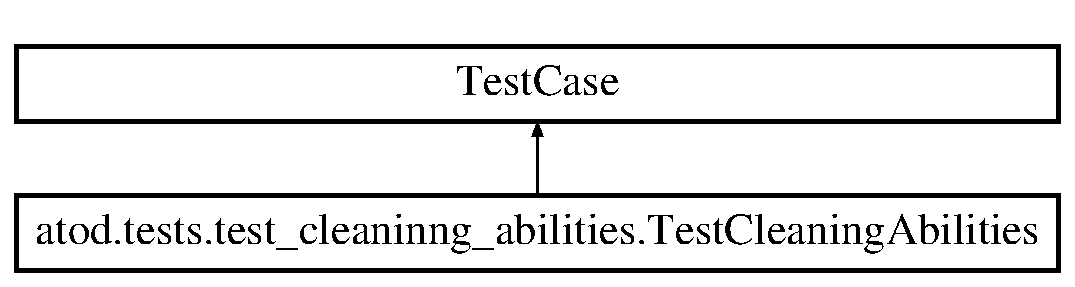
\includegraphics[height=2.000000cm]{classatod_1_1tests_1_1test__cleaninng__abilities_1_1_test_cleaning_abilities}
\end{center}
\end{figure}
\subsection*{Public Member Functions}
\begin{DoxyCompactItemize}
\item 
def {\bfseries set\+Up} (self)\hypertarget{classatod_1_1tests_1_1test__cleaninng__abilities_1_1_test_cleaning_abilities_aecfd3bb389a487384661abb9b0f5ef78}{}\label{classatod_1_1tests_1_1test__cleaninng__abilities_1_1_test_cleaning_abilities_aecfd3bb389a487384661abb9b0f5ef78}

\item 
def {\bfseries test\+\_\+average\+\_\+properties} (self)\hypertarget{classatod_1_1tests_1_1test__cleaninng__abilities_1_1_test_cleaning_abilities_a93403e9282cdc7dced771bf371d54341}{}\label{classatod_1_1tests_1_1test__cleaninng__abilities_1_1_test_cleaning_abilities_a93403e9282cdc7dced771bf371d54341}

\item 
def {\bfseries test\+\_\+tooltip\+\_\+removing} (self)\hypertarget{classatod_1_1tests_1_1test__cleaninng__abilities_1_1_test_cleaning_abilities_a3f6d4e79294b75ab48e48ef985c769b7}{}\label{classatod_1_1tests_1_1test__cleaninng__abilities_1_1_test_cleaning_abilities_a3f6d4e79294b75ab48e48ef985c769b7}

\item 
def {\bfseries test\+\_\+similar\+\_\+merging} (self)\hypertarget{classatod_1_1tests_1_1test__cleaninng__abilities_1_1_test_cleaning_abilities_a90f5f3e239870b89b43254d017b24cf6}{}\label{classatod_1_1tests_1_1test__cleaninng__abilities_1_1_test_cleaning_abilities_a90f5f3e239870b89b43254d017b24cf6}

\end{DoxyCompactItemize}
\subsection*{Public Attributes}
\begin{DoxyCompactItemize}
\item 
{\bfseries data\+\_\+folder}\hypertarget{classatod_1_1tests_1_1test__cleaninng__abilities_1_1_test_cleaning_abilities_abb4ac6e2e4a689dbed98de8cb35fa5fd}{}\label{classatod_1_1tests_1_1test__cleaninng__abilities_1_1_test_cleaning_abilities_abb4ac6e2e4a689dbed98de8cb35fa5fd}

\end{DoxyCompactItemize}


The documentation for this class was generated from the following file\+:\begin{DoxyCompactItemize}
\item 
atod/tests/test\+\_\+cleaninng\+\_\+abilities.\+py\end{DoxyCompactItemize}

\hypertarget{classatod_1_1tests_1_1test__dictionary_1_1_test_dictionary}{}\section{atod.\+tests.\+test\+\_\+dictionary.\+Test\+Dictionary Class Reference}
\label{classatod_1_1tests_1_1test__dictionary_1_1_test_dictionary}\index{atod.\+tests.\+test\+\_\+dictionary.\+Test\+Dictionary@{atod.\+tests.\+test\+\_\+dictionary.\+Test\+Dictionary}}
Inheritance diagram for atod.\+tests.\+test\+\_\+dictionary.\+Test\+Dictionary\+:\begin{figure}[H]
\begin{center}
\leavevmode
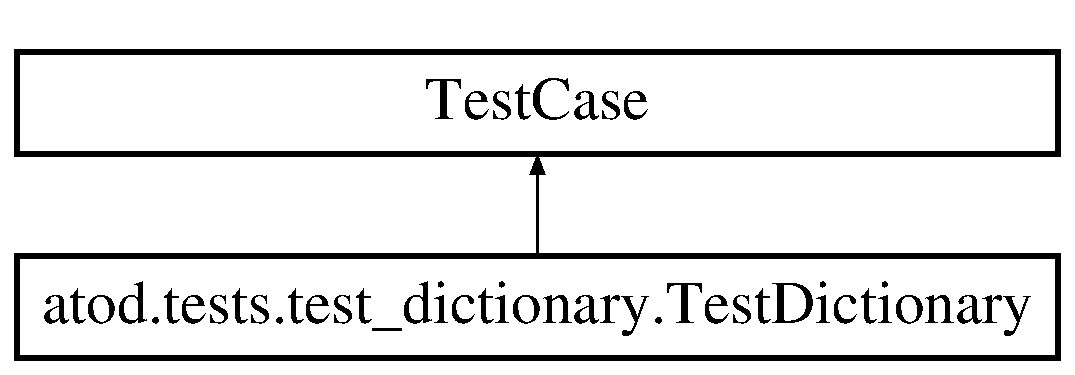
\includegraphics[height=2.000000cm]{classatod_1_1tests_1_1test__dictionary_1_1_test_dictionary}
\end{center}
\end{figure}
\subsection*{Public Member Functions}
\begin{DoxyCompactItemize}
\item 
def {\bfseries set\+Up} (self)\hypertarget{classatod_1_1tests_1_1test__dictionary_1_1_test_dictionary_ad994b8b1b6fe058db1e7f3c928d67064}{}\label{classatod_1_1tests_1_1test__dictionary_1_1_test_dictionary_ad994b8b1b6fe058db1e7f3c928d67064}

\item 
def {\bfseries test\+\_\+make\+\_\+flat\+\_\+dict} (self)\hypertarget{classatod_1_1tests_1_1test__dictionary_1_1_test_dictionary_a6d9a01d5ceca2393776cd8982a02f1ee}{}\label{classatod_1_1tests_1_1test__dictionary_1_1_test_dictionary_a6d9a01d5ceca2393776cd8982a02f1ee}

\item 
def {\bfseries test\+\_\+collect\+\_\+kv} (self)\hypertarget{classatod_1_1tests_1_1test__dictionary_1_1_test_dictionary_afdc3326ef637c4df123feb872ab3665f}{}\label{classatod_1_1tests_1_1test__dictionary_1_1_test_dictionary_afdc3326ef637c4df123feb872ab3665f}

\item 
def {\bfseries test\+\_\+all\+\_\+keys} (self)\hypertarget{classatod_1_1tests_1_1test__dictionary_1_1_test_dictionary_a9c16795d90aff317a1e63f0c4e325724}{}\label{classatod_1_1tests_1_1test__dictionary_1_1_test_dictionary_a9c16795d90aff317a1e63f0c4e325724}

\item 
def {\bfseries test\+\_\+extract\+\_\+effects} (self)\hypertarget{classatod_1_1tests_1_1test__dictionary_1_1_test_dictionary_ade63b992d7b7b4414a9603a6935fd6cf}{}\label{classatod_1_1tests_1_1test__dictionary_1_1_test_dictionary_ade63b992d7b7b4414a9603a6935fd6cf}

\item 
def {\bfseries test\+\_\+find\+\_\+all\+\_\+values} (self)\hypertarget{classatod_1_1tests_1_1test__dictionary_1_1_test_dictionary_a3d91fa1f2b3e5415ede286dbc0ce15db}{}\label{classatod_1_1tests_1_1test__dictionary_1_1_test_dictionary_a3d91fa1f2b3e5415ede286dbc0ce15db}

\item 
def {\bfseries test\+\_\+get\+\_\+types} (self)\hypertarget{classatod_1_1tests_1_1test__dictionary_1_1_test_dictionary_a7f5974ea69b973c56dcd8fe10e55db63}{}\label{classatod_1_1tests_1_1test__dictionary_1_1_test_dictionary_a7f5974ea69b973c56dcd8fe10e55db63}

\end{DoxyCompactItemize}
\subsection*{Public Attributes}
\begin{DoxyCompactItemize}
\item 
{\bfseries data\+\_\+folder}\hypertarget{classatod_1_1tests_1_1test__dictionary_1_1_test_dictionary_a6298cd582fba81f5c367ca216a71221b}{}\label{classatod_1_1tests_1_1test__dictionary_1_1_test_dictionary_a6298cd582fba81f5c367ca216a71221b}

\end{DoxyCompactItemize}


\subsection{Detailed Description}
\begin{DoxyVerb}Tests for functions from dictionary module. \end{DoxyVerb}
 

The documentation for this class was generated from the following file\+:\begin{DoxyCompactItemize}
\item 
atod/tests/test\+\_\+dictionary.\+py\end{DoxyCompactItemize}

\hypertarget{classatod_1_1tests_1_1test__hero_1_1_test_hero}{}\section{atod.\+tests.\+test\+\_\+hero.\+Test\+Hero Class Reference}
\label{classatod_1_1tests_1_1test__hero_1_1_test_hero}\index{atod.\+tests.\+test\+\_\+hero.\+Test\+Hero@{atod.\+tests.\+test\+\_\+hero.\+Test\+Hero}}
Inheritance diagram for atod.\+tests.\+test\+\_\+hero.\+Test\+Hero\+:\begin{figure}[H]
\begin{center}
\leavevmode
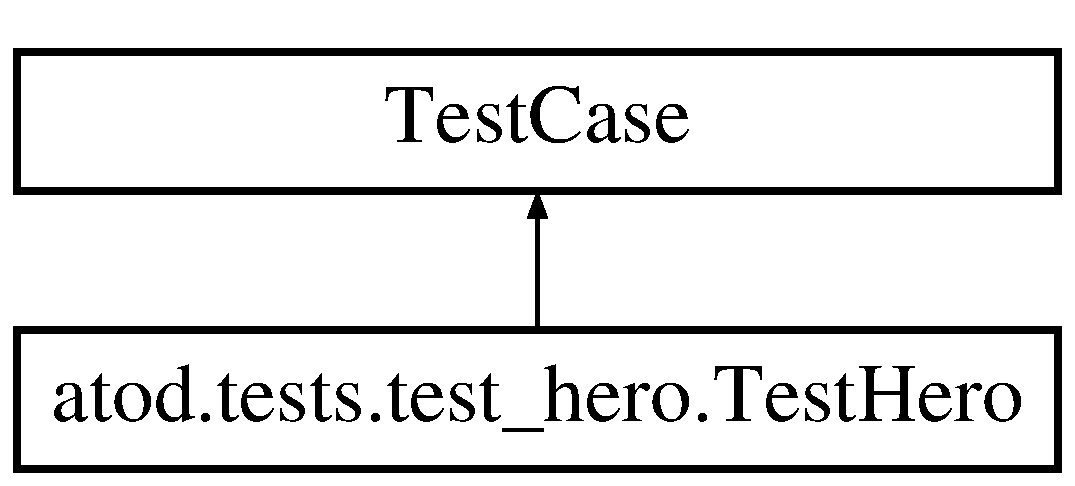
\includegraphics[height=2.000000cm]{classatod_1_1tests_1_1test__hero_1_1_test_hero}
\end{center}
\end{figure}
\subsection*{Public Member Functions}
\begin{DoxyCompactItemize}
\item 
def {\bfseries set\+Up} (self)\hypertarget{classatod_1_1tests_1_1test__hero_1_1_test_hero_a72d0d7fd2dff06de5d67ed08506d667f}{}\label{classatod_1_1tests_1_1test__hero_1_1_test_hero_a72d0d7fd2dff06de5d67ed08506d667f}

\item 
def {\bfseries test\+\_\+id} (self)\hypertarget{classatod_1_1tests_1_1test__hero_1_1_test_hero_a59ba3a7ede7a34356464678c92953664}{}\label{classatod_1_1tests_1_1test__hero_1_1_test_hero_a59ba3a7ede7a34356464678c92953664}

\item 
def {\bfseries test\+\_\+lvl} (self)\hypertarget{classatod_1_1tests_1_1test__hero_1_1_test_hero_a079911cb57f8780b93b316cfffa1538f}{}\label{classatod_1_1tests_1_1test__hero_1_1_test_hero_a079911cb57f8780b93b316cfffa1538f}

\item 
def {\bfseries test\+\_\+in\+\_\+game\+\_\+name} (self)\hypertarget{classatod_1_1tests_1_1test__hero_1_1_test_hero_a194afe7a65784ddc0c71bc50f7a0c466}{}\label{classatod_1_1tests_1_1test__hero_1_1_test_hero_a194afe7a65784ddc0c71bc50f7a0c466}

\item 
def {\bfseries test\+\_\+abilities\+\_\+adding} (self)\hypertarget{classatod_1_1tests_1_1test__hero_1_1_test_hero_a55685bf95449ca9c88393700039ab072}{}\label{classatod_1_1tests_1_1test__hero_1_1_test_hero_a55685bf95449ca9c88393700039ab072}

\end{DoxyCompactItemize}
\subsection*{Public Attributes}
\begin{DoxyCompactItemize}
\item 
{\bfseries sf\+\_\+1}\hypertarget{classatod_1_1tests_1_1test__hero_1_1_test_hero_a13aef92222c9de04db869b3ae3a6f37b}{}\label{classatod_1_1tests_1_1test__hero_1_1_test_hero_a13aef92222c9de04db869b3ae3a6f37b}

\item 
{\bfseries sf\+\_\+10}\hypertarget{classatod_1_1tests_1_1test__hero_1_1_test_hero_aebd81b2d29d3c978e0acee2c8e794ab5}{}\label{classatod_1_1tests_1_1test__hero_1_1_test_hero_aebd81b2d29d3c978e0acee2c8e794ab5}

\end{DoxyCompactItemize}


The documentation for this class was generated from the following file\+:\begin{DoxyCompactItemize}
\item 
atod/tests/test\+\_\+hero.\+py\end{DoxyCompactItemize}

\hypertarget{classatod_1_1tests_1_1test__json2vectors_1_1_test_json2_vectors}{}\section{atod.\+tests.\+test\+\_\+json2vectors.\+Test\+Json2\+Vectors Class Reference}
\label{classatod_1_1tests_1_1test__json2vectors_1_1_test_json2_vectors}\index{atod.\+tests.\+test\+\_\+json2vectors.\+Test\+Json2\+Vectors@{atod.\+tests.\+test\+\_\+json2vectors.\+Test\+Json2\+Vectors}}
Inheritance diagram for atod.\+tests.\+test\+\_\+json2vectors.\+Test\+Json2\+Vectors\+:\begin{figure}[H]
\begin{center}
\leavevmode
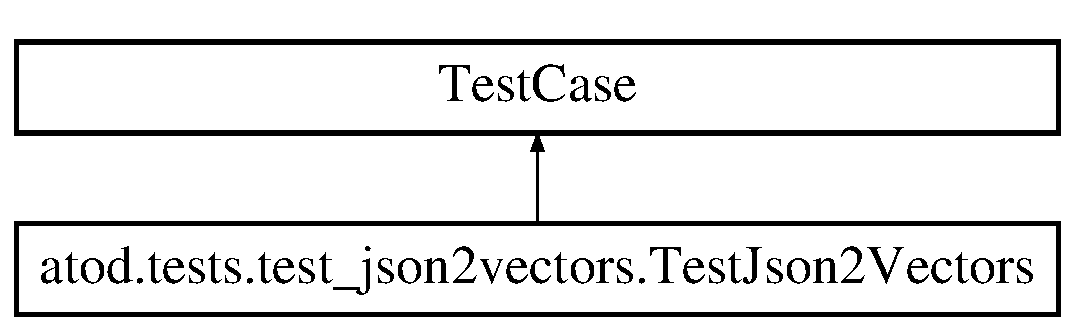
\includegraphics[height=2.000000cm]{classatod_1_1tests_1_1test__json2vectors_1_1_test_json2_vectors}
\end{center}
\end{figure}
\subsection*{Public Member Functions}
\begin{DoxyCompactItemize}
\item 
def {\bfseries test\+\_\+numeric\+\_\+part\+\_\+creation} (self)\hypertarget{classatod_1_1tests_1_1test__json2vectors_1_1_test_json2_vectors_a8f7a2f5b36f6bce066aeae763b093dc6}{}\label{classatod_1_1tests_1_1test__json2vectors_1_1_test_json2_vectors_a8f7a2f5b36f6bce066aeae763b093dc6}

\end{DoxyCompactItemize}


The documentation for this class was generated from the following file\+:\begin{DoxyCompactItemize}
\item 
atod/tests/test\+\_\+json2vectors.\+py\end{DoxyCompactItemize}

\hypertarget{classatod_1_1tests_1_1test__to__json_1_1_test_parser}{}\section{atod.\+tests.\+test\+\_\+to\+\_\+json.\+Test\+Parser Class Reference}
\label{classatod_1_1tests_1_1test__to__json_1_1_test_parser}\index{atod.\+tests.\+test\+\_\+to\+\_\+json.\+Test\+Parser@{atod.\+tests.\+test\+\_\+to\+\_\+json.\+Test\+Parser}}
Inheritance diagram for atod.\+tests.\+test\+\_\+to\+\_\+json.\+Test\+Parser\+:\begin{figure}[H]
\begin{center}
\leavevmode
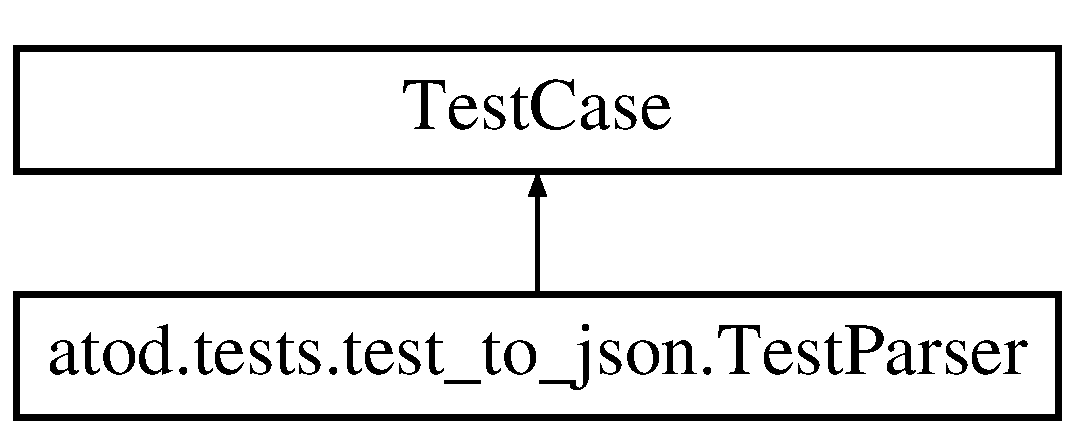
\includegraphics[height=2.000000cm]{classatod_1_1tests_1_1test__to__json_1_1_test_parser}
\end{center}
\end{figure}
\subsection*{Public Member Functions}
\begin{DoxyCompactItemize}
\item 
def \hyperlink{classatod_1_1tests_1_1test__to__json_1_1_test_parser_a3e0669b48f2fa92cf36ea7cfc283e552}{test\+\_\+comments} (self)
\item 
def \hyperlink{classatod_1_1tests_1_1test__to__json_1_1_test_parser_ae2fb42ee0ee03b5a77b0f4866120cadb}{test\+\_\+delimeters} (self)
\item 
def \hyperlink{classatod_1_1tests_1_1test__to__json_1_1_test_parser_a05a70c28fa37bb525f3f3632fe319a66}{test\+\_\+indents} (self)
\item 
def \hyperlink{classatod_1_1tests_1_1test__to__json_1_1_test_parser_aaba2235be015df76c927d18c3ce65c66}{test\+\_\+float\+\_\+fields} (self)
\item 
def \hyperlink{classatod_1_1tests_1_1test__to__json_1_1_test_parser_a38f5e65973a9b0d127b31e61fab9b6ba}{test\+\_\+empty\+\_\+value} (self)
\item 
def \hyperlink{classatod_1_1tests_1_1test__to__json_1_1_test_parser_a9e4bd96b1e5a29b91b154c4a6a2eb2fc}{test\+\_\+empty\+\_\+dict} (self)
\item 
def \hyperlink{classatod_1_1tests_1_1test__to__json_1_1_test_parser_accbb34848f3e273e3f67dffe0af6f736}{test\+\_\+symbols\+\_\+in\+\_\+values} (self)
\item 
def \hyperlink{classatod_1_1tests_1_1test__to__json_1_1_test_parser_a7cb67a3ebadc141b1fc490795ba49dee}{test\+\_\+numbers\+\_\+parsing} (self)
\end{DoxyCompactItemize}


\subsection{Detailed Description}
\begin{DoxyVerb}Test case for game files parser.

    In examples/ there are small files with all hard cases I've ran into,
    expected_*.json represents result what is expected from parser.
\end{DoxyVerb}
 

\subsection{Member Function Documentation}
\index{atod\+::tests\+::test\+\_\+to\+\_\+json\+::\+Test\+Parser@{atod\+::tests\+::test\+\_\+to\+\_\+json\+::\+Test\+Parser}!test\+\_\+comments@{test\+\_\+comments}}
\index{test\+\_\+comments@{test\+\_\+comments}!atod\+::tests\+::test\+\_\+to\+\_\+json\+::\+Test\+Parser@{atod\+::tests\+::test\+\_\+to\+\_\+json\+::\+Test\+Parser}}
\subsubsection[{\texorpdfstring{test\+\_\+comments(self)}{test\_comments(self)}}]{\setlength{\rightskip}{0pt plus 5cm}def atod.\+tests.\+test\+\_\+to\+\_\+json.\+Test\+Parser.\+test\+\_\+comments (
\begin{DoxyParamCaption}
\item[{}]{self}
\end{DoxyParamCaption}
)}\hypertarget{classatod_1_1tests_1_1test__to__json_1_1_test_parser_a3e0669b48f2fa92cf36ea7cfc283e552}{}\label{classatod_1_1tests_1_1test__to__json_1_1_test_parser_a3e0669b48f2fa92cf36ea7cfc283e552}
\begin{DoxyVerb}Tests every case of placing comments in file. \end{DoxyVerb}
 \index{atod\+::tests\+::test\+\_\+to\+\_\+json\+::\+Test\+Parser@{atod\+::tests\+::test\+\_\+to\+\_\+json\+::\+Test\+Parser}!test\+\_\+delimeters@{test\+\_\+delimeters}}
\index{test\+\_\+delimeters@{test\+\_\+delimeters}!atod\+::tests\+::test\+\_\+to\+\_\+json\+::\+Test\+Parser@{atod\+::tests\+::test\+\_\+to\+\_\+json\+::\+Test\+Parser}}
\subsubsection[{\texorpdfstring{test\+\_\+delimeters(self)}{test\_delimeters(self)}}]{\setlength{\rightskip}{0pt plus 5cm}def atod.\+tests.\+test\+\_\+to\+\_\+json.\+Test\+Parser.\+test\+\_\+delimeters (
\begin{DoxyParamCaption}
\item[{}]{self}
\end{DoxyParamCaption}
)}\hypertarget{classatod_1_1tests_1_1test__to__json_1_1_test_parser_ae2fb42ee0ee03b5a77b0f4866120cadb}{}\label{classatod_1_1tests_1_1test__to__json_1_1_test_parser_ae2fb42ee0ee03b5a77b0f4866120cadb}
\begin{DoxyVerb}Tests ways to separate strings, keys, values. \end{DoxyVerb}
 \index{atod\+::tests\+::test\+\_\+to\+\_\+json\+::\+Test\+Parser@{atod\+::tests\+::test\+\_\+to\+\_\+json\+::\+Test\+Parser}!test\+\_\+empty\+\_\+dict@{test\+\_\+empty\+\_\+dict}}
\index{test\+\_\+empty\+\_\+dict@{test\+\_\+empty\+\_\+dict}!atod\+::tests\+::test\+\_\+to\+\_\+json\+::\+Test\+Parser@{atod\+::tests\+::test\+\_\+to\+\_\+json\+::\+Test\+Parser}}
\subsubsection[{\texorpdfstring{test\+\_\+empty\+\_\+dict(self)}{test\_empty\_dict(self)}}]{\setlength{\rightskip}{0pt plus 5cm}def atod.\+tests.\+test\+\_\+to\+\_\+json.\+Test\+Parser.\+test\+\_\+empty\+\_\+dict (
\begin{DoxyParamCaption}
\item[{}]{self}
\end{DoxyParamCaption}
)}\hypertarget{classatod_1_1tests_1_1test__to__json_1_1_test_parser_a9e4bd96b1e5a29b91b154c4a6a2eb2fc}{}\label{classatod_1_1tests_1_1test__to__json_1_1_test_parser_a9e4bd96b1e5a29b91b154c4a6a2eb2fc}
\begin{DoxyVerb}Example with empty dictionary in the input file. \end{DoxyVerb}
 \index{atod\+::tests\+::test\+\_\+to\+\_\+json\+::\+Test\+Parser@{atod\+::tests\+::test\+\_\+to\+\_\+json\+::\+Test\+Parser}!test\+\_\+empty\+\_\+value@{test\+\_\+empty\+\_\+value}}
\index{test\+\_\+empty\+\_\+value@{test\+\_\+empty\+\_\+value}!atod\+::tests\+::test\+\_\+to\+\_\+json\+::\+Test\+Parser@{atod\+::tests\+::test\+\_\+to\+\_\+json\+::\+Test\+Parser}}
\subsubsection[{\texorpdfstring{test\+\_\+empty\+\_\+value(self)}{test\_empty\_value(self)}}]{\setlength{\rightskip}{0pt plus 5cm}def atod.\+tests.\+test\+\_\+to\+\_\+json.\+Test\+Parser.\+test\+\_\+empty\+\_\+value (
\begin{DoxyParamCaption}
\item[{}]{self}
\end{DoxyParamCaption}
)}\hypertarget{classatod_1_1tests_1_1test__to__json_1_1_test_parser_a38f5e65973a9b0d127b31e61fab9b6ba}{}\label{classatod_1_1tests_1_1test__to__json_1_1_test_parser_a38f5e65973a9b0d127b31e61fab9b6ba}
\begin{DoxyVerb}Example with empty value in the input file. \end{DoxyVerb}
 \index{atod\+::tests\+::test\+\_\+to\+\_\+json\+::\+Test\+Parser@{atod\+::tests\+::test\+\_\+to\+\_\+json\+::\+Test\+Parser}!test\+\_\+float\+\_\+fields@{test\+\_\+float\+\_\+fields}}
\index{test\+\_\+float\+\_\+fields@{test\+\_\+float\+\_\+fields}!atod\+::tests\+::test\+\_\+to\+\_\+json\+::\+Test\+Parser@{atod\+::tests\+::test\+\_\+to\+\_\+json\+::\+Test\+Parser}}
\subsubsection[{\texorpdfstring{test\+\_\+float\+\_\+fields(self)}{test\_float\_fields(self)}}]{\setlength{\rightskip}{0pt plus 5cm}def atod.\+tests.\+test\+\_\+to\+\_\+json.\+Test\+Parser.\+test\+\_\+float\+\_\+fields (
\begin{DoxyParamCaption}
\item[{}]{self}
\end{DoxyParamCaption}
)}\hypertarget{classatod_1_1tests_1_1test__to__json_1_1_test_parser_aaba2235be015df76c927d18c3ce65c66}{}\label{classatod_1_1tests_1_1test__to__json_1_1_test_parser_aaba2235be015df76c927d18c3ce65c66}
\begin{DoxyVerb}Example with float fields. \end{DoxyVerb}
 \index{atod\+::tests\+::test\+\_\+to\+\_\+json\+::\+Test\+Parser@{atod\+::tests\+::test\+\_\+to\+\_\+json\+::\+Test\+Parser}!test\+\_\+indents@{test\+\_\+indents}}
\index{test\+\_\+indents@{test\+\_\+indents}!atod\+::tests\+::test\+\_\+to\+\_\+json\+::\+Test\+Parser@{atod\+::tests\+::test\+\_\+to\+\_\+json\+::\+Test\+Parser}}
\subsubsection[{\texorpdfstring{test\+\_\+indents(self)}{test\_indents(self)}}]{\setlength{\rightskip}{0pt plus 5cm}def atod.\+tests.\+test\+\_\+to\+\_\+json.\+Test\+Parser.\+test\+\_\+indents (
\begin{DoxyParamCaption}
\item[{}]{self}
\end{DoxyParamCaption}
)}\hypertarget{classatod_1_1tests_1_1test__to__json_1_1_test_parser_a05a70c28fa37bb525f3f3632fe319a66}{}\label{classatod_1_1tests_1_1test__to__json_1_1_test_parser_a05a70c28fa37bb525f3f3632fe319a66}
\begin{DoxyVerb}Tests ways to separate strings, keys, values. \end{DoxyVerb}
 \index{atod\+::tests\+::test\+\_\+to\+\_\+json\+::\+Test\+Parser@{atod\+::tests\+::test\+\_\+to\+\_\+json\+::\+Test\+Parser}!test\+\_\+numbers\+\_\+parsing@{test\+\_\+numbers\+\_\+parsing}}
\index{test\+\_\+numbers\+\_\+parsing@{test\+\_\+numbers\+\_\+parsing}!atod\+::tests\+::test\+\_\+to\+\_\+json\+::\+Test\+Parser@{atod\+::tests\+::test\+\_\+to\+\_\+json\+::\+Test\+Parser}}
\subsubsection[{\texorpdfstring{test\+\_\+numbers\+\_\+parsing(self)}{test\_numbers\_parsing(self)}}]{\setlength{\rightskip}{0pt plus 5cm}def atod.\+tests.\+test\+\_\+to\+\_\+json.\+Test\+Parser.\+test\+\_\+numbers\+\_\+parsing (
\begin{DoxyParamCaption}
\item[{}]{self}
\end{DoxyParamCaption}
)}\hypertarget{classatod_1_1tests_1_1test__to__json_1_1_test_parser_a7cb67a3ebadc141b1fc490795ba49dee}{}\label{classatod_1_1tests_1_1test__to__json_1_1_test_parser_a7cb67a3ebadc141b1fc490795ba49dee}
\begin{DoxyVerb}Tests how numbers inside of "" can be converted to their values. \end{DoxyVerb}
 \index{atod\+::tests\+::test\+\_\+to\+\_\+json\+::\+Test\+Parser@{atod\+::tests\+::test\+\_\+to\+\_\+json\+::\+Test\+Parser}!test\+\_\+symbols\+\_\+in\+\_\+values@{test\+\_\+symbols\+\_\+in\+\_\+values}}
\index{test\+\_\+symbols\+\_\+in\+\_\+values@{test\+\_\+symbols\+\_\+in\+\_\+values}!atod\+::tests\+::test\+\_\+to\+\_\+json\+::\+Test\+Parser@{atod\+::tests\+::test\+\_\+to\+\_\+json\+::\+Test\+Parser}}
\subsubsection[{\texorpdfstring{test\+\_\+symbols\+\_\+in\+\_\+values(self)}{test\_symbols\_in\_values(self)}}]{\setlength{\rightskip}{0pt plus 5cm}def atod.\+tests.\+test\+\_\+to\+\_\+json.\+Test\+Parser.\+test\+\_\+symbols\+\_\+in\+\_\+values (
\begin{DoxyParamCaption}
\item[{}]{self}
\end{DoxyParamCaption}
)}\hypertarget{classatod_1_1tests_1_1test__to__json_1_1_test_parser_accbb34848f3e273e3f67dffe0af6f736}{}\label{classatod_1_1tests_1_1test__to__json_1_1_test_parser_accbb34848f3e273e3f67dffe0af6f736}
\begin{DoxyVerb}Test different unusual symbols in values. \end{DoxyVerb}
 

The documentation for this class was generated from the following file\+:\begin{DoxyCompactItemize}
\item 
atod/tests/test\+\_\+to\+\_\+json.\+py\end{DoxyCompactItemize}

\hypertarget{classatod_1_1tests_1_1test__settings_1_1_test_settings}{}\section{atod.\+tests.\+test\+\_\+settings.\+Test\+Settings Class Reference}
\label{classatod_1_1tests_1_1test__settings_1_1_test_settings}\index{atod.\+tests.\+test\+\_\+settings.\+Test\+Settings@{atod.\+tests.\+test\+\_\+settings.\+Test\+Settings}}
Inheritance diagram for atod.\+tests.\+test\+\_\+settings.\+Test\+Settings\+:\begin{figure}[H]
\begin{center}
\leavevmode
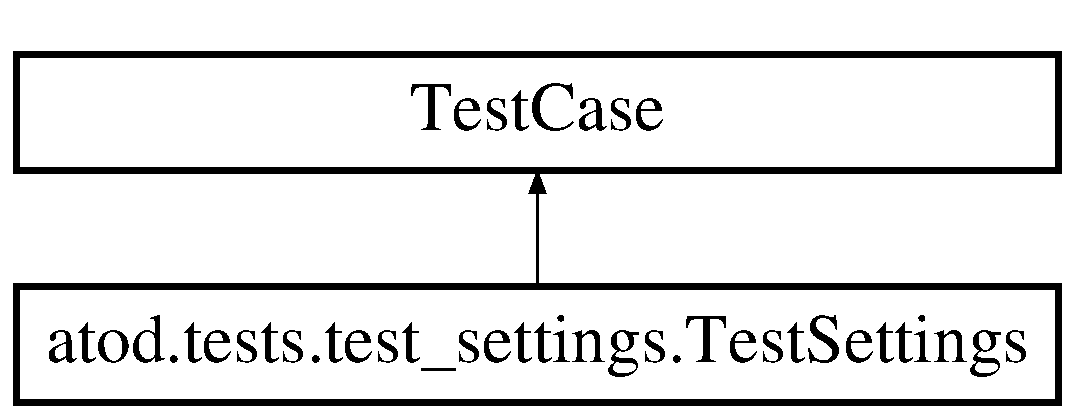
\includegraphics[height=2.000000cm]{classatod_1_1tests_1_1test__settings_1_1_test_settings}
\end{center}
\end{figure}
\subsection*{Public Member Functions}
\begin{DoxyCompactItemize}
\item 
def \hyperlink{classatod_1_1tests_1_1test__settings_1_1_test_settings_a8faa49511d50365876e9576c4848c5cd}{test\+\_\+existance} (self)
\end{DoxyCompactItemize}


\subsection{Detailed Description}
\begin{DoxyVerb}Class to test atod.settings.py files

    Checks existance of all the needed files.
\end{DoxyVerb}
 

\subsection{Member Function Documentation}
\index{atod\+::tests\+::test\+\_\+settings\+::\+Test\+Settings@{atod\+::tests\+::test\+\_\+settings\+::\+Test\+Settings}!test\+\_\+existance@{test\+\_\+existance}}
\index{test\+\_\+existance@{test\+\_\+existance}!atod\+::tests\+::test\+\_\+settings\+::\+Test\+Settings@{atod\+::tests\+::test\+\_\+settings\+::\+Test\+Settings}}
\subsubsection[{\texorpdfstring{test\+\_\+existance(self)}{test\_existance(self)}}]{\setlength{\rightskip}{0pt plus 5cm}def atod.\+tests.\+test\+\_\+settings.\+Test\+Settings.\+test\+\_\+existance (
\begin{DoxyParamCaption}
\item[{}]{self}
\end{DoxyParamCaption}
)}\hypertarget{classatod_1_1tests_1_1test__settings_1_1_test_settings_a8faa49511d50365876e9576c4848c5cd}{}\label{classatod_1_1tests_1_1test__settings_1_1_test_settings_a8faa49511d50365876e9576c4848c5cd}
\begin{DoxyVerb}Tests existance of files mentioned in settings.

    Files names variables have caps-locked names.
\end{DoxyVerb}
 

The documentation for this class was generated from the following file\+:\begin{DoxyCompactItemize}
\item 
atod/tests/test\+\_\+settings.\+py\end{DoxyCompactItemize}

\hypertarget{classtest__abilities_1_1_test_tools_abilities}{}\section{test\+\_\+abilities.\+Test\+Tools\+Abilities Class Reference}
\label{classtest__abilities_1_1_test_tools_abilities}\index{test\+\_\+abilities.\+Test\+Tools\+Abilities@{test\+\_\+abilities.\+Test\+Tools\+Abilities}}
Inheritance diagram for test\+\_\+abilities.\+Test\+Tools\+Abilities\+:\begin{figure}[H]
\begin{center}
\leavevmode
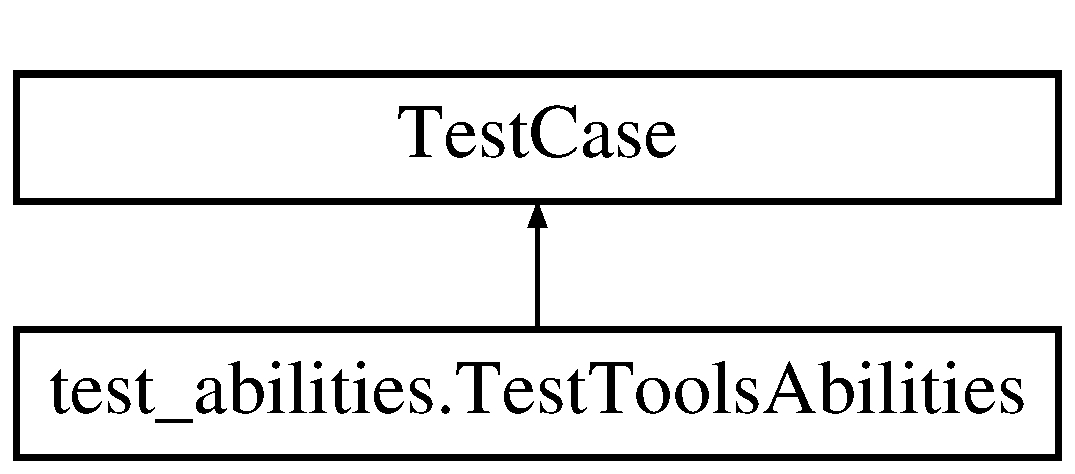
\includegraphics[height=2.000000cm]{classtest__abilities_1_1_test_tools_abilities}
\end{center}
\end{figure}
\subsection*{Public Member Functions}
\begin{DoxyCompactItemize}
\item 
def {\bfseries set\+Up} (self)\hypertarget{classtest__abilities_1_1_test_tools_abilities_a5241ad737650b495e3a3753a900db47f}{}\label{classtest__abilities_1_1_test_tools_abilities_a5241ad737650b495e3a3753a900db47f}

\item 
def {\bfseries test\+\_\+numeric} (self)\hypertarget{classtest__abilities_1_1_test_tools_abilities_a4f2a227cfb70263ccaf5015942e02a30}{}\label{classtest__abilities_1_1_test_tools_abilities_a4f2a227cfb70263ccaf5015942e02a30}

\item 
def {\bfseries test\+\_\+categorical} (self)\hypertarget{classtest__abilities_1_1_test_tools_abilities_a04c4ff9cfd0b78060f582ea122a6ade3}{}\label{classtest__abilities_1_1_test_tools_abilities_a04c4ff9cfd0b78060f582ea122a6ade3}

\end{DoxyCompactItemize}
\subsection*{Public Attributes}
\begin{DoxyCompactItemize}
\item 
{\bfseries data\+\_\+folder}\hypertarget{classtest__abilities_1_1_test_tools_abilities_a4c152c7433c0021e28ab194a6912b2cc}{}\label{classtest__abilities_1_1_test_tools_abilities_a4c152c7433c0021e28ab194a6912b2cc}

\end{DoxyCompactItemize}


The documentation for this class was generated from the following file\+:\begin{DoxyCompactItemize}
\item 
deprecated/test\+\_\+abilities.\+py\end{DoxyCompactItemize}

\hypertarget{classatod_1_1tests_1_1test__to__rows_1_1_test_utils_d_b}{}\section{atod.\+tests.\+test\+\_\+to\+\_\+rows.\+Test\+Utils\+DB Class Reference}
\label{classatod_1_1tests_1_1test__to__rows_1_1_test_utils_d_b}\index{atod.\+tests.\+test\+\_\+to\+\_\+rows.\+Test\+Utils\+DB@{atod.\+tests.\+test\+\_\+to\+\_\+rows.\+Test\+Utils\+DB}}
Inheritance diagram for atod.\+tests.\+test\+\_\+to\+\_\+rows.\+Test\+Utils\+DB\+:\begin{figure}[H]
\begin{center}
\leavevmode
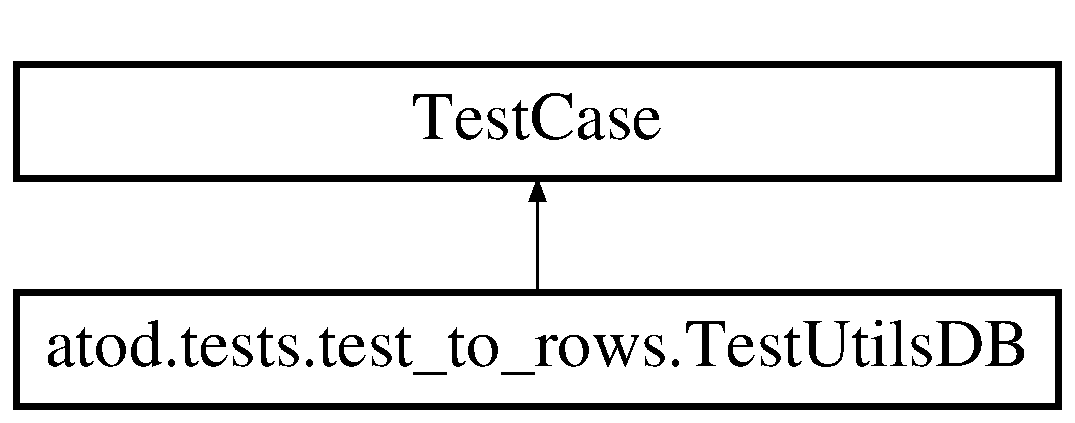
\includegraphics[height=2.000000cm]{classatod_1_1tests_1_1test__to__rows_1_1_test_utils_d_b}
\end{center}
\end{figure}
\subsection*{Public Member Functions}
\begin{DoxyCompactItemize}
\item 
def {\bfseries set\+Up} (self)\hypertarget{classatod_1_1tests_1_1test__to__rows_1_1_test_utils_d_b_afb201e7c93ce0e6f583950fc035d9df9}{}\label{classatod_1_1tests_1_1test__to__rows_1_1_test_utils_d_b_afb201e7c93ce0e6f583950fc035d9df9}

\item 
def {\bfseries test\+\_\+abilities\+\_\+to\+\_\+rows} (self)\hypertarget{classatod_1_1tests_1_1test__to__rows_1_1_test_utils_d_b_a7c8aa3dc51d185b1d9ecb064d8678aae}{}\label{classatod_1_1tests_1_1test__to__rows_1_1_test_utils_d_b_a7c8aa3dc51d185b1d9ecb064d8678aae}

\end{DoxyCompactItemize}
\subsection*{Public Attributes}
\begin{DoxyCompactItemize}
\item 
{\bfseries data\+\_\+folder}\hypertarget{classatod_1_1tests_1_1test__to__rows_1_1_test_utils_d_b_ae0cf5fd9b810c6072070db59f24b3aac}{}\label{classatod_1_1tests_1_1test__to__rows_1_1_test_utils_d_b_ae0cf5fd9b810c6072070db59f24b3aac}

\end{DoxyCompactItemize}


The documentation for this class was generated from the following file\+:\begin{DoxyCompactItemize}
\item 
atod/tests/test\+\_\+to\+\_\+rows.\+py\end{DoxyCompactItemize}

%--- End generated contents ---

% Index
\backmatter
\newpage
\phantomsection
\clearemptydoublepage
\addcontentsline{toc}{chapter}{Index}
\printindex

\end{document}
